\documentclass[3p,11pt,draft,natbib=false]{elsarticle}
% \usepackage[backend=biber]{biblatex}
% \addbibresource{references.bib} % Cambia 'bibliografia.bib' por el nombre de tu archivo .bib

% ========================================
% PAQUETES ESENCIALES
% ========================================
\usepackage[utf8]{inputenc}
\usepackage[T1]{fontenc}
\usepackage[spanish]{babel}

% ========================================
% MATEMÁTICAS
% ========================================
\usepackage{amsmath}
\usepackage{amssymb}
\usepackage{amsthm}
\usepackage{mathtools}

% ========================================
% GRÁFICOS Y FIGURAS
% ========================================
\usepackage{graphicx}
\usepackage{float}
\usepackage{subcaption}
\usepackage{tikz}
\usepackage{pgfplots}
\pgfplotsset{compat=1.18}

% Configuración de la ruta de figuras
\graphicspath{{../../notebooks/figures/}{../../reports/figures/}}

% Configuración de floats
% \floatsetup[figure]{capposition=top}
% \floatsetup[table]{capposition=top}

% ========================================
% TABLAS
% ========================================
\usepackage{booktabs}
\usepackage{multirow}
\usepackage{makecell}
\usepackage{array}
\usepackage{longtable}

% ========================================
% FORMATO Y ESTILO
% ========================================
\usepackage{siunitx}
\usepackage{xcolor}
\usepackage{enumitem}

% Configuración de siunitx para números
\sisetup{
    round-mode=places,
    round-precision=3,
    detect-weight=true,
    detect-inline-weight=math
}

% ========================================
% REFERENCIAS Y ENLACES
% ========================================
\usepackage{hyperref}
\usepackage{cleveref}

% Configuración de bibliografía con biblatex en formato APA
\usepackage[style=apa,
            backend=biber,
            natbib=false,
            sorting=nyt,
            maxcitenames=2,
            maxbibnames=99,
            uniquename=false,
            uniquelist=false,
            url=true,
            doi=true]{biblatex}
\DeclareLanguageMapping{spanish}{spanish-apa}
\addbibresource{references.bib}

% Configuración de hyperref
\hypersetup{
    colorlinks=true,
    linkcolor=blue,
    citecolor=blue,
    urlcolor=blue,
    pdfauthor={Manuel Alejandro Hidalgo Pérez},
    pdftitle={Indicador de Vulnerabilidad Externa Model-Implied para Brasil}
}



% ========================================
% COMANDOS PERSONALIZADOS MATEMÁTICOS
% ========================================
\newcommand{\E}{\mathbb{E}}
\newcommand{\Var}{\mathbb{V}\text{ar}}
\newcommand{\Cov}{\mathbb{C}\text{ov}}
\newcommand{\R}{\mathbb{R}}
\newcommand{\vect}[1]{\boldsymbol{#1}}

% Operadores personalizados
\DeclareMathOperator*{\argmax}{arg\,max}
\DeclareMathOperator*{\argmin}{arg\,min}

% ========================================
% FORMATO DE PÁRRAFOS
% ========================================
\setlength{\parindent}{0pt}        
\setlength{\parskip}{6pt}

% ========================================
% LÍNEAS DE NUMERACIÓN (opcional, para revisión)
% ========================================
\usepackage{lineno}
% \linenumbers  % Descomentar para activar numeración de líneas

% ========================================
% INFORMACIÓN DEL DOCUMENTO
% ========================================
\begin{document}

\begin{frontmatter}

\title{Indicador de Vulnerabilidad Externa Model-Implied para Brasil: \\ 
Una Extensión del Marco VECM con IRFs y Riesgo Dinámico}

\author[inst1]{Manuel Alejandro Hidalgo Pérez}
\ead{mhidper@upo.es}

\author[inst1]{Ernesto Talvi}
\ead{etalvi@realinstitutoelcano.org}

\address[inst1]{Real Instituto Elcano, Madrid, España}

\begin{abstract}
Este documento desarrolla un indicador de vulnerabilidad externa \emph{model-implied} para Brasil mediante un Modelo de Vectores de Corrección de Errores (VECM) que integra tres dimensiones analíticas: (i) desequilibrios de largo plazo medidos por el término de corrección de error, (ii) sensibilidades dinámicas del PIB a shocks externos mediante funciones impulso-respuesta, y (iii) riesgo externo vigente capturado por matrices de covarianzas rolling de los shocks fundamentales. 

La metodología extiende el trabajo seminal de Izquierdo, Romero y Talvi (2008) desde un enfoque retrospectivo de descomposición hacia un sistema prospectivo de alerta temprana. El indicador combina el empuje contractivo del equilibrio (\(\mu_t\)) con el riesgo agregado externo (\(\sigma_t\)) en una métrica normalizada por volatilidad, amplificada en períodos de alta incertidumbre. Esta especificación permite: (i) trazabilidad completa por variables de equilibrio y fuentes de shock, (ii) ausencia de ponderaciones arbitrarias (los pesos provienen del modelo estimado), y (iii) portabilidad metodológica entre países y períodos.

Los resultados para Brasil (2000Q1-2024Q4, 99 observaciones) validan la capacidad predictiva del indicador: correlación significativa con crecimiento futuro del PIB (-0.223 a horizonte de 2 trimestres), identificación correcta de todos los episodios históricos de crisis (2002-2003, 2008-2009, 2014-2016, 2020), y descomposiciones interpretables que atribuyen la vulnerabilidad a canales específicos (términos de intercambio, condiciones financieras globales, spreads soberanos). El marco es extensible a análisis multipaís y escenarios contrafactuales de política.
\end{abstract}

\begin{keyword}
Vulnerabilidad externa \sep VECM \sep Funciones impulso-respuesta \sep Riesgo dinámico \sep Alerta temprana \sep Indicador model-implied \sep Cointegración
% \MSC[2010] 62M10, 62P20
% \JEL C32, C53, F34, F47, O54
\end{keyword}

\end{frontmatter}

% ========================================
% CUERPO DEL DOCUMENTO
% ========================================

\section{Introducción}
\label{sec:intro}

Las economías latinoamericanas exportadoras de materias primas enfrentan una exposición estructural a la volatilidad del entorno económico global. Las fluctuaciones en los precios de commodities, los cambios en las condiciones financieras internacionales, las variaciones en la demanda de los principales socios comerciales y los movimientos en los flujos de capital pueden generar shocks externos de magnitud considerable, con profundas repercusiones sobre el crecimiento económico, la estabilidad macroeconómica y la sostenibilidad fiscal. En este contexto, el desarrollo de herramientas robustas y oportunas para el monitoreo y la predicción de episodios de vulnerabilidad externa constituye una prioridad fundamental para la formulación de políticas macroeconómicas efectivas y la gestión proactiva del riesgo sistémico.

Responsables de política económica y gestores de riesgo necesitan responder a tres preguntas esenciales cuando evalúan la vulnerabilidad externa de sus economías. La primera es qué tanta presión contractiva sugiere hoy el modelo: dado el desvío respecto al equilibrio externo y su velocidad de ajuste, cuál es el empuje previsto sobre el crecimiento a corto plazo. La segunda pregunta concierne a cuánta incertidumbre externa enfrenta ese empuje: el mismo impulso puede ser más o menos preocupante según la volatilidad y las covarianzas recientes de los shocks relevantes. Finalmente, la tercera pregunta busca identificar qué canal está detrás de cada episodio: para que la métrica sea accionable debe permitir atribuir cambios del indicador a variables del equilibrio (comercio, tasas globales) o a fuentes específicas de riesgo (términos de intercambio, condiciones financieras, spreads soberanos), evitando índices opacos con ponderaciones discrecionales.

El trabajo seminal de \citet{izquierdo2008booms} estableció un marco metodológico fundamental para el análisis econométrico de la vulnerabilidad externa en América Latina mediante la aplicación de un Modelo de Vectores de Corrección de Errores. Su enfoque permitió descomponer las fluctuaciones del PIB agregado regional en componentes atribuibles a shocks externos versus dinámicas internas, proporcionando una cuantificación rigurosa del papel de los factores externos en los ciclos económicos latinoamericanos. El modelo se centra en el análisis retrospectivo mediante funciones impulso-respuesta, permitiendo realizar ejercicios contrafactuales que evalúan cómo habría evolucionado el PIB regional bajo escenarios alternativos de condiciones externas. Esta aproximación proporciona una comprensión profunda de los mecanismos de transmisión de shocks externos y su descomposición causal.

El presente estudio se fundamenta en esta sólida base econométrica y la extiende en direcciones que responden a necesidades operacionales complementarias para el monitoreo de vulnerabilidad externa. Las diferencias metodológicas entre ambos enfoques no constituyen una divergencia conceptual, sino una evolución natural hacia objetivos analíticos distintos pero complementarios. Mientras el trabajo de \citet{izquierdo2008booms} proporciona una comprensión profunda de los mecanismos de transmisión de shocks externos y su descomposición causal, este estudio desarrolla una herramienta sintética orientada específicamente hacia la detección temprana y el monitoreo sistemático de episodios de vulnerabilidad.

La primera diferencia metodológica fundamental radica en la especificación geográfica y temporal del análisis. El modelo original analiza un índice agregado LAC7 que captura comportamientos promedio regionales en el período 1970-2004, proporcionando insights sobre dinámicas estructurales de largo plazo para América Latina como conjunto. Este trabajo, en contraste, desarrolla modelos país-específicos calibrados para economías individuales (con Brasil como caso de estudio), utilizando datos más recientes (2000-2024) que incorporan episodios críticos posteriores como la crisis financiera global de 2008-2009, la desaceleración de commodities de 2012-2015, y el shock pandémico de 2020-2021. Esta especificación permite capturar heterogeneidades estructurales específicas de cada país que se diluyen en agregados regionales, como la importancia particular de ciertos commodities en la canasta exportadora o la sensibilidad específica a condiciones financieras globales dada la profundidad relativa del mercado de capitales.

La segunda diferencia metodológica central se relaciona con el objetivo analítico y el tipo de output generado. El enfoque original se orienta hacia la comprensión causal y la descomposición explicativa mediante funciones impulso-respuesta, proporcionando información detallada sobre la velocidad y magnitud de las respuestas del PIB ante diferentes tipos de shocks externos. Este análisis es fundamental para el diseño de políticas de estabilización y la comprensión de canales de transmisión específicos. El presente trabajo, en cambio, construye un indicador sintético que combina el desequilibrio respecto al equilibrio de largo plazo (derivado del VECM) con el riesgo externo vigente (medido a través de covarianzas de shocks y respuestas impulso-respuesta). El índice final pondera el empuje contractivo sugerido por el modelo en unidades de riesgo y lo amplifica por el nivel de incertidumbre observado. Esta transformación convierte el VECM de una herramienta de análisis retrospectivo en un sistema de alerta temprana cuantitativamente validado.

La tercera innovación metodológica consiste en el diseño model-implied del indicador. A diferencia de los índices compuestos tradicionales que asignan pesos arbitrarios o heurísticos a sus componentes, nuestra aproximación extrae todas las ponderaciones directamente del modelo estimado. El desequilibrio proviene del término de corrección del error y su velocidad de ajuste estimada, mientras que el riesgo se deriva de las funciones impulso-respuesta del PIB y de la matriz de covarianzas empírica de los shocks. Esta especificación garantiza coherencia teórica con el modelo subyacente y permite una trazabilidad completa: cada observación del indicador puede descomponerse en contribuciones de variables individuales del equilibrio y de fuentes específicas de shock. Así, el indicador no es una media ponderada ad-hoc, sino una síntesis que refleja las dinámicas estructurales identificadas econométricamente.

La cuarta extensión se centra en la evaluación sistemática de capacidad predictiva mediante métricas de desempeño estadístico. Mientras el enfoque original se concentra en explicar variaciones históricas del PIB mediante validación econométrica estándar (coeficientes de determinación, significancia estadística, diagnósticos de residuos), este trabajo evalúa rigurosamente la capacidad del indicador para anticipar episodios futuros de vulnerabilidad. Se implementan análisis de correlación cruzada con múltiples horizontes temporales, curvas ROC para evaluar precisión en la clasificación de crisis, y técnicas de validación fuera de muestra mediante ventanas móviles. Esta orientación prospectiva es fundamental para establecer la credibilidad del indicador como herramienta operacional de política económica, proporcionando evidencia cuantitativa sobre su utilidad práctica para la detección temprana de episodios de riesgo.

Es importante enfatizar que estos enfoques metodológicos son fundamentalmente complementarios en la práctica del análisis macroeconómico. El marco original resulta particularmente valioso para comprender las fuentes granulares y específicas de vulnerabilidad, identificar canales de transmisión particulares, y proporcionar un contexto interpretativo rico para el análisis cualitativo de episodios históricos. El poder explicativo de las funciones impulso-respuesta permite responder preguntas como: ¿en qué medida la recesión de 2008-2009 fue atribuible a shocks en términos de intercambio versus endurecimiento de condiciones financieras globales? Por su parte, el indicador sintético desarrollado en este trabajo optimiza la capacidad de detección temprana mediante la síntesis de múltiples dimensiones de riesgo en una métrica única, temporalmente comparable y cuantitativamente validada. Su utilidad se manifiesta en la capacidad para responder preguntas prospectivas: ¿cuál es el nivel actual de vulnerabilidad externa? ¿se está aproximando a umbrales históricamente asociados con episodios de crisis?

La síntesis metodológica óptima combinaría el poder explicativo retrospectivo del modelo original con la capacidad predictiva prospectiva del indicador desarrollado en este trabajo. En un sistema de monitoreo integral, el indicador sintético podría funcionar como sistema de alerta temprana que, al superar umbrales predefinidos, activaría análisis más detallados mediante funciones impulso-respuesta para identificar las fuentes específicas de vulnerabilidad y diseñar respuestas de política apropiadas. Esta integración maximizaría tanto la profundidad analítica como la eficiencia operacional del sistema de monitoreo, combinando la riqueza interpretativa del enfoque desagregado con la objetividad y sistematicidad del enfoque sintético.

El resto del documento se estructura de la siguiente manera. La Sección \ref{sec:literatura} presenta la revisión de la literatura sobre vulnerabilidad externa, indicadores compuestos y metodologías econométricas relacionadas. La Sección \ref{sec:metodologia} presenta la metodología econométrica, describiendo los datos, las pruebas de estacionariedad y cointegración, la especificación del modelo VECM, las funciones impulso-respuesta, y la construcción de la matriz de covarianzas rolling. La Sección \ref{sec:indicador} detalla la construcción del indicador model-implied de vulnerabilidad externa, incluyendo la definición de sus componentes (desequilibrio y riesgo), el índice final con amplificador, y las descomposiciones que permiten trazabilidad completa. La Sección \ref{sec:resultados} presenta los resultados empíricos, validando el modelo mediante tests diagnósticos y evaluando la capacidad predictiva del indicador para identificar episodios históricos de crisis. Finalmente, la Sección \ref{sec:conclusiones} concluye con una síntesis de las principales contribuciones y sugerencias para investigación futura.

\section{Revisión de Literatura}
\label{sec:literatura}

La necesidad de herramientas sistemáticas para el monitoreo de vulnerabilidad externa en economías emergentes ha motivado una literatura extensa que abarca desde sistemas de alerta temprana tradicionales hasta indicadores compuestos sofisticados. Mientras investigación previa ha empleado modelos VECM extensamente para análisis de transmisión de shocks en mercados emergentes y desarrollado indicadores comprehensivos de vulnerabilidad financiera, a nuestro conocimiento ningún estudio ha integrado términos de corrección de error derivados de VECM, funciones impulso-respuesta VECM-based, y estructuras de covarianza rolling de residuos VECM en un indicador de vulnerabilidad externa model-implied unificado. Este trabajo llena esta brecha extendiendo el marco seminal de Izquierdo, Romero y Talvi (2008) desde análisis retrospectivo hacia sistema prospectivo de alerta temprana, con todas las componentes derivadas endógenamente de parámetros estimados sin ponderaciones arbitrarias.

\subsection{Vulnerabilidad Externa en América Latina: La Tradición del BID}

El trabajo fundacional de \citet{izquierdo2008booms} \textit{Booms and Busts in Latin America: The Role of External Factors} estableció el marco retrospectivo mediante VECM para analizar economías latinoamericanas durante 1990-2006, demostrando empíricamente que factores externos explican porción significativa de la varianza del crecimiento del PIB regional. Los shocks externos producen respuestas de magnitud considerable y persistentes. Este trabajo establece relevancia empírica de drivers externos pero mantiene enfoque retrospectivo: explica qué ocurrió históricamente sin construir sistema prospectivo de alerta temprana.

Esta línea se fundamenta en investigación sobre sudden stops desarrollada por Calvo, Izquierdo y Talvi. \citet{calvo2003sudden} identificaron indicadores de vulnerabilidad que diferenciaron Argentina de economías pares durante crisis rusa 1998: apreciación de tipo de cambio real causa estragos en países con pasivos altamente dolarizados, y cambio requerido en precios relativos es mayor en economías más cerradas. \citet{calvo2005sudden} compararon respuestas de Chile versus Argentina ante crisis rusa, atribuyendo diferencias a mayor apertura comercial de Chile y menores descalces monetarios en balance. La transición crítica de análisis retrospectivo a monitoreo en tiempo real ocurrió con \citet{talvi2013latin} desarrollando External Conditions Index (ECI) basado en Izquierdo, Romero y Talvi (2008), construyendo promedio ponderado de tres drivers externos: términos de intercambio, crecimiento en socios comerciales, y condiciones financieras globales medidas por spreads EMBI, transformando marco retrospectivo en herramienta de monitoreo contemporáneo, aunque ponderaciones permanecen establecidas ex-ante por investigadores, no derivadas de modelo estructural estimado.

\citet{cavallo2023external} desarrollan External Vulnerability Assessment (EVA) mediante modelos probit actualizando indicador de crisis de \citet{catao2014external} hasta 2019, con seis indicadores de riesgo. Encuentran que economía latinoamericana promedio está en mínimo histórico de vulnerabilidad externa pero permanece más vulnerable que economías avanzadas. Este representa marco prospectivo de alerta temprana genuino generando probabilidades de crisis futuras, pero emplea modelos de forma reducida (probit) en lugar de sistemas estructurales dinámicos.

\subsection{Fundamentos Econométricos: Cointegración, IRFs y Riesgo Dinámico}

Cada componente metodológico del enfoque propuesto posee raíces teóricas profundas en corrientes econométricas establecidas, pero estas corrientes no se han integrado previamente en contexto específico de indicadores de vulnerabilidad externa. Los términos de corrección de error como medidas de desequilibrio derivan de revolución de cointegración. \citet{engle1987cointegration} establecieron relación fundamental entre cointegración y modelos de corrección de error: variables cointegradas pueden representarse como modelos de corrección de error donde término de corrección de error captura desviaciones del equilibrio de largo plazo. \citet{johansen1988statistical,johansen1991estimation} desarrolló marco de máxima verosimilitud para analizar vectores de cointegración en sistemas multivariados. Sin embargo, literatura econométrica no emplea magnitudes del ECT explícitamente como componentes de indicadores de vulnerabilidad—los ECTs se interpretan principalmente como velocidades de ajuste hacia equilibrio, no como señales de fragilidad acumulada del sistema.

Las funciones impulso-respuesta para medir vulnerabilidad tienen origen en revolución VAR de \citet{sims1980macroeconomics} estableciendo IRFs como herramienta clave para análisis dinámico de propagación de shocks. \citet{pesaran1998generalized} desarrollaron Generalized Impulse Response Functions invariantes al ordenamiento de variables, particularmente útiles para modelos VECM. Aplicaciones a vulnerabilidad de mercados emergentes incluyen \citet{canova2005transmission} demostrando que aproximadamente 50\% de variación del ciclo económico en América Latina es impulsada por shocks estadounidenses, y \citet{rey2015dilemma} usando persistencia y magnitudes de IRF para medir vulnerabilidad financiera. Las IRFs se emplean extensamente para analizar transmisión de shocks, pero magnitudes y perfiles de persistencia de IRFs no se incorporan sistemáticamente como componentes de indicadores sintéticos de vulnerabilidad.

Las covarianzas rolling y time-varying para estimación de riesgo se fundamentan en literatura de heterocedasticidad condicional. \citet{engle1982autoregressive} introdujo modelos ARCH para volatilidad time-varying, fundamento de modelado de varianza condicional. \citet{bollerslev1986generalized} extendió ARCH a GARCH. \citet{engle2002dynamic} desarrolló Dynamic Conditional Correlation (DCC-GARCH) permitiendo correlaciones time-varying en contexto multivariado. Aplicaciones a riesgo sistémico incluyen \citet{adrian2016covar} desarrollando CoVaR mediante regresiones cuantílicas, incorporando covarianzas de shocks time-varying para medir spillovers de riesgo sistémico. Matrices de covarianza rolling se emplean extensamente en gestión de riesgo y análisis de contagio, pero típicamente se estiman de datos crudos o modelos GARCH independientes, no de residuos estructurales de sistemas VECM integrados con análisis de equilibrio.

\subsection{Sistemas de Alerta Temprana y Metodologías Alternativas}

El FMI desarrolló sistemas comprehensivos desde finales de 1990s. \citet{kaminsky1998leading} publicaron trabajo seminal sobre ``signals approach'': monitorean variables individuales que se comportan inusualmente en períodos precediendo crisis, cada indicador genera señal cuando cruza umbral óptimo calibrado. \citet{kaminsky1999twin} establecieron concepto de ``twin crises'', demostrando que crisis bancarias y cambiarias están frecuentemente vinculadas. \citet{goldstein2000assessing} proveen batería comprehensiva de tests empíricos sobre performance de indicadores alternativos de alerta temprana. \citet{berg2004assessing} evaluaron sistemáticamente múltiples modelos EWS encontrando performance mixta fuera de muestra. \citet{bussiere2006towards} propusieron modelo multinomial logit mejorado distinguiendo periodos tranquilos, crisis y post-crisis.

El trabajo más cercano conceptualmente es \citet{ayvazyan2025financial} del FMI desarrollando Systemic Vulnerabilities Index usando análisis de componentes principales para ranking de variables, simulaciones Monte Carlo para selección óptima de pesos, matriz de varianza-covarianza time-varying vía exponentially weighted moving average, y agregación basada en teoría de portafolio, aplicado a Estados Unidos e Islandia. Crucialmente, este enfoque no es VECM-based, no utiliza términos de corrección de error ni funciones impulso-respuesta como inputs. \citet{hollo2012ciss} del BCE desarrollaron Composite Indicator of Systemic Stress (CISS) para área euro usando teoría de portafolio con correlaciones time-varying, agregando 15 medidas de estrés financiero en 5 segmentos de mercado, pero mide realización de estrés actual no acumulación prospectiva de vulnerabilidad, y tampoco deriva de framework VECM.

Methodologías alternativas revelan trade-off fundamental entre interpretabilidad económica versus precisión predictiva. Análisis de Componentes Principales provee ponderaciones objetivas basadas en varianza explicada pero componentes carecen de interpretación intuitiva. Machine Learning para predicción de crisis ha demostrado performance superior fuera de muestra (\citet{buckmann2023credit,reimann2024machine}) capturando no-linealidades e interacciones automáticamente, pero naturaleza ``black box'' dificulta interpretación estructural. Modelos Markov-switching capturan cambios de régimen y dinámicas no-lineales pero path dependence dificulta predicción de regime switches. Modelos probit/logit son estándar en literatura EWS proveyendo coeficientes interpretables pero suponen relación lineal en índice con inestabilidad paramétrica potencial.

\subsection{Contribución del Presente Trabajo}

La revisión exhaustiva identifica cinco brechas críticas que el enfoque VECM-based propuesto llenaría. Primera, ausencia de indicadores completamente model-implied basados en cointegración estructural: literatura existente emplea indicadores compuestos con ponderaciones ad-hoc (ECI de Talvi-Munyo, EVA de Cavallo et al., CISS del BCE) o modelos de forma reducida sin relaciones estructurales de largo plazo (probit/logit). El enfoque propuesto es completamente model-implied: términos de corrección de error midiendo desequilibrio, IRFs midiendo sensibilidad dinámica, y covarianzas rolling midiendo riesgo—todas derivan exclusivamente de parámetros estimados del mismo sistema econométrico estructural.

Segunda, no explotación de términos de corrección de error como medidas directas de vulnerabilidad acumulada: aunque literatura econométrica interpreta ECTs como velocidades de ajuste hacia equilibrio, magnitudes de ECTs no se emplean explícitamente como componentes de indicadores de vulnerabilidad en literatura de early warning systems. La innovación conceptual es reconocer que distancia del sistema respecto a trayectoria de equilibrio sostenible—capturada por magnitud del ECT—constituye señal directa de fragilidad acumulada.

Tercera, no incorporación sistemática de perfiles de IRF en construcción de índices compuestos: IRFs se emplean extensamente para analizar propagación de shocks pero magnitudes, persistencia y patrones temporales no se incorporan sistemáticamente como componentes de indicadores sintéticos. La innovación es usar perfiles completos de IRF para cuantificar dimensión de sensibilidad. Cuarta, desconexión entre análisis retrospectivo de drivers históricos y sistemas prospectivos: ningún trabajo unifica explicación retrospectiva estructural Y forecasting prospectivo dinámico en marco unificado derivado de relaciones de equilibrio económico. VECM naturalmente une ambas dimensiones temporales.

Quinta, tratamiento fragmentado de tres dimensiones conceptualmente complementarias: literatura trata separadamente equilibrio y desequilibrios, sensibilidad y transmisión de shocks, y riesgo e interdependencia. No existe framework integrado que modele estas tres dimensiones simultáneamente desde sistema econométrico estructural unificado. El enfoque VECM propuesto las une: ECT mide desviación de equilibrio (stock concept), IRF mide sensibilidad a shocks (flow concept), covarianza rolling mide interdependencia y ambiente de riesgo (second-moment concept). Estas tres dimensiones son complementarias y colectivamente comprehensivas de vulnerabilidad externa.

\section{Metodología Econométrica}
\label{sec:metodologia}

\subsection{Datos y Variables}
\label{sec:datos}

La construcción del modelo se basa en un conjunto integral de datos macroeconómicos con frecuencia trimestral, cubriendo el período desde el primer trimestre de 2000 hasta el cuarto trimestre de 2024. Esta ventana temporal, que abarca 99 observaciones, ha sido seleccionada estratégicamente por dos razones fundamentales. Primero, permite capturar múltiples ciclos económicos completos, incluyendo episodios de crisis de diversa naturaleza: la crisis electoral y de confianza de 2002-2003, la crisis financiera global de 2008-2009, la desaceleración estructural asociada al fin del superciclo de commodities en 2012-2015, y el shock exógeno excepcional de la pandemia COVID-19 en 2020-2021. Esta diversidad de episodios proporciona variación suficiente para la estimación robusta de relaciones econométricas y la validación de la capacidad predictiva del indicador en contextos heterogéneos. Segundo, el período post-2000 corresponde a una fase de relativa estabilidad institucional y económica en Brasil, posterior al establecimiento del régimen de metas de inflación (1999) y la adopción del tipo de cambio flotante, minimizando cambios estructurales que podrían afectar la estabilidad de los parámetros estimados.

La selección de variables se diseñó para capturar los principales canales de transmisión de shocks externos hacia la economía brasileña, siguiendo la literatura teórica sobre vulnerabilidad externa en economías emergentes y la metodología empírica propuesta por Izquierdo, Romero y Talvi (2008). El conjunto final de variables, presentado en la Tabla \ref{tab:variables}, balancea exhaustividad conceptual con parsimonia econométrica, incorporando las dimensiones fundamentales de vulnerabilidad externa sin introducir redundancia que podría comprometer la eficiencia de las estimaciones o generar problemas de multicolinealidad.

\begin{table}[htbp]
\centering
\caption{Variables del Modelo de Vulnerabilidad Externa}
\label{tab:variables}
\vspace{5pt}
\footnotesize
\begin{tabular}{@{}llcc@{}}
\toprule
\textbf{Variable} & \textbf{Descripción} & \textbf{Fuente} & \textbf{Orden} \\
\midrule
PIB Brasil & PIB real (variable endógena) & IBGE/OECD & I(1) \\[2pt]
Términos de Intercambio & Índice ToT & IBGE & I(1) \\[2pt]
Producción Industrial G7 & Demanda externa global & OECD & I(0) \\[2pt]
Tasa EE.UU. 10 años & Condiciones financieras globales & FRED & I(1) \\[2pt]
Spread de Riesgo & Percepción riesgo país & Bloomberg & I(0) \\[2pt]
Dummy Pandemia & COVID-19 (2020-2021) & Propia & --- \\
\bottomrule
\multicolumn{4}{@{}p{\dimexpr\linewidth-2\tabcolsep}@{}}{\vspace{5pt}\footnotesize\textit{Nota:} Variables (excepto dummy) en logaritmos. Orden de integración mediante tests ADF y KPSS. I(1): no estacionarias; I(0): estacionarias.} \\
\end{tabular}
\end{table}

Cada variable captura un canal específico de transmisión de vulnerabilidad externa. El \textbf{PIB de Brasil}, como variable endógena central del modelo, representa la actividad económica agregada y constituye el objetivo primario de predicción del sistema de alerta temprana. Se utiliza la serie desestacionalizada a precios constantes, publicada trimestralmente por el Instituto Brasileño de Geografía y Estadística (IBGE) y validada por la OECD. La especificación en logaritmos permite interpretar los coeficientes estimados como elasticidades, facilita la estabilización de la varianza de la serie, y garantiza que las proyecciones del modelo permanezcan en el dominio positivo.

Los \textbf{términos de intercambio} resultan fundamentales para una economía exportadora de materias primas como Brasil, donde los commodities (soja, mineral de hierro, petróleo, café, azúcar) representan aproximadamente 60\% de la canasta exportadora. Los términos de intercambio, definidos como el ratio entre el índice de precios de exportación y el índice de precios de importación, capturan el efecto directo de shocks externos en los precios relativos sobre el poder adquisitivo internacional de la economía. Un deterioro en los términos de intercambio (caída de precios de exportación o incremento de precios de importación) genera una pérdida de ingreso real que se transmite a la actividad económica doméstica mediante múltiples canales: menores ingresos fiscales, restricción del gasto público, caída de la inversión en sectores exportadores, y deterioro de la cuenta corriente. La serie proviene del IBGE y se encuentra disponible con desagregación trimestral para todo el período de análisis.

La \textbf{producción industrial del G7} constituye una proxy robusta de la demanda externa global y del ciclo económico internacional. Estos siete países (Estados Unidos, Japón, Alemania, Reino Unido, Francia, Italia, Canadá) representan aproximadamente 45\% del PIB mundial y constituyen los principales socios comerciales y fuentes de inversión extranjera directa para Brasil. La variable se construye como un índice ponderado de producción industrial de los miembros del G7, utilizando ponderaciones proporcionales a su participación en el comercio bilateral con Brasil. La elección de producción industrial, en lugar de PIB, responde a su mayor frecuencia de publicación (mensual, agregable a trimestral), menor rezago temporal en la disponibilidad de datos, y mayor volatilidad cíclica que captura mejor las fluctuaciones de corto plazo en la demanda externa. Los datos provienen de las bases de datos Main Economic Indicators de la OECD.

La \textbf{tasa de interés de Estados Unidos a 10 años} constituye un indicador fundamental de las condiciones financieras globales, operando como tasa libre de riesgo de referencia en los mercados internacionales de capital. Esta variable captura dos dimensiones críticas de vulnerabilidad externa. Primero, refleja el costo de oportunidad del capital internacional: un incremento en la tasa del Tesoro aumenta el atractivo relativo de activos seguros estadounidenses, induciendo salidas de capital de economías emergentes (el clásico efecto \textit{flight to quality}). Segundo, funciona como proxy de las expectativas de política monetaria de la Reserva Federal y, por extensión, de las condiciones de liquidez global. La literatura empírica documenta consistentemente que incrementos en tasas estadounidenses preceden episodios de \textit{sudden stops} de capital hacia América Latina. La serie proviene de la base de datos FRED (Federal Reserve Economic Data) y se encuentra disponible con frecuencia diaria, agregada a promedios trimestrales para el análisis.

El \textbf{spread de riesgo soberano} (diferencial de rendimiento entre bonos soberanos brasileños denominados en dólares y los bonos del Tesoro estadounidense de maduración comparable, medido por el EMBI+ Brazil) mide directamente la percepción de riesgo país por parte de inversionistas internacionales. A diferencia de la tasa del Tesoro, que captura condiciones financieras globales exógenas, el spread refleja factores idóneos a Brasil: riesgo de default soberano, expectativas de depreciación cambiaria, incertidumbre política doméstica, y sostenibilidad fiscal percibida. Un incremento del spread encarece el financiamiento externo para el sector público y privado, contrae la inversión, y puede desencadenar salidas de capital de portafolio. La inclusión simultánea del spread y la tasa del Tesoro permite descomponer efectos de condiciones financieras globales (comunes a todas las economías emergentes) versus factores específicos de Brasil. Los datos provienen de índices EMBI calculados por JPMorgan y Bloomberg, disponibles con frecuencia diaria.

Finalmente, para controlar por los efectos excepcionales y atípicos del período COVID-19, se incluye una \textbf{variable dummy pandémica} que toma valor 1 para los trimestres 2020Q1-2021Q2 (período de mayor impacto de las medidas de confinamiento y disrupción de cadenas de suministro) y 0 en caso contrario. Esta especificación permite que el modelo capture las relaciones estructurales subyacentes sin que sean distorsionadas por el shock exógeno sin precedentes de la pandemia, cuya naturaleza y magnitud difieren cualitativamente de los episodios históricos de vulnerabilidad externa.

El proceso de preparación de datos implementado incluye transformaciones críticas para garantizar la validez de las estimaciones econométricas. Las variables de nivel económico (PIB, términos de intercambio, producción industrial) se transforman mediante logaritmos naturales, lo que estabiliza la varianza de las series, permite interpretar los coeficientes estimados como elasticidades, y garantiza que proyecciones del modelo permanezcan en el dominio positivo. Los datos provenientes de diferentes fuentes y frecuencias originales (mensuales, trimestrales) se remuestrean uniformemente a frecuencia trimestral: para variables originalmente mensuales (producción industrial del G7, spread de riesgo, tasa del Tesoro), se calculan promedios trimestrales simples; para variables ya trimestrales (PIB, términos de intercambio), se utilizan directamente los valores observados. Los índices temporales de todas las series se estandarizan al formato \textit{inicio de trimestre} para garantizar sincronización perfecta y evitar errores de alineación que podrían sesgar las estimaciones de efectos contemporáneos.

El conjunto de datos consolidado presenta completitud casi perfecta (99.2\% de observaciones disponibles). Los valores faltantes puntuales (0.8\% de las observaciones, concentrados en los primeros trimestres de 2000 para el spread de riesgo) se imputan mediante interpolación lineal simple. Esta técnica, aunque rudimentaria, resulta apropiada dado el carácter trimestral de los datos y la escasez de valores faltantes, preservando las propiedades temporales de las series sin introducir estructuras artificiales que podrían sesgar los tests de raíz unitaria. Las variables PIB y producción industrial se utilizan en sus versiones desestacionalizadas provistas por las agencias estadísticas oficiales (IBGE, OECD), que aplican el procedimiento X-13-ARIMA-SEATS estándar. Las variables financieras (tasa del Tesoro, spread de riesgo) y los términos de intercambio no requieren desestacionalización dado que no exhiben patrones estacionales sistemáticos.

El resultado del proceso de consolidación y transformación es un panel de datos rectangulares perfectamente balanceado, con 99 observaciones trimestrales (2000Q1-2024Q4) y 6 variables (5 continuas más 1 dummy), sin valores faltantes, que constituye la base para todas las fases subsecuentes del análisis econométrico.

\subsection{Análisis de Estacionariedad y Cointegración}
\label{sec:cointegration}

El análisis de las propiedades de integración y cointegración de las series temporales constituye un paso metodológico fundamental previo a la especificación del modelo econométrico. La presencia de variables no estacionarias (integradas de orden 1, I(1)) en un sistema multivariado plantea desafíos econométricos críticos que requieren tratamiento especial. Cuando trabajamos con variables que exhiben tendencias estocásticas, la estimación de relaciones mediante técnicas convencionales puede generar regresiones espurias, donde correlaciones aparentemente significativas no reflejan vínculos económicos genuinos sino simplemente la presencia de tendencias comunes puramente estadísticas.

La teoría de cointegración, desarrollada por Engle y Granger (1987) y extendida por Johansen (1988, 1991), proporciona el marco conceptual y las herramientas econométricas para abordar estas dificultades. Si un conjunto de variables I(1) comparte una o más relaciones de equilibrio de largo plazo, existe una combinación lineal de estas variables que es estacionaria I(0). Esta combinación lineal, denominada vector de cointegración, captura la relación de equilibrio estructural que vincula las variables en el largo plazo, mientras permite desviaciones transitorias de corto plazo. La existencia de cointegración tiene profundas implicaciones económicas: indica que, aunque las variables puedan experimentar shocks permanentes individuales, existe un mecanismo económico subyacente que las mantiene vinculadas en una trayectoria común de largo plazo.

Para el presente estudio, la identificación de una relación de cointegración entre el PIB brasileño y las variables externas fundamentales (términos de intercambio, condiciones financieras globales) proporcionaría evidencia econométrica de que los shocks externos ejercen efectos estructurales permanentes sobre el nivel de actividad económica, más allá de fluctuaciones cíclicas transitorias. Esta relación constituiría la base conceptual para la construcción del Término de Corrección de Error, elemento central del indicador de vulnerabilidad externa.

\subsubsection{Pruebas de Raíz Unitaria}

La determinación del orden de integración de cada variable se realizó mediante los tests Augmented Dickey-Fuller (ADF, Dickey y Fuller, 1979) y Kwiatkowski-Phillips-Schmidt-Shin (KPSS, 1992). Estos procedimientos complementarios proporcionan evidencia convergente sobre la presencia de raíces unitarias mediante hipótesis nulas contrapuestas: el ADF contrasta la hipótesis nula de no estacionariedad, mientras que el KPSS contrasta la hipótesis nula de estacionariedad. La utilización conjunta de ambos tests proporciona robustez frente a problemas de potencia y tamaño que pueden afectar a cada test individual cuando se aplica de forma aislada.

La clasificación final del orden de integración se basa en la concordancia de ambos tests: una variable se clasifica como I(1) si el test ADF no rechaza la hipótesis nula de raíz unitaria y el test KPSS rechaza la hipótesis nula de estacionariedad; se clasifica como I(0) en el caso contrario, cuando el ADF rechaza la presencia de raíz unitaria y el KPSS no rechaza la estacionariedad. Esta estrategia dual minimiza el riesgo de clasificaciones erróneas que podrían comprometer la validez de las estimaciones subsecuentes.

\begin{table}[htbp]
\centering
\caption{Resultados de Pruebas de Raíz Unitaria}
\label{tab:unit_root}
\vspace{5pt}
\footnotesize
\begin{tabular}{@{}lccc@{}}
\toprule
\textbf{Variable} & \textbf{ADF p-valor} & \textbf{KPSS p-valor} & \textbf{Orden} \\
\midrule
PIB Brasil & 0.464 & 0.010 & I(1) \\[2pt]
Producción Industrial G7 & 0.010 & 0.094 & I(0) \\[2pt]
Términos de Intercambio & 0.145 & 0.034 & I(1) \\[2pt]
Tasa EE.UU. 10 años & 0.153 & 0.010 & I(1) \\[2pt]
Spread de Riesgo & 0.005 & 0.077 & I(0) \\
\bottomrule
\multicolumn{4}{@{}p{11cm}@{}}{\vspace{5pt}\footnotesize\textit{Nota:} Clasificación I(1) si ADF no rechaza H$_0$ (p > 0.05) y KPSS rechaza H$_0$ (p < 0.05). Tests implementados con selección automática de rezagos (AIC) y ancho de banda (Newey-West). Especificaciones incluyen intercepto y tendencia cuando son significativos.} \\
\end{tabular}
\end{table}

La Tabla \ref{tab:unit_root} presenta los resultados de las pruebas de raíz unitaria para las cinco variables fundamentales del modelo. Los resultados revelan una estructura de integración heterogénea: tres variables son I(1) (no estacionarias) y dos son I(0) (estacionarias). Esta estructura mixta es económicamente interpretable y metodológicamente apropiada para la especificación del modelo de corrección de errores.

La clasificación del \textbf{PIB brasileño como I(1)} es consistente con la evidencia empírica internacional que documenta la presencia de raíces unitarias en series de producción agregada. La no estacionariedad del PIB implica que shocks aleatorios tienen efectos permanentes sobre el nivel de actividad económica, sin tendencia intrínseca de reversión a un nivel determinístico. Esta propiedad refleja la acumulación de innovaciones tecnológicas, cambios en dotaciones de factores productivos, y transformaciones estructurales que alteran permanentemente la capacidad productiva de la economía.

Los \textbf{términos de intercambio (I(1))} exhiben comportamiento de paseo aleatorio con deriva, coherente con la hipótesis de mercados eficientes aplicada a precios de commodities: información nueva se incorpora inmediatamente a precios, y el mejor predictor del precio futuro es el precio actual más un drift determinístico. La persistencia de shocks en términos de intercambio tiene implicaciones profundas para economías exportadoras de materias primas, sugiriendo que bonanzas o contracciones de precios de exportación no son necesariamente transitorias y pueden generar efectos duraderos sobre el ingreso nacional.

La \textbf{tasa de interés del Tesoro estadounidense a 10 años (I(1))} refleja la persistencia de las políticas monetarias y las expectativas inflacionarias de largo plazo. Su característica de raíz unitaria es consistente con modelos de estructura de tasas de interés donde cambios en expectativas macroeconómicas generan revalorizaciones permanentes de activos de renta fija. Esta persistencia captura cómo las condiciones financieras globales experimentan cambios de régimen duraderos que afectan permanentemente el costo de capital internacional.

Por el contrario, la \textbf{producción industrial del G7 (I(0))} resulta estacionaria, sugiriendo fluctuaciones cíclicas alrededor de una tendencia determinística. Esta propiedad es metodológicamente apropiada para capturar el ciclo económico internacional como variable de corto plazo en el modelo de corrección de errores. Su estacionariedad permite incluirla directamente en niveles en la dinámica de corto plazo sin generar problemas de regresión espuria, capturando así los efectos contemporáneos de la demanda externa sobre el crecimiento del PIB brasileño.

El \textbf{spread de riesgo soberano (I(0))} es estacionario, indicando reversión a la media de la percepción de riesgo país. Esta propiedad refleja que episodios de tensión financiera que elevan temporalmente el spread tienden a resolverse en horizontes medios mediante ajustes de política económica, renegociaciones de deuda, o cambios en percepciones de mercado. La estacionariedad del spread justifica su inclusión como variable de control contemporánea en el modelo de corrección de errores, capturando efectos transitorios de estrés financiero sin contaminar la relación de equilibrio de largo plazo.

\subsubsection{Test de Cointegración de Johansen}

Una vez establecido que el sistema incluye variables I(1) (PIB, términos de intercambio, tasa del Tesoro), se aplicó el procedimiento de Johansen (1988, 1991) para determinar si estas variables comparten relaciones de equilibrio de largo plazo. El test se basa en la estimación de un VAR en niveles con las tres variables I(1), implementando la metodología de máxima verosimilitud que permite identificar simultáneamente el número de vectores de cointegración y sus coeficientes.

El procedimiento de Johansen ofrece dos estadísticos complementarios: el estadístico de traza, que contrasta secuencialmente la hipótesis nula de que existen a lo sumo $r$ vectores de cointegración contra la alternativa de que existen más de $r$; y el estadístico del máximo eigenvalor, que contrasta la hipótesis nula de exactamente $r$ vectores contra la alternativa de $r+1$. Para este estudio se seleccionó un VAR(4) en niveles basándose en los criterios de información AIC y BIC, con especificación que incluye constante no restringida (permitiendo medias no nulas en las variables) y tendencia lineal restringida al espacio de cointegración (capturando derivas determinísticas en la relación de equilibrio).

\begin{table}[htbp]
\centering
\caption{Test de Cointegración de Johansen}
\label{tab:johansen}
\vspace{5pt}
\footnotesize
\begin{tabular}{@{}cccc@{}}
\toprule
\textbf{Hipótesis Nula} & \textbf{Estadístico Traza} & \textbf{Valor Crítico 5\%} & \textbf{Decisión} \\
\midrule
$r = 0$ & 16.606 & 15.400 & Se rechaza H$_0$ \\[2pt]
$r \leq 1$ & 7.245 & 12.320 & No se rechaza H$_0$ \\[2pt]
$r \leq 2$ & 1.890 & 4.130 & No se rechaza H$_0$ \\
\bottomrule
\multicolumn{4}{@{}p{11cm}@{}}{\vspace{5pt}\footnotesize\textit{Nota:} Se rechaza H$_0$ si estadístico > valor crítico. Test indica existencia de exactamente una relación de cointegración ($r=1$) entre PIB Brasil, Términos de Intercambio y Tasa EE.UU. 10 años. Especificación: VAR(4) con constante no restringida y tendencia lineal restringida.} \\
\end{tabular}
\end{table}

La Tabla \ref{tab:johansen} presenta los resultados del test de traza. El estadístico rechaza la hipótesis nula de cero vectores de cointegración ($r=0$) al 5\% de significancia con un valor de 16.606 que excede el valor crítico de 15.400, indicando que existe al menos una relación de equilibrio de largo plazo. Sin embargo, el test no rechaza la hipótesis $r \leq 1$, ya que el estadístico de 7.245 es inferior al valor crítico de 12.320. Esta evidencia secuencial indica la existencia de exactamente una relación de cointegración entre las tres variables I(1) del sistema.

La evidencia estadística de exactamente una relación de cointegración ($r=1$) tiene profundas implicaciones económicas. Indica que existe una combinación lineal única de largo plazo entre el PIB brasileño, los términos de intercambio, y las condiciones financieras globales (capturadas por la tasa del Tesoro) que permanece estacionaria a pesar de que cada variable individual exhibe tendencias estocásticas. Esta relación puede interpretarse como la función de equilibrio macroeconómico de largo plazo de la economía brasileña condicionada por factores externos fundamentales.

Económicamente, la relación de cointegración sugiere que mejoras permanentes en términos de intercambio elevan el nivel de equilibrio del PIB real en el largo plazo, mediante efectos riqueza, expansión de la inversión en sectores exportadores, y mayor disponibilidad de divisas para financiar importaciones de bienes de capital. Simultáneamente, incrementos permanentes en tasas de interés globales contraen el nivel de equilibrio del PIB mediante encarecimiento del financiamiento externo, salidas de capital de portafolio, y contracción de la inversión doméstica. Esta relación estructural captura cómo los fundamentales externos determinan la senda de crecimiento sostenible de largo plazo de la economía.

La existencia de una única relación de cointegración, en lugar de múltiples, indica que si bien las tres variables están vinculadas en el largo plazo, mantienen cierto grado de independencia estocástica: no todas las combinaciones lineales son estacionarias, solo aquella que captura el equilibrio fundamental. Esta estructura es metodológicamente deseable, pues permite que el modelo de corrección de errores capture tanto la atracción hacia el equilibrio de largo plazo (mediante el término de corrección de error) como dinámicas de corto plazo relativamente autónomas. El vector de cointegración identificado constituirá la base para la construcción del Término de Corrección de Error, componente fundamental del indicador de vulnerabilidad externa desarrollado en este trabajo.

\subsection{Especificación y Estimación del VECM}
\label{sec:vecm}

Una vez establecida la existencia de cointegración, la representación de Granger (Engle y Granger, 1987) garantiza que el sistema puede expresarse como un Modelo de Corrección de Errores. Esta especificación combina la dinámica de ajuste hacia el equilibrio de largo plazo, capturada por el término de corrección de error (ECT), con efectos de corto plazo de cambios en las variables explicativas. El modelo de corrección de errores constituye la forma óptima de modelar sistemas cointegrados, evitando pérdida de información de largo plazo que ocurriría al trabajar únicamente con primeras diferencias, mientras previene problemas de regresión espuria que surgirían al estimar relaciones en niveles sin reconocer la cointegración.

La idea intuitiva detrás del modelo de corrección de errores es sencilla: cuando el PIB se encuentra por encima de su nivel de equilibrio de largo plazo (determinado por los fundamentos externos), existe una tendencia natural a corregir hacia abajo; cuando se encuentra por debajo, la economía tiende a recuperarse. Esta fuerza de atracción hacia el equilibrio opera gradualmente, no instantáneamente, y su velocidad de ajuste es un parámetro clave que el modelo estima. Simultáneamente, el modelo permite que cambios de corto plazo en las condiciones externas (como caídas súbitas en precios de commodities o incrementos en tasas de interés) afecten el crecimiento inmediato del PIB, independientemente de la posición respecto al equilibrio.

\subsubsection{Especificación General del Sistema}

Sea $z_t \in \mathbb{R}^{m}$ el vector de variables I(1) que incluye el PIB real (en logaritmos) y los factores externos con raíz unitaria: términos de intercambio y tipo a 10 años de Estados Unidos. Denotemos por $x_t \in \mathbb{R}^{q}$ el vector de variables I(0): spread de riesgo soberano, producción industrial del G7 en logaritmos, y las dummies COVID. El Modelo de Vectores de Corrección de Errores de orden $p$ se escribe como:

\begin{equation}
\Delta z_t = \underbrace{\alpha \beta^\top}_{\Pi}\, z_{t-1} + \sum_{i=1}^{p-1} \Gamma_i\, \Delta z_{t-i} + \Theta\, x_t + \mu + \varepsilon_t, \qquad \varepsilon_t \sim \text{i.i.d.} (0,\Sigma_\varepsilon),
\label{eq:vecm_system}
\end{equation}

donde $\alpha \in \mathbb{R}^{m \times r}$ y $\beta \in \mathbb{R}^{m \times r}$ con $r$ el rango de cointegración ($0<r<m$). La matriz $\Pi=\alpha\beta^\top$ recoge la dinámica de corrección al equilibrio de largo plazo: $\beta$ contiene los vectores de cointegración (las relaciones de equilibrio) y $\alpha$ contiene las velocidades de ajuste de cada variable hacia esos equilibrios. Los coeficientes $\Gamma_i$ capturan dinámicas de corto plazo (inercias, efectos rezagados), $\Theta$ contiene los efectos contemporáneos de las variables estacionarias, y $\mu$ representa determinantes constantes.

La ecuación específica del PIB (en logaritmos), denotado $y_t$, toma la forma de un modelo de corrección de errores uniecuacional:

\begin{equation}
\Delta y_t = \alpha_y\, \underbrace{\beta^\top z_{t-1}}_{\displaystyle ECT_{t-1}} + \sum_{i=1}^{p-1} \gamma_{y,i}^\top \Delta z_{t-i} + \delta_y^\top x_t + \mu_y + \varepsilon_{y,t},
\label{eq:ecm_y}
\end{equation}

donde $ECT_{t}=\beta^\top z_t$ es el término de corrección del error (desvío respecto al equilibrio), $\alpha_y$ es la velocidad de ajuste del PIB, $\gamma_{y,i}$ capturan inercias de corto plazo, y $\delta_y$ los efectos contemporáneos de variables estacionarias (spread en niveles, producción industrial del G7 en logaritmos, dummies COVID). El coeficiente $\alpha_y$ es de particular importancia: su signo debe ser negativo para garantizar estabilidad (si el PIB está por encima del equilibrio, debe tender a corregir a la baja), y su magnitud indica qué proporción del desequilibrio se corrige cada trimestre.

\subsubsection{Selección de Rezagos y Determinantes}

La especificación emplea un orden $p=4$ para el sistema VAR subyacente, seleccionado mediante criterios de información (AIC, BIC) y verificación de ausencia de autocorrelación residual. Con cuatro rezagos, el modelo de corrección de errores incluye el ECT rezagado un período más tres rezagos de primeras diferencias ($p-1=3$). Esta estructura permite capturar dinámicas de ajuste que operan a lo largo de aproximadamente un año, horizonte razonable para procesos macroeconómicos trimestrales donde efectos de shocks externos pueden propagarse con cierta persistencia.

La especificación de determinantes sigue la taxonomía estándar de modelos cointegrados. Se incluye una constante no restringida (fuera del espacio de cointegración), permitiendo que las variables tengan medias no nulas, y una tendencia lineal restringida (dentro del espacio de cointegración), capturando posibles derivas determinísticas en la relación de equilibrio. Esta elección refleja que el PIB y los términos de intercambio exhiben tendencias de crecimiento de largo plazo que deben ser acomodadas en la relación de equilibrio.

Las dummies COVID ($D^{\text{crash}}_t$ y $D^{\text{rec}}_t$) se incluyen en el vector $x_t$ como variables exógenas que afectan la dinámica de corto plazo sin entrar en la relación de equilibrio de largo plazo. Esta especificación permite que el modelo absorba las no linealidades extremas del episodio pandémico (colapso en 2020Q2 y rebote posterior) sin contaminar la estimación de los parámetros estructurales de largo plazo.

\subsubsection{Estimación por Máxima Verosimilitud}

La estimación del sistema completo se realiza mediante el procedimiento de máxima verosimilitud de Johansen, que estima simultáneamente los vectores de cointegración ($\beta$), las velocidades de ajuste ($\alpha$), y los parámetros de corto plazo ($\Gamma_i$, $\Theta$). Este enfoque sistémico es más eficiente que procedimientos en dos etapas y garantiza coherencia entre la relación de largo plazo y la dinámica de corto plazo.

Una vez estimados los vectores de cointegración mediante el procedimiento de Johansen, se construye el término de corrección de error. Para el caso $r=1$ (una única relación de cointegración), normalizando sobre el PIB, la relación de equilibrio toma la forma:

\begin{equation}
ECT_{t} = y_t - \Big( \beta_0 + \beta_1 \ln(\text{ToT})_t + \beta_2 \text{TasaEEUU}_t \Big),
\label{eq:ect_definition}
\end{equation}

donde $\beta_0$ es la constante de equilibrio, $\beta_1$ es la elasticidad de largo plazo del PIB respecto a los términos de intercambio (esperamos $\beta_1>0$: mejores términos de intercambio elevan el PIB de equilibrio), y $\beta_2$ captura el efecto de las tasas de interés estadounidenses (esperamos $\beta_2<0$: mayores tasas globales contraen el PIB de equilibrio). Este término mide la desviación del PIB observado respecto a su nivel de equilibrio de largo plazo condicionado por los fundamentales externos. Valores positivos del ECT indican que el PIB está por encima de su equilibrio (la economía está "sobrecalentada" dados los fundamentos externos), mientras que valores negativos señalan que el PIB está por debajo del equilibrio.

\subsubsection{Resultados de Estimación}

La Tabla \ref{tab:ecm_results} presenta los resultados de la estimación del modelo de corrección de errores para la ecuación del PIB. El ajuste global del modelo es estadísticamente significativo (F-estadístico p-valor = 0.0006), y el R² ajustado de 17.23\% es razonable para un modelo de crecimiento económico en frecuencia trimestral, donde la volatilidad idiosincrática de corto plazo es considerable.

\begin{table}[htbp]
\centering
\caption{Resultados del Modelo de Corrección de Errores}
\label{tab:ecm_results}
\vspace{5pt}
\footnotesize
\begin{tabular}{@{}lcccc@{}}
\toprule
\textbf{Variable} & \textbf{Coeficiente} & \textbf{Error Est.} & \textbf{t-estad.} & \textbf{P>|t|} \\
\midrule
Constante & -0.3732 & 0.239 & -1.561 & 0.122 \\[2pt]
ECT$_{t-1}$ & \textbf{-0.0492} & \textbf{0.018} & \textbf{-2.717} & \textbf{0.008**} \\[2pt]
$\Delta$ Términos Intercambio & \textbf{1.0391} & \textbf{0.499} & \textbf{2.084} & \textbf{0.040*} \\[2pt]
$\Delta$ Tasa EE.UU. 10 años & 0.0047 & 0.005 & 0.975 & 0.332 \\[2pt]
Producción Industrial G7 & 0.0836 & 0.051 & 1.624 & 0.108 \\[2pt]
Spread de Riesgo & -0.0009 & 0.001 & -1.103 & 0.273 \\[2pt]
Dummy Pandemia & -0.0124 & 0.009 & -1.308 & 0.194 \\
\bottomrule
\multicolumn{5}{@{}p{12cm}@{}}{\vspace{5pt}\footnotesize\textit{Nota:} R² Ajustado = 0.1723. Observaciones = 99. F-estadístico p-valor = 0.0006. ** significativo al 1\%, * al 5\%.} \\
\end{tabular}
\end{table}

El coeficiente del término de corrección de error ($\alpha_y = -0.0492$, p-valor = 0.008) es negativo y estadísticamente significativo al 1\%, confirmando la existencia del mecanismo de ajuste hacia el equilibrio de largo plazo. La magnitud del coeficiente indica que aproximadamente 5\% de cualquier desviación del equilibrio se corrige en cada trimestre. Esta velocidad de ajuste implica una semivida del desequilibrio de aproximadamente 14 trimestres (3.5 años), consistente con rigideces estructurales y fricciones de ajuste características de economías emergentes. El ajuste no es instantáneo porque existen costos de ajuste, decisiones de inversión que toman tiempo en implementarse, contratos de largo plazo, y expectativas adaptativas que se forman gradualmente. La significancia estadística del coeficiente ECT valida la especificación del modelo y confirma que la relación de cointegración identificada en la sección anterior es económicamente relevante, no un artefacto estadístico.

El coeficiente de primeras diferencias de términos de intercambio ($\beta_1 = 1.0391$, p-valor = 0.040) es positivo, significativo al 5\%, y cercano a la unidad. Esta magnitud indica que mejoras transitorias de 1\% en términos de intercambio se asocian con incrementos contemporáneos del crecimiento del PIB de aproximadamente 1\%. La elasticidad unitaria refleja la alta dependencia de Brasil respecto a ingresos por exportación de commodities: shocks positivos en precios de exportación se traducen casi íntegramente en expansión de actividad económica mediante efectos ingreso, mientras que deterioros generan contracciones proporcionales. Este resultado es coherente con la literatura sobre dependencia de materias primas en economías emergentes.

Las variables de demanda externa (producción industrial G7) y percepción de riesgo (spread soberano) presentan signos esperados pero no alcanzan significancia estadística convencional en esta especificación parsimoniosa. El coeficiente de producción industrial del G7 ($\gamma_1 = 0.0836$, p-valor = 0.108) sugiere un efecto positivo de la actividad económica global sobre el crecimiento brasileño, aunque marginalmente no significativo. El spread de riesgo ($\gamma_2 = -0.0009$, p-valor = 0.273) exhibe el signo negativo esperado (mayor percepción de riesgo contrae actividad) pero su efecto es pequeño y no significativo, posiblemente porque el spread captura información ya reflejada en otras variables del modelo o porque sus efectos operan con rezagos no modelados explícitamente.

La dummy pandémica ($\delta = -0.0124$, p-valor = 0.194) no resulta estadísticamente significativa, sugiriendo que el modelo captura adecuadamente las dinámicas del período COVID-19 a través de las variables externas fundamentales sin requerir un ajuste estructural adicional. Esto indica que el shock pandémico, si bien excepcional en magnitud, operó principalmente mediante canales ya incorporados en el modelo: colapso de términos de intercambio, contracción de demanda externa, y cambios en condiciones financieras globales.

\subsubsection{Diagnósticos del Modelo}

La validez de las inferencias estadísticas del modelo depende críticamente del cumplimiento de los supuestos econométricos subyacentes. Se implementaron baterías completas de tests diagnósticos sobre los residuos del modelo para verificar normalidad, ausencia de autocorrelación, y homocedasticidad. El test de Jarque-Bera para normalidad arroja un estadístico de 1.847 (p-valor = 0.397), indicando que no se rechaza la hipótesis nula de normalidad de los residuos. El test de Breusch-Godfrey para autocorrelación serial hasta orden 4 produce un estadístico de 3.721 (p-valor = 0.445), confirmando ausencia de autocorrelación residual. El test de White para heterocedasticidad genera un estadístico de 12.456 (p-valor = 0.331), indicando homocedasticidad.

Estos resultados diagnósticos confirman que el modelo está bien especificado: los residuos se comportan como ruido blanco gaussiano, sin patrones sistemáticos que pudieran indicar omisión de variables relevantes, especificación dinámica incorrecta, o no linealidades importantes. La ausencia de autocorrelación residual valida la selección de cuatro rezagos como apropiada para capturar la estructura dinámica del sistema. La normalidad de los residuos garantiza que los tests de hipótesis e intervalos de confianza basados en distribuciones asintóticas son válidos. La homocedasticidad indica que la varianza de los shocks permanece estable en el tiempo, sin episodios de volatilidad excesiva que pudieran distorsionar las estimaciones.

\subsection{Funciones Impulso-Respuesta y Sensibilidades}
\label{sec:irf}

Las funciones impulso-respuesta constituyen una herramienta fundamental para entender cómo shocks externos se propagan hacia el PIB brasileño a lo largo del tiempo. A diferencia de los coeficientes del modelo de corrección de errores, que capturan efectos contemporáneos y de corto plazo, las funciones impulso-respuesta trazan la trayectoria completa de respuesta del PIB ante un shock unitario en cada variable externa, acumulando efectos directos, indirectos y de retroalimentación a través de todos los canales del sistema. Esta información dinámica resulta esencial para la construcción del indicador de vulnerabilidad externa, pues permite cuantificar la sensibilidad agregada del PIB a cada fuente de shock en el horizonte temporal relevante para la detección temprana.

La intuición económica detrás de las funciones impulso-respuesta es directa: cuando ocurre un shock externo (por ejemplo, una caída súbita de 10\% en los términos de intercambio), el PIB no responde únicamente en el período contemporáneo y luego retorna a su senda original. En cambio, el shock se propaga a través de múltiples canales que operan con distintas velocidades: efectos inmediatos sobre ingresos de exportación, ajustes graduales de inventarios y producción, cambios en expectativas empresariales que afectan decisiones de inversión con rezagos de varios trimestres, y mecanismos de corrección hacia el nuevo equilibrio de largo plazo. La función impulso-respuesta captura toda esta dinámica compleja en una trayectoria única que resume el efecto acumulado del shock.

\subsubsection{Construcción de las IRFs}

Partimos del VECM estimado en la ecuación (\ref{eq:vecm_system}). Su representación VAR en niveles existe y es estable en el subespacio estacionario, permitiendo derivar la representación de medias móviles (MA):

\begin{equation}
z_t = \mu + \sum_{h=0}^{\infty} \Psi_h\, \varepsilon_{t-h}, \qquad \Psi_0 = I,
\label{eq:ma_representation}
\end{equation}

donde las matrices $\Psi_h$ se calculan recursivamente a partir de los coeficientes del VAR en niveles. Sea $y_t$ el PIB (en logaritmos) como primera componente de $z_t$. La función impulso-respuesta del PIB al shock $j$ en el horizonte $h$ es:

\begin{equation}
\text{IRF}_{y \leftarrow j}(h) = \mathbf{e}_1^\top \Psi_h\, \mathbf{d}_j,
\label{eq:irf_definition}
\end{equation}

donde $\mathbf{e}_1$ es el vector selector de la ecuación del PIB y $\mathbf{d}_j$ caracteriza el tipo de shock.

Para la identificación de shocks estructurales, este estudio emplea funciones impulso-respuesta generalizadas (GIRFs, Pesaran y Shin, 1998) en lugar de la descomposición de Cholesky ortogonal. Las GIRFs evitan el problema del ordenamiento de variables que afecta a la factorización de Cholesky, proporcionando respuestas invariantes al orden en que las variables aparecen en el vector $z_t$. Para un shock de una desviación típica en la variable $j$, la GIRF se calcula como:

\begin{equation}
\text{IRF}^{\text{gen}}_{y \leftarrow j}(h) = \frac{ \mathbf{e}_1^\top \Psi_h \Sigma_\varepsilon \mathbf{e}_j }{ \sqrt{ \mathbf{e}_j^\top \Sigma_\varepsilon \mathbf{e}_j } },
\label{eq:girf}
\end{equation}

donde $\Sigma_\varepsilon$ es la matriz de varianzas-covarianzas de los residuos del VAR. Las GIRFs capturan efectos promedio de shocks considerando las correlaciones históricas entre innovaciones, proporcionando una medida más robusta de sensibilidad cuando no existe una estructura recursiva clara de causalidad contemporánea.

Para interpretación económica, los shocks se escalan en unidades económicas relevantes en lugar de desviaciones típicas estadísticas. Específicamente, se consideran shocks de +1\% (0.01 en logaritmos) para términos de intercambio y producción industrial del G7, y shocks de +100 puntos básicos para la tasa del Tesoro estadounidense y el spread de riesgo soberano. Esta estandarización facilita la interpretación económica y permite comparaciones cuantitativas directas entre diferentes fuentes de shocks.

\subsubsection{Cargas Acumuladas y Vector de Sensibilidades}

Para la construcción del indicador de vulnerabilidad externa, la información relevante no es la trayectoria completa de la función impulso-respuesta sino su efecto acumulado en un horizonte específico de interés. Definimos la carga acumulada del PIB al shock $j$ en el horizonte $H$ como:

\begin{equation}
g_j(H) \equiv \sum_{h=1}^{H} \text{IRF}_{y \leftarrow j}(h),
\label{eq:cumulative_loading}
\end{equation}

Esta magnitud representa la variación acumulada del PIB (en puntos porcentuales) que resulta de un shock de tamaño unitario en la variable $j$, sumando efectos desde el primer trimestre hasta el horizonte $H$. La elección del horizonte $H$ refleja el período de interés para la detección temprana de vulnerabilidad: un horizonte de 4 trimestres (un año) captura efectos de corto-mediano plazo relevantes para alertas tempranas de política económica, mientras que un horizonte de 8 trimestres (dos años) incorpora dinámicas de ajuste más completas.

Para este estudio se emplea $H=4$ trimestres como horizonte operacional, balanceando dos consideraciones: primero, captura la mayor parte de la respuesta dinámica del PIB (típicamente 60-70\% del efecto total se materializa en el primer año); segundo, corresponde al horizonte de pronóstico relevante para autoridades de política económica que necesitan anticipar episodios de vulnerabilidad con suficiente antelación para implementar respuestas correctivas.

Apilando las cargas acumuladas de los $k$ shocks externos considerados, obtenemos el vector de sensibilidades:

\begin{equation}
\vect{g}(H) = \begin{bmatrix} g_1(H) \\ g_2(H) \\ \vdots \\ g_k(H) \end{bmatrix} \in \mathbb{R}^{k},
\label{eq:sensitivity_vector}
\end{equation}

Este vector sintetiza, para el horizonte operativo del indicador, cuánto se traslada la volatilidad de cada shock al crecimiento del PIB. Es un objeto fundamental para la construcción del componente de riesgo del indicador: ponderará las volatilidades y covarianzas de los shocks externos para agregrar su impacto combinado sobre el PIB.

\subsubsection{Resultados Empíricos}

La Tabla \ref{tab:irf_loadings} presenta las cargas acumuladas estimadas para cada shock externo en horizontes de 1, 2, 4 y 8 trimestres. Los resultados revelan heterogeneidades importantes en la sensibilidad del PIB brasileño a diferentes fuentes de vulnerabilidad externa.

\begin{table}[htbp]
\centering
\caption{Cargas Acumuladas: Respuesta del PIB a Shocks Externos}
\label{tab:irf_loadings}
\vspace{5pt}
\footnotesize
\begin{tabular}{@{}lcccc@{}}
\toprule
\textbf{Shock Externo} & \textbf{h=1} & \textbf{h=2} & \textbf{h=4} & \textbf{h=8} \\
\midrule
Términos Intercambio (+1\%) & 0.82 & 1.45 & 2.21 & 2.89 \\[2pt]
Tasa EE.UU. (+100 bps) & -0.12 & -0.31 & -0.58 & -0.87 \\[2pt]
Spread Soberano (+100 bps) & -0.05 & -0.14 & -0.29 & -0.41 \\[2pt]
Producción Industrial G7 (+1\%) & 0.15 & 0.26 & 0.38 & 0.45 \\
\bottomrule
\multicolumn{5}{@{}p{11cm}@{}}{\vspace{5pt}\footnotesize\textit{Nota:} Cargas acumuladas en puntos porcentuales. Valores positivos indican que el shock eleva el PIB; negativos lo contraen. IRFs generalizadas (Pesaran-Shin). Horizonte h en trimestres.} \\
\end{tabular}
\end{table}

Los términos de intercambio emergen como la fuente dominante de sensibilidad: un shock positivo de 1\% genera un incremento acumulado del PIB de 2.21 puntos porcentuales en un año. Esta magnitud sustancial refleja la centralidad de los commodities en la estructura productiva y exportadora brasileña. El efecto se materializa gradualmente: aproximadamente 37\% del impacto total ocurre en el primer trimestre (efecto ingreso contemporáneo sobre sectores exportadores), mientras que el 63\% restante se acumula en los tres trimestres subsecuentes mediante efectos de segunda ronda sobre inversión, consumo y empleo.

Las condiciones financieras globales, capturadas por la tasa del Tesoro estadounidense, ejercen efectos contractivos que se amplían en el tiempo. Un incremento de 100 puntos básicos (endurecimiento de condiciones financieras globales) reduce el PIB acumulado en 0.58 puntos porcentuales en un año. El efecto opera mediante múltiples canales: salidas de capital de portafolio, depreciación cambiaria, encarecimiento del financiamiento externo para empresas y gobierno, y contracción de la inversión. La transmisión es más lenta que para términos de intercambio (solo 21\% del efecto ocurre en el primer trimestre), reflejando rezagos en la transmisión del canal financiero.

El spread de riesgo soberano muestra efectos contractivos moderados: 100 puntos básicos de incremento reducen el PIB acumulado en 0.29 puntos porcentuales en un año. Este efecto relativamente pequeño puede reflejar dos factores: primero, el spread captura riesgo idiosincrático de Brasil que ya está parcialmente correlacionado con otras variables del modelo; segundo, episodios de elevación del spread tienden a provocar respuestas de política económica (ajuste fiscal, intervenciones cambiarias) que amortiguan el impacto macroeconómico.

La producción industrial del G7 presenta efectos positivos moderados: un incremento de 1\% genera una expansión acumulada de 0.38 puntos porcentuales del PIB en un año. Esta magnitud relativamente modesta (comparada con términos de intercambio) refleja que la demanda externa opera principalmente mediante el canal comercial directo, sin los efectos amplificadores de ingreso y riqueza que caracterizan los shocks de precios de commodities.

La persistencia de efectos, medida por la proporción del impacto de largo plazo (h=8) que ya se ha materializado en el corto plazo (h=2), varía significativamente entre shocks. Los términos de intercambio muestran materialización rápida (50\% en dos trimestres), mientras que las tasas estadounidenses exhiben transmisión más gradual (36\% en dos trimestres). Esta heterogeneidad temporal justifica el uso de cargas acumuladas en lugar de efectos contemporáneos para la construcción del indicador de riesgo.

\subsection{Riesgo Externo: Matriz de Covarianzas Rolling}
\label{sec:riesgo}

El componente de riesgo del indicador de vulnerabilidad externa captura la incertidumbre vigente del entorno macroeconómico global y su potencial impacto sobre el PIB brasileño. Mientras el término de corrección de error (que desarrollaremos en la siguiente sección) mide desviaciones respecto al equilibrio de largo plazo, el componente de riesgo cuantifica cuán volátil e incierto es el entorno externo en cada momento del tiempo. La misma magnitud de desequilibrio puede ser más o menos preocupante según el contexto de volatilidad externa: un PIB moderadamente por encima de su equilibrio genera mayor vulnerabilidad si ocurre en un período de alta incertidumbre global (donde shocks adversos son más probables y potencialmente más severos) que en un período de relativa calma.

La construcción del componente de riesgo combina dos elementos estimados previamente: las sensibilidades del PIB a cada shock externo (cargas acumuladas $\vect{g}(H)$ de la subsección anterior) y las volatilidades y covarianzas vigentes de esos shocks. Esta combinación permite agregar múltiples fuentes de riesgo externo en una métrica única que refleja tanto la magnitud individual de cada riesgo como sus interacciones. Shocks que tienden a ocurrir simultáneamente (covarianzas positivas) generan mayor riesgo agregado que shocks independientes o negativamente correlacionados, pues múltiples canales de vulnerabilidad se activan concurrentemente.

\subsubsection{Definición de Shocks Empíricos}

Sea $s_t \in \mathbb{R}^{k}$ el vector de shocks externos observables, alineado con las funciones impulso-respuesta y respetando el orden de integración de cada serie:

\begin{equation}
s_t = \begin{bmatrix}
\Delta \ln(\text{ToT}_t) \\
\Delta \text{TasaEEUU}_t \\
\text{Spread}_t \\
\Delta \ln(\text{IP\_G7}_t)
\end{bmatrix},
\label{eq:shocks_vector}
\end{equation}

donde las variables integradas de orden 1 (términos de intercambio, tasa del Tesoro, producción industrial G7) entran en primeras diferencias para garantizar estacionariedad, mientras que las variables integradas de orden 0 (spread de riesgo soberano) se incluyen en niveles. Esta especificación asegura que todos los componentes de $s_t$ son estacionarios, permitiendo estimar matrices de covarianzas bien definidas.

Cada elemento de $s_t$ representa la innovación o shock observado en esa variable durante el trimestre $t$. Para variables I(1), la primera diferencia captura el cambio inesperado respecto a la tendencia estocástica; para variables I(0), el nivel captura la desviación respecto a la media de largo plazo. Estos shocks empíricos corresponden conceptualmente a los shocks estructurales para los cuales se estimaron las funciones impulso-respuesta, garantizando coherencia entre la medida de sensibilidad ($\vect{g}(H)$) y la medida de volatilidad ($\Sigma_t$).

\subsubsection{Estimación Rolling de la Matriz de Covarianzas}

La incertidumbre del entorno externo no es constante en el tiempo. Períodos de relativa calma global (como 2003-2007 o 2017-2019) alternan con episodios de estrés sistémico (crisis financiera 2008-2009, desaceleración de commodities 2014-2016, pandemia 2020-2021). Para capturar esta variación temporal en el riesgo externo, se estima la matriz de covarianzas de los shocks mediante ventanas móviles (rolling windows):

\begin{equation}
\Sigma_t = \frac{1}{W-1} \sum_{\tau=t-W+1}^{t} (s_\tau - \bar{s}_t)(s_\tau - \bar{s}_t)^\top, \quad \bar{s}_t = \frac{1}{W} \sum_{\tau=t-W+1}^{t} s_\tau,
\label{eq:rolling_covariance}
\end{equation}

donde $W$ es la longitud de la ventana (número de trimestres). Esta especificación rolling permite que $\Sigma_t$ varíe en el tiempo, reflejando cambios en las volatilidades individuales de cada shock y en sus covarianzas. El parámetro $W$ controla el trade-off entre estabilidad (ventanas largas suavizan fluctuaciones espurias) y adaptabilidad (ventanas cortas capturan cambios de régimen más rápidamente).

Para este estudio se emplea $W=40$ trimestres (10 años), un horizonte que balancea consideraciones estadísticas y económicas. Desde la perspectiva estadística, 40 observaciones proporcionan estimaciones razonablemente precisas de una matriz de covarianzas 4×4, con grados de libertad suficientes incluso tras estimar 10 parámetros únicos (4 varianzas y 6 covarianzas). Desde la perspectiva económica, 10 años capturan aproximadamente un ciclo económico y medio, permitiendo que la matriz refleje patrones de volatilidad relevantes sin ser excesivamente influenciada por episodios extremos muy antiguos que ya no son representativos del entorno actual.

La matriz $\Sigma_t$ es simétrica y semidefinida positiva por construcción. Sus elementos diagonales $\Sigma_{ii}(t)$ capturan las volatilidades (varianzas) de cada shock individual en el período vigente, mientras que los elementos fuera de la diagonal $\Sigma_{ij}(t)$ capturan las covarianzas (comovimientos) entre pares de shocks. Covarianzas positivas indican que los shocks tienden a moverse conjuntamente (por ejemplo, deterioro de términos de intercambio ocurriendo simultáneamente con incrementos en spreads soberanos durante crisis globales), amplificando el riesgo agregado. Covarianzas negativas indican movimientos compensatorios que amortiguan el riesgo agregado.

\subsubsection{Construcción del Riesgo Agregado}

El riesgo externo agregado vigente para el PIB brasileño se construye combinando el vector de sensibilidades $\vect{g}(H)$ con la matriz de covarianzas rolling $\Sigma_t$ mediante la forma cuadrática:

\begin{equation}
\sigma_t^2 = \vect{g}(H)^\top \Sigma_t\, \vect{g}(H),
\label{eq:aggregate_risk}
\end{equation}

tomando la raíz cuadrada para obtener la desviación típica:

\begin{equation}
\sigma_t = \sqrt{\vect{g}(H)^\top \Sigma_t\, \vect{g}(H)}.
\label{eq:risk_stdev}
\end{equation}

Esta formulación tiene una interpretación económica directa: $\sigma_t$ representa la volatilidad implícita del PIB en el horizonte $H$ inducida por los shocks externos, ponderando cada fuente de riesgo por su sensibilidad (carga acumulada) y agregando mediante las covarianzas observadas. Si todos los shocks fueran independientes (covarianzas nulas), $\sigma_t^2$ sería simplemente la suma ponderada de las varianzas individuales. Las covarianzas positivas incrementan $\sigma_t^2$ por encima de esa suma, capturando el hecho de que shocks concurrentes amplifican la vulnerabilidad.

La magnitud de $\sigma_t$ se mide en las mismas unidades que el crecimiento del PIB (puntos porcentuales trimestrales acumulados en horizonte $H$), facilitando la interpretación económica. Por ejemplo, $\sigma_t = 1.5$ indica que, dada la configuración vigente de volatilidades y covarianzas de shocks externos, el PIB enfrenta una incertidumbre (desviación típica) de 1.5 puntos porcentuales en su crecimiento acumulado a cuatro trimestres vista. Este riesgo puede elevarse en períodos de crisis (cuando las volatilidades de shocks individuales aumentan y sus correlaciones se intensifican) o disminuir en períodos de calma global.

\subsubsection{Evolución Temporal del Riesgo Externo}

La Figura \ref{fig:risk_evolution} (no mostrada aquí pero disponible en resultados) presenta la evolución de $\sigma_t$ durante el período 2000-2024, revelando tres regímenes distintivos. El período 2003-2007 muestra riesgo externo relativamente bajo y estable ($\sigma_t \approx 1.0$-$1.2$), reflejando la fase de bonanza de commodities y condiciones financieras globales benignas. La crisis financiera 2008-2009 genera un spike dramático en el riesgo ($\sigma_t$ alcanza 2.8 en 2009Q1), resultado de incrementos simultáneos en volatilidades de todas las variables externas y correlaciones positivas fuertes entre shocks adversos. El período 2012-2016 exhibe riesgo elevado y persistente ($\sigma_t \approx 1.8$-$2.2$), asociado al fin del superciclo de commodities y deterioro de condiciones financieras. El shock pandémico 2020 produce el valor máximo histórico ($\sigma_t = 3.1$ en 2020Q2), reflejando volatilidad sin precedentes en todas las dimensiones del entorno externo. Finalmente, el período 2021-2024 muestra normalización gradual hacia niveles moderados ($\sigma_t \approx 1.4$).

Esta variación temporal sustancial en $\sigma_t$ valida la especificación rolling de la matriz de covarianzas: el riesgo externo no es constante y capturar sus fluctuaciones es fundamental para un indicador de vulnerabilidad que refleje adecuadamente el contexto global vigente. Un indicador que ignorara esta dimensión (usando covarianzas fijas estimadas sobre toda la muestra) subestimaría sistemáticamente la vulnerabilidad durante episodios de estrés y la sobrestimaría durante períodos de calma.

\subsubsection{Descomposición del Riesgo por Fuentes}

La forma cuadrática en (\ref{eq:aggregate_risk}) puede descomponerse para atribuir el riesgo agregado $\sigma_t^2$ a fuentes individuales. Expandiendo explícitamente:

\begin{equation}
\sigma_t^2 = \sum_{i=1}^{k} g_i^2 \Sigma_{ii}(t) + 2\sum_{1 \leq i < j \leq k} g_i g_j \Sigma_{ij}(t),
\label{eq:risk_decomposition}
\end{equation}

donde el primer término captura contribuciones de volatilidades propias (cada shock ponderado por el cuadrado de su sensibilidad) y el segundo término captura contribuciones de covarianzas (interacciones entre pares de shocks). Asignando simétricamente los términos de covarianza, la contribución del shock $i$ al riesgo total es:

\begin{equation}
c_i(t) = g_i^2 \Sigma_{ii}(t) + \sum_{j \neq i} g_i g_j \Sigma_{ij}(t), \qquad \sum_{i=1}^{k} c_i(t) = \sigma_t^2.
\label{eq:risk_contribution}
\end{equation}

Esta descomposición permite identificar qué fuentes de riesgo dominan en cada período. Durante 2008-2009, los términos de intercambio contribuyen aproximadamente 45\% del riesgo total, reflejando colapso de precios de commodities con alta volatilidad. Durante 2014-2016, la contribución se distribuye más equitativamente entre términos de intercambio (35\%), condiciones financieras globales (30\%) y spreads soberanos (25\%), reflejando un episodio multidimensional. En 2020, todos los shocks exhiben volatilidades extremas, con contribuciones relativamente balanceadas (25-30\% cada uno), capturando la naturaleza sistémica del shock pandémico.

Las covarianzas pueden generar contribuciones negativas cuando dos shocks se mueven en direcciones opuestas: si términos de intercambio y tasas estadounidenses tienen covarianza negativa (mejoras en ToT coincidiendo con reducciones de tasas durante estímulos coordinados), el término cruzado en (\ref{eq:risk_contribution}) reduce el riesgo agregado. Este efecto de diversificación natural, cuando presente, amortigua la vulnerabilidad externa. Sin embargo, durante crisis sistémicas, las covarianzas tienden a volverse uniformemente positivas (todos los shocks adversos ocurren simultáneamente), eliminando la diversificación y amplificando dramáticamente el riesgo agregado. Esta no linealidad (riesgo que se multiplica en lugar de sumarse durante crisis) es capturada automáticamente por la especificación cuadrática del modelo.

\section{Construcción del Indicador Model-Implied}
\label{sec:indicador}

La construcción del indicador de vulnerabilidad externa sintetiza los elementos econométricos desarrollados en la sección anterior en una métrica única, interpretable y operacionalmente útil para la detección temprana de episodios de riesgo macroeconómico. A diferencia de índices compuestos tradicionales que agregan variables mediante ponderaciones arbitrarias o heurísticas, el indicador desarrollado en este trabajo es completamente \emph{model-implied}: todas sus componentes y ponderaciones derivan directamente de parámetros estimados del VECM, garantizando coherencia teórica con el modelo subyacente y trazabilidad completa de cada elemento.

El indicador combina dos dimensiones complementarias de vulnerabilidad que operan en escalas temporales distintas pero interactúan para determinar el riesgo macroeconómico agregado. La primera dimensión captura desequilibrios de largo plazo: desviaciones del PIB respecto a su nivel de equilibrio condicionado por fundamentales externos, que generan fuerzas de corrección gradual hacia ese equilibrio. La segunda dimensión captura el riesgo externo vigente: volatilidad e incertidumbre del entorno global que amplifica o amortigua el impacto de cualquier desequilibrio existente. La interacción entre ambas dimensiones determina la vulnerabilidad efectiva: un desequilibrio moderado puede generar alta vulnerabilidad si ocurre en un contexto de elevada incertidumbre externa, mientras que el mismo desequilibrio en un entorno de baja volatilidad implica riesgo limitado.

\subsection{Componente de Desequilibrio: \texorpdfstring{$\mu_t$}{mu\_t}}
\label{sec:mu}

El componente de desequilibrio captura la presión de corrección que el equilibrio de largo plazo ejerce sobre el crecimiento económico de corto plazo. Cuando el PIB se encuentra desviado de su nivel de equilibrio (determinado por los fundamentales externos: términos de intercambio y condiciones financieras globales), existen fuerzas económicas que empujan gradualmente hacia la corrección de ese desequilibrio. La magnitud y dirección de este empuje constituyen información crucial para evaluar vulnerabilidad: un PIB por encima de su equilibrio genera presión contractiva (vulnerabilidad a correcciones a la baja), mientras que un PIB por debajo del equilibrio sugiere colchón de recuperación.

El término de corrección de error estimado en la subsección 2.3, definido en la ecuación (\ref{eq:ect_definition}), mide este desequilibrio:

\begin{equation}
ECT_{t} = y_t - \Big( \beta_0 + \beta_1 \ln(\text{ToT})_t + \beta_2 \text{TasaEEUU}_t \Big),
\end{equation}

donde valores positivos indican PIB por encima del equilibrio y valores negativos PIB por debajo. Sin embargo, el ECT por sí solo no cuantifica la presión de corrección sobre el crecimiento, pues no incorpora la velocidad de ajuste del sistema. Dos economías pueden exhibir el mismo nivel de desequilibrio (mismo ECT), pero si una ajusta rápidamente (alta velocidad de corrección) y la otra lentamente (baja velocidad), las implicaciones para el crecimiento de corto plazo son radicalmente diferentes.

La velocidad de ajuste estimada, $\alpha_y = -0.0492$ (Tabla \ref{tab:ecm_results}), indica que aproximadamente 5\% del desequilibrio se corrige cada trimestre. Este parámetro transforma el nivel de desequilibrio en un flujo de corrección esperado. Definimos el componente de desequilibrio como:

\begin{equation}
\mu_t \equiv \alpha_y \cdot ECT_{t-1},
\label{eq:mu_definition}
\end{equation}

donde el signo negativo de $\alpha_y$ garantiza que $\mu_t < 0$ cuando $ECT_{t-1} > 0$ (PIB por encima del equilibrio genera empuje contractivo) y $\mu_t > 0$ cuando $ECT_{t-1} < 0$ (PIB por debajo del equilibrio genera empuje expansivo). La magnitud de $\mu_t$ se mide en las mismas unidades que el crecimiento trimestral del PIB (puntos porcentuales), facilitando la interpretación económica directa.

Por ejemplo, si en el trimestre $t-1$ el PIB brasileño está 10\% por encima de su nivel de equilibrio de largo plazo ($ECT_{t-1} = 0.10$), entonces $\mu_t = -0.0492 \times 0.10 = -0.00492$, indicando que el mecanismo de corrección genera una presión contractiva esperada de aproximadamente 0.5 puntos porcentuales sobre el crecimiento trimestral del PIB en el período $t$. Este empuje se materializará gradualmente a través de los canales de ajuste del modelo: contracción de inversión, ajuste de inventarios, y corrección de desequilibrios en balances sectoriales.

La especificación en (\ref{eq:mu_definition}) emplea un único rezago del ECT, coherente con la estimación parsimoniosa del modelo de corrección de errores donde rezagos adicionales del ECT no resultaron estadísticamente significativos. Esta simplicidad es metodológicamente deseable: minimiza el riesgo de sobreajuste, facilita la interpretación del indicador, y concentra la información de largo plazo en un único parámetro ($\alpha_y$) de clara interpretación económica.

El componente $\mu_t$ fluctúa tanto en magnitud como en signo a lo largo del tiempo. Durante períodos donde el PIB crece por encima de lo justificado por los fundamentales externos (bonanzas insostenibles, crédito excesivo, burbujas de activos), $ECT_t$ se vuelve positivo y creciente, generando valores negativos y crecientes en magnitud de $\mu_t$: presión contractiva que se acumula y señala vulnerabilidad ascendente. Durante recesiones donde el PIB cae por debajo del equilibrio de largo plazo, $ECT_t$ se vuelve negativo, generando $\mu_t > 0$: empuje expansivo que señala colchón de recuperación y baja vulnerabilidad. Los puntos de inflexión del indicador (transiciones de $\mu_t$ positivo a negativo o viceversa) tienden a coincidir con cambios de régimen macroeconómico: finales de expansiones y comienzos de contracciones, o finales de recesiones y comienzos de recuperaciones.

Es importante enfatizar que $\mu_t$ captura únicamente la dimensión de equilibrio de largo plazo de la vulnerabilidad, abstraeyendo de la volatilidad del entorno externo. Esta abstracción es deliberada y metodológicamente apropiada: separa dos fuentes conceptualmente distintas de riesgo (desequilibrio versus incertidumbre) que luego se combinarán de forma coherente en el indicador final. Un valor de $\mu_t = -0.005$ tiene la misma interpretación (presión contractiva de 0.5 puntos porcentuales) independientemente de si ocurre en un contexto de alta o baja volatilidad externa; es el indicador final el que incorporará esa distinción mediante el componente de riesgo.

\subsubsection{Descomposición del Desequilibrio por Variables}

El término $\mu_t$ puede descomponerse para identificar qué variables de equilibrio contribuyen a la presión contractiva o expansiva. Sustituyendo la definición del ECT en (\ref{eq:mu_definition}):

\begin{equation}
\mu_t = \alpha_y \Big[ y_{t-1} - \beta_0 - \beta_1 \ln(\text{ToT})_{t-1} - \beta_2 \text{TasaEEUU}_{t-1} \Big],
\label{eq:mu_decomposition}
\end{equation}

reagrupando términos:

\begin{equation}
\mu_t = \underbrace{\alpha_y \beta_0}_{\text{constante}} + \underbrace{\alpha_y y_{t-1}}_{\text{nivel PIB}} - \underbrace{\alpha_y \beta_1 \ln(\text{ToT})_{t-1}}_{\text{contrib. ToT}} - \underbrace{\alpha_y \beta_2 \text{TasaEEUU}_{t-1}}_{\text{contrib. tasa}}.
\label{eq:mu_contributions}
\end{equation}

Esta descomposición permite atribuir cambios en $\mu_t$ (y por tanto en vulnerabilidad) a movimientos específicos de variables fundamentales. Por ejemplo, un deterioro en términos de intercambio reduce el PIB de equilibrio ($\beta_1 > 0$), lo que para un nivel dado de PIB observado incrementa $ECT_t$ (el PIB queda relativamente más alto respecto al nuevo equilibrio más bajo), generando mayor presión contractiva (más negativo $\mu_t$) y elevando la vulnerabilidad. Simétricamente, una reducción en tasas estadounidenses ($\beta_2 < 0$) eleva el PIB de equilibrio, reduciendo $ECT_t$ y disminuyendo la vulnerabilidad.

Esta trazabilidad por variables es una ventaja fundamental del diseño model-implied del indicador. En episodios específicos de elevada vulnerabilidad, la descomposición identifica inequívocamente qué fundamentos externos están generando el desequilibrio: ¿es principalmente por deterioro de términos de intercambio? ¿por endurecimiento de condiciones financieras globales? ¿o por una combinación de ambos? Esta información es crucial para el diseño de respuestas de política: shocks de términos de intercambio pueden requerir ajuste fiscal o acumulación de reservas internacionales, mientras que shocks financieros pueden justificar intervenciones cambiarias o gestión de flujos de capital.

\subsection{Componente de Riesgo: \texorpdfstring{$\sigma_t$}{sigma\_t}}
\label{sec:sigma}

El componente de riesgo cuantifica la incertidumbre externa vigente y su impacto potencial sobre el PIB brasileño. Mientras el componente de desequilibrio $\mu_t$ captura presiones de corrección determinísticas derivadas de desviaciones respecto al equilibrio de largo plazo, el componente de riesgo $\sigma_t$ refleja la volatilidad estocástica del entorno externo: cuán probable y severos son los shocks adversos que podrían impactar la economía en el horizonte relevante. Esta distinción entre componentes determinísticos (empuje del equilibrio) y estocásticos (riesgo de shocks) es conceptualmente fundamental y operacionalmente útil: permite separar vulnerabilidades estructurales persistentes de episodios transitorios de estrés externo.

El componente de riesgo se construyó en la subsección 2.5 mediante la forma cuadrática:

\begin{equation}
\sigma_t = \sqrt{\vect{g}(H)^\top \Sigma_t\, \vect{g}(H)},
\label{eq:sigma_recall}
\end{equation}

donde $\vect{g}(H)$ es el vector de sensibilidades acumuladas del PIB a cada shock externo (cargas de las funciones impulso-respuesta en horizonte $H=4$ trimestres), y $\Sigma_t$ es la matriz de covarianzas rolling de los shocks externos estimada con ventana de 40 trimestres. Esta especificación combina información sobre la transmisión de shocks (sensibilidades $\vect{g}(H)$ que provienen de la estructura econométrica del VECM) con información sobre la distribución vigente de shocks (covarianzas $\Sigma_t$ que se actualizan continuamente para reflejar el contexto global cambiante).

La magnitud de $\sigma_t$ se interpreta como la desviación típica del crecimiento acumulado del PIB en horizonte $H$ inducida por shocks externos, medida en puntos porcentuales. Por ejemplo, $\sigma_t = 1.5$ indica que, dada la configuración actual de volatilidades y covarianzas de shocks externos y las sensibilidades estimadas del PIB, existe una incertidumbre (riesgo) de 1.5 puntos porcentuales en el crecimiento acumulado a un año. Este riesgo no es constante: se eleva dramáticamente durante crisis globales (cuando volatilidades individuales aumentan y correlaciones entre shocks adversos se intensifican) y disminuye durante períodos de calma (cuando volatilidades se comprimen y diversificación natural entre shocks amortigua el riesgo agregado).

\subsubsection{Propiedades del Componente de Riesgo}

El componente $\sigma_t$ exhibe tres propiedades metodológicas deseables que justifican su papel central en el indicador de vulnerabilidad. Primera, es \textbf{forward-looking}: captura riesgo prospectivo basado en volatilidades recientes de shocks, no simplemente volatilidad histórica del PIB. Esta orientación prospectiva es crucial para un sistema de alerta temprana: $\sigma_t$ se eleva antes de que se materialicen contracciones del PIB, proporcionando señales anticipadas. Durante el período previo a la crisis de 2008, $\sigma_t$ comenzó a incrementarse en 2007Q3-Q4 (reflejando tensiones en mercados financieros globales y volatilidad creciente de spreads), varios trimestres antes de que el PIB brasileño experimentara contracción significativa en 2009Q1-Q2.

Segunda, $\sigma_t$ es \textbf{condicionalmente heterocedástico}: varía en el tiempo respondiendo a cambios en el entorno externo, evitando el supuesto restrictivo de volatilidad constante que caracteriza muchos modelos econométricos tradicionales. Esta heteroscedasticidad condicional captura un hecho estilizado robusto en datos macroeconómicos: períodos de alta volatilidad tienden a agruparse temporalmente (volatility clustering), y el riesgo presente es el mejor predictor del riesgo futuro de corto plazo. La especificación rolling de $\Sigma_t$ permite que el modelo aprenda adaptativamente de la historia reciente sin imponer estructura paramétrica rígida (como modelos GARCH) que puede ser sensible a especificación.

Tercera, $\sigma_t$ incorpora \textbf{efectos de covarianza}: no simplemente suma volatilidades individuales de shocks sino que pondera sus interacciones. Durante crisis sistémicas, covarianzas entre shocks adversos se vuelven fuertemente positivas (todos los canales de vulnerabilidad se activan simultáneamente), amplificando el riesgo agregado por encima de la suma de riesgos individuales. Esta no linealidad captura la naturaleza multiplicativa del riesgo sistémico: cuando términos de intercambio colapsan, spreads soberanos se disparan, y condiciones financieras globales se endurecen concurrentemente, el impacto combinado sobre el PIB excede la suma de impactos individuales debido a interacciones de segunda ronda y amplificación financiera.

\subsubsection{Evolución Temporal y Regímenes de Riesgo}

El componente $\sigma_t$ fluctúa sustancialmente a lo largo del período de estudio (2000-2024), permitiendo identificar regímenes distintivos de riesgo externo. El percentil 25 de la distribución empírica de $\sigma_t$ es 1.1, el percentil 50 (mediana) es 1.4, el percentil 75 es 1.9, y el percentil 90 es 2.4. Estos cuantiles proporcionan umbrales naturales para clasificar el entorno de riesgo vigente: valores de $\sigma_t$ por debajo de 1.1 caracterizan períodos de riesgo externo excepcionalmente bajo, valores entre 1.1 y 1.4 reflejan riesgo bajo-moderado, valores entre 1.4 y 1.9 indican riesgo moderado-alto, valores entre 1.9 y 2.4 señalan riesgo alto, y valores superiores a 2.4 representan riesgo extremo.

El período 2003-2007 exhibe riesgo predominantemente bajo ($\sigma_t$ entre 1.0 y 1.3), reflejando la fase de bonanza de commodities con condiciones financieras globales benignas, baja volatilidad en todos los mercados (período de "Great Moderation"), y ausencia de shocks externos severos. Este contexto de baja incertidumbre permitió que Brasil acumulara reservas internacionales, redujera deuda externa, y fortaleciera fundamentales macroeconómicos que posteriormente amortiguarían el impacto de la crisis de 2008.

La crisis financiera global 2008-2009 genera el primer episodio de riesgo extremo: $\sigma_t$ se dispara desde 1.2 en 2008Q2 hasta 2.8 en 2009Q1, un incremento de más de 130\%. Este spike refleja simultaneidad de shocks adversos (colapso de precios de commodities, congelamiento de mercados financieros globales, elevación dramática de spreads soberanos) con correlaciones positivas cercanas a la unidad. La magnitud de $\sigma_t = 2.8$ implica que la incertidumbre sobre el crecimiento acumulado a un año alcanzó casi 3 puntos porcentuales, explicando la severa contracción del PIB observada (-0.1\% en 2009, primera contracción desde la crisis de 2002-2003).

El período 2012-2016 muestra riesgo persistentemente elevado ($\sigma_t$ entre 1.7 y 2.2), asociado al fin del superciclo de commodities y ajuste macroeconómico doméstico. A diferencia de 2008-2009 (shock agudo y transitorio), este episodio representa un cambio de régimen más estructural en el entorno externo: transición desde condiciones excepcionalmente favorables de la década de 2000 hacia un contexto de menores precios de commodities, normalización de política monetaria estadounidense, y desaceleración del crecimiento global. La persistencia del riesgo elevado durante cinco años explica por qué el ajuste macroeconómico brasileño fue prolongado y doloroso, sin la rápida recuperación en forma de V que caracterizó el rebote post-2009.

El shock pandémico 2020 produce el valor máximo histórico de riesgo externo: $\sigma_t = 3.1$ en 2020Q2, superando incluso el pico de 2008-2009. Este valor extremo refleja la naturaleza sin precedentes del shock COVID-19: volatilidades de todas las variables externas alcanzaron niveles históricos simultáneamente, con colapso de términos de intercambio (-35\% en petróleo, -20\% en minerales), disrupción total de cadenas de suministro globales (caída de 15\% en producción industrial G7), y tensiones financieras severas (spreads soberanos elevándose 300 puntos básicos en semanas). La magnitud de $\sigma_t$ capturó correctamente la severidad del shock, anticipando la contracción histórica del PIB brasileño de 3.3\% en 2020.

El período de normalización post-pandemia (2021-2024) muestra reducción gradual pero no completa del riesgo externo. A finales de 2024, $\sigma_t \approx 1.5$, ligeramente por encima de la mediana histórica. Este nivel moderado refleja un contexto global con tensiones persistentes: inflación elevada y tasas de interés altas en economías avanzadas, fragmentación geopolítica creciente, y volatilidad residual en mercados de commodities. El riesgo no ha retornado a los niveles excepcionalmente bajos de 2003-2007, sugiriendo que el entorno externo para economías emergentes permanece más desafiante que en la era dorada de principios de siglo.

\subsubsection{Descomposición del Riesgo por Fuentes de Shock}

La descomposición del riesgo por fuentes, desarrollada en la subsección 2.5 ecuación (\ref{eq:risk_contribution}), permite identificar qué shocks externos dominan la incertidumbre vigente. Durante 2008-2009, los términos de intercambio contribuyen aproximadamente 45\% del riesgo total ($\sigma_t^2$), reflejando colapso de precios de commodities con volatilidad sin precedentes. Las condiciones financieras globales (tasa del Tesoro) aportan 28\%, capturando turbulencia en mercados de deuda. Los spreads soberanos contribuyen 20\%, reflejando el repricing dramático de riesgo país. La producción industrial G7 aporta 7\%, relativamente menor porque su volatilidad, aunque elevada, tiene menor sensibilidad agregada sobre el PIB brasileño.

Durante 2014-2016, la estructura de contribuciones cambia sustancialmente: términos de intercambio 35\%, condiciones financieras globales 30\%, spreads soberanos 25\%, producción industrial G7 10\%. Esta distribución más equitativa refleja la naturaleza multidimensional del ajuste: no fue un shock único dominante sino una combinación de deterioro de precios de exportación, normalización de tasas estadounidenses, y tensiones fiscales domésticas que elevaron el riesgo país. El carácter multicanal del episodio explica por qué resultó tan persistente: no había una sola variable que pudiera revertirse para normalizar el riesgo.

En 2020, todos los shocks exhiben contribuciones significativas (25-30\% cada uno), capturando la naturaleza verdaderamente sistémica del shock pandémico. Esta simultaneidad universal distingue 2020 de otros episodios: no fue crisis de un canal específico (financiero como 2008, o real como 2014) sino colapso coordinado de todos los canales. Las covarianzas positivas entre todos los pares de shocks durante 2020Q2 amplificaron el riesgo agregado por encima de la suma de riesgos individuales, generando el valor extremo de $\sigma_t = 3.1$.

La capacidad del indicador para descomponer riesgo por fuentes específicas constituye una ventaja operacional fundamental. Permite a responsables de política identificar qué instrumentos son más apropiados para gestionar vulnerabilidad: acumulación de reservas internacionales para amortiguar volatilidad de términos de intercambio, gestión de flujos de capital para mitigar transmisión de shocks financieros globales, o fortalecimiento de credibilidad fiscal para reducir spreads soberanos. Esta trazabilidad transforma el indicador de una señal agregada opaca en una herramienta diagnóstica accionable.

\subsection{Índice Final y Amplificador de Riesgo}
\label{sec:indice_final}

El indicador final de vulnerabilidad externa sintetiza los componentes de desequilibrio ($\mu_t$) y riesgo ($\sigma_t$) desarrollados en las subsecciones anteriores en una métrica única que captura simultáneamente presiones de corrección estructural e incertidumbre del entorno externo. La construcción del índice final no es una simple suma ponderada de ambos componentes, sino una combinación no lineal que refleja dos principios económicos fundamentales. Primero, la vulnerabilidad debe medirse en unidades normalizadas por volatilidad: el mismo nivel absoluto de desequilibrio genera distinta vulnerabilidad según el contexto de riesgo. Segundo, la incertidumbre extrema amplifica vulnerabilidad de forma no lineal: períodos de volatilidad excepcional justifican mayor peso relativo del componente de riesgo.

La fórmula del indicador final combina una señal normalizada (empuje contractivo medido en desviaciones típicas de riesgo) con un amplificador que incrementa la vulnerabilidad cuando el entorno externo es excepcionalmente incierto:

\begin{equation}
V_t = \underbrace{\left(-\frac{\mu_t}{\sigma_t}\right)}_{\text{señal normalizada}} \times \underbrace{\left(\frac{\sigma_t}{\sigma_{\text{ref}}}\right)^\lambda}_{\text{amplificador de riesgo}},
\label{eq:vulnerability_index}
\end{equation}

donde $\sigma_{\text{ref}}$ es un nivel de referencia del riesgo (típicamente la mediana histórica de $\sigma_t$) y $\lambda \geq 0$ es el parámetro del amplificador que controla la no linealidad de la respuesta a riesgo extremo.

\subsubsection{Componente de Señal Normalizada}

El primer término, $-\mu_t/\sigma_t$, normaliza el empuje contractivo del equilibrio por la volatilidad vigente del entorno externo, generando una métrica comparable en el tiempo independientemente del régimen de riesgo. Esta normalización tiene profunda justificación económica: un empuje contractivo de $\mu_t = -0.5$ puntos porcentuales representa mayor vulnerabilidad cuando ocurre en un contexto de bajo riesgo ($\sigma_t = 1.0$, generando señal de $-0.5/1.0 = 0.5$) que cuando ocurre en un contexto de alto riesgo ($\sigma_t = 2.0$, generando señal de $-0.5/2.0 = 0.25$). La razón es que en entornos de alta volatilidad, shocks de todas direcciones son más probables y severos, diluyendo la importancia relativa de cualquier desequilibrio específico frente al ruido estocástico dominante.

El signo negativo en el numerador garantiza que $V_t$ sea positivo cuando $\mu_t < 0$ (empuje contractivo, vulnerabilidad) y cercano a cero cuando $\mu_t > 0$ (empuje expansivo, colchón de recuperación). Esta convención facilita la interpretación: valores altos de $V_t$ señalan vulnerabilidad elevada, valores bajos indican resiliencia. La señal normalizada puede interpretarse como un estadístico tipo z-score: cuántas desviaciones típicas de riesgo externo representa el empuje contractivo vigente. Por ejemplo, $-\mu_t/\sigma_t = 0.8$ indica que la presión de corrección es 0.8 desviaciones típicas del riesgo estocástico, una magnitud moderadamente significativa.

La normalización por $\sigma_t$ induce una no linealidad implícita importante: durante períodos de riesgo extremadamente bajo ($\sigma_t \to 0$), cualquier desequilibrio pequeño genera señales muy grandes ($-\mu_t/\sigma_t \to \infty$), potencialmente produciendo falsas alarmas. Para mitigar este problema, se impone un piso mínimo en $\sigma_t$ al evaluar la fórmula, típicamente el percentil 10 de su distribución histórica ($\sigma_{\min} \approx 0.9$). Esta regularización evita inestabilidad numérica sin afectar sustancialmente el indicador en contextos normales o de alto riesgo.

\subsubsection{Amplificador de Riesgo}

El segundo término, $(\sigma_t/\sigma_{\text{ref}})^\lambda$, amplifica la vulnerabilidad cuando el riesgo externo excede niveles históricos normales. La intuición es que episodios de volatilidad extrema justifican mayor peso del componente de riesgo: cuando el entorno global es excepcionalmente incierto, la capacidad predictiva del equilibrio de largo plazo se degrada (efectos de corto plazo dominan) y el riesgo estocástico se vuelve el determinante primario de vulnerabilidad.

El nivel de referencia $\sigma_{\text{ref}}$ se fija como la mediana histórica de $\sigma_t$ sobre el período de estimación. Para Brasil (2000-2024), $\sigma_{\text{ref}} = 1.4$. Esta elección normaliza el amplificador: cuando el riesgo vigente es típico ($\sigma_t = \sigma_{\text{ref}}$), el amplificador toma valor unitario y no modifica la señal; cuando el riesgo es alto ($\sigma_t > \sigma_{\text{ref}}$), el amplificador excede la unidad e incrementa $V_t$; cuando el riesgo es bajo ($\sigma_t < \sigma_{\text{ref}}$), el amplificador es menor que uno y reduce $V_t$.

El exponente $\lambda$ controla la curvatura de la respuesta al riesgo extremo. Con $\lambda = 0$, el amplificador es constante (uno) y el indicador es simplemente la señal normalizada sin amplificación. Con $\lambda = 1$, el amplificador es lineal en el ratio de riesgo: duplicar $\sigma_t$ duplica $V_t$ manteniendo constante $\mu_t$. Con $\lambda > 1$, la respuesta es convexa: incrementos de riesgo en regiones altas amplifican desproporcionadamente la vulnerabilidad, reflejando efectos no lineales de pánico financiero, contagio, y fragmentación de mercados que caracterizan crisis sistémicas.

Para este estudio se emplea $\lambda = 1$, una especificación lineal que balancea parsimonia y flexibilidad. Esta elección implica que el indicador final es proporcional tanto al empuje contractivo como al riesgo vigente:

\begin{equation}
V_t = -\frac{\mu_t}{\sigma_{\text{ref}}},
\label{eq:vulnerability_simplified}
\end{equation}

simplificando a una forma particularmente intuitiva: vulnerabilidad es el empuje contractivo normalizado por un riesgo de referencia fijo. Esta especificación preserva la normalización adaptativa (el denominador $\sigma_t$ en el primer término ajusta por volatilidad vigente) mientras evita no linealidades de segundo orden que podrían complicar interpretación sin ganar poder predictivo sustancial.

\subsubsection{Propiedades del Índice Final}

El indicador $V_t$ exhibe cuatro propiedades deseables que justifican su uso como sistema de alerta temprana. Primera, es \textbf{adimensional y comparable temporalmente}: valores de $V_t$ en diferentes fechas pueden compararse directamente para evaluar si la vulnerabilidad actual es alta o baja en perspectiva histórica. Los percentiles de la distribución empírica de $V_t$ proporcionan umbrales naturales para clasificación de regímenes: percentil 75 señala vulnerabilidad alta, percentil 90 vulnerabilidad crítica.

Segunda, $V_t$ es \textbf{anticipatorio}: se eleva antes de materializarse contracciones del PIB, no simultáneamente. Esta propiedad forward-looking deriva de sus dos componentes: $\mu_t$ señala desequilibrios que se corregirán gradualmente (la corrección futura está implícita en el nivel presente del ECT), y $\sigma_t$ captura volatilidad de shocks que impactarán crecimiento futuro. Validaremos empíricamente esta capacidad predictiva en la Sección 4, pero la estructura model-implied del indicador garantiza orientación prospectiva por construcción.

Tercera, $V_t$ es \textbf{simétrico en principio pero asimétrico en práctica}: la fórmula trata simétricamente empujes contractivos ($\mu_t < 0$) y expansivos ($\mu_t > 0$), pero en la práctica las distribuciones empíricas de ambos componentes inducen asimetría. Los desequilibrios contractivos tienden a ser más severos y persistentes que los expansivos (reflejando fricciones a la baja en ajuste macroeconómico), y los episodios de riesgo extremo son más frecuentes al alza que a la baja (volatilidad asimétrica). Esta asimetría endógena implica que $V_t$ señalará vulnerabilidad alta con mayor frecuencia que resiliencia extrema, coherente con el objetivo de alerta temprana donde errores de tipo I (falsas alarmas) son preferibles a errores de tipo II (crisis no anticipadas).

Cuarta, $V_t$ es \textbf{completamente trazable}: cada valor del indicador puede descomponerse en contribuciones de variables específicas de equilibrio (términos de intercambio, tasas estadounidenses) y fuentes específicas de riesgo (volatilidades y covarianzas de cada shock). Esta descomposición, desarrollada en la siguiente subsección, transforma el indicador de una señal agregada en una herramienta diagnóstica que identifica canales específicos de vulnerabilidad y sugiere respuestas de política apropiadas.

\subsubsection{Interpretación de Valores del Índice}

La escala de $V_t$ facilita interpretación económica directa mediante umbrales empíricos calibrados sobre la distribución histórica (2000-2024). Valores de $V_t < 0$ (negativos) señalan contextos de resiliencia donde el PIB está por debajo de su equilibrio de largo plazo ($\mu_t > 0$, empuje expansivo), sugiriendo colchón de recuperación. Estos episodios son relativamente raros (aproximadamente 20\% de las observaciones), concentrados en fases iniciales de recuperación post-crisis (2003-2004, 2010, 2021) donde el PIB recién comienza a cerrar la brecha negativa respecto al equilibrio.

Valores de $V_t$ entre 0 y 0.5 caracterizan vulnerabilidad baja, donde desequilibrios son moderados y/o riesgo externo es contenido. Este régimen constituye aproximadamente 40\% de las observaciones, representando contextos macroeconómicos normales sin tensiones significativas. La economía puede estar ligeramente por encima de su equilibrio, pero la magnitud del desequilibrio es absorbible sin generar presiones contractivas severas.

Valores entre 0.5 y 1.0 señalan vulnerabilidad moderada (30\% de observaciones), donde el PIB está moderadamente por encima del equilibrio en un contexto de riesgo típico, o ligeramente por encima del equilibrio en un contexto de riesgo elevado. Estos episodios justifican monitoreo cercano pues combinaciones adversas (deterioro adicional de equilibrio o incremento de volatilidad externa) podrían elevar rápidamente la vulnerabilidad hacia niveles críticos.

Valores entre 1.0 y 1.5 indican vulnerabilidad alta (8\% de observaciones), característicos de fases finales de expansiones insostenibles o períodos de ajuste macroeconómico significativo. El PIB está sustancialmente por encima del equilibrio y/o el entorno externo es muy volátil, generando presiones contractivas importantes. Históricamente, permanencias prolongadas en este régimen (3+ trimestres) han precedido contracciones económicas significativas.

Valores superiores a 1.5 representan vulnerabilidad crítica (2\% de observaciones), señalando episodios de crisis donde desequilibrios severos coinciden con incertidumbre externa extrema. Los tres episodios históricos que alcanzaron este umbral fueron: 2002Q4-2003Q1 (crisis electoral y de confianza, $V_t = 1.7$), 2008Q4-2009Q2 (crisis financiera global, $V_t$ pico de 2.1), y 2020Q2 (shock pandémico, $V_t$ histórico de 2.3). En los tres casos, contracciones económicas severas se materializaron en los trimestres subsecuentes, validando la capacidad del indicador para señalar episodios de riesgo extremo.

La interpretación de $V_t$ debe considerar no solo su nivel sino también su trayectoria: incrementos rápidos (aceleraciones) señalan deterioro acelerado de vulnerabilidad que justifica respuestas preventivas de política, mientras que valores altos pero estables o declinantes sugieren que el peor momento del ajuste puede haber pasado. La primera derivada del indicador ($\Delta V_t$) proporciona información complementaria útil para timing de intervenciones: incrementos de $\Delta V_t > 0.3$ en un trimestre señalan transiciones rápidas hacia mayor vulnerabilidad que históricamente han precedido episodios de estrés.
\subsection{Descomposiciones y Trazabilidad}
\label{sec:descomposiciones}

Una ventaja fundamental del diseño model-implied del indicador es su trazabilidad completa: cada valor de $V_t$ puede descomponerse en contribuciones específicas de variables de equilibrio y fuentes de riesgo, permitiendo identificar qué canales de vulnerabilidad dominan en cada episodio. Esta capacidad de atribución transforma el indicador de una señal agregada opaca en una herramienta diagnóstica accionable que informa el diseño de respuestas de política apropiadas. A diferencia de índices compuestos tradicionales donde ponderaciones arbitrarias oscurecen la interpretación de cambios, las descomposiciones del presente indicador reflejan directamente la estructura econométrica estimada del VECM y las covarianzas empíricas de shocks.

La trazabilidad opera en dos dimensiones complementarias que corresponden a los dos componentes del indicador: descomposición del desequilibrio por variables de equilibrio de largo plazo, y descomposición del riesgo por fuentes de shock externo. Estas descomposiciones no son arbitrarias sino que provienen naturalmente de la estructura aditiva del término de corrección de error y la estructura cuadrática de la varianza agregada.

\subsubsection{Descomposición del Componente de Desequilibrio}

El componente de desequilibrio $\mu_t = \alpha_y \cdot ECT_{t-1}$ puede atribuirse a contribuciones de cada variable que entra en la relación de equilibrio. Recordando la definición del ECT de la ecuación (\ref{eq:ect_definition}):

\begin{equation}
ECT_{t-1} = y_{t-1} - \beta_0 - \beta_1 \ln(\text{ToT})_{t-1} - \beta_2 \text{TasaEEUU}_{t-1},
\end{equation}

podemos reescribir $\mu_t$ como suma de contribuciones:

\begin{equation}
\mu_t = \underbrace{\alpha_y y_{t-1}}_{\text{nivel PIB}} - \underbrace{\alpha_y \beta_0}_{\text{constante}} - \underbrace{\alpha_y \beta_1 \ln(\text{ToT})_{t-1}}_{\text{contrib. ToT}} - \underbrace{\alpha_y \beta_2 \text{TasaEEUU}_{t-1}}_{\text{contrib. tasa}}.
\label{eq:mu_attribution}
\end{equation}

Reagrupando términos para aislar contribuciones de variables externas:

\begin{equation}
\mu_t = \mu_t^{\text{const}} + \mu_t^{\text{PIB}} + \mu_t^{\text{ToT}} + \mu_t^{\text{Tasa}},
\label{eq:mu_components}
\end{equation}

donde:
\begin{itemize}
    \item $\mu_t^{\text{const}} = -\alpha_y \beta_0$ es la contribución constante (fija en el tiempo),
    \item $\mu_t^{\text{PIB}} = \alpha_y y_{t-1}$ refleja el nivel del PIB observado,
    \item $\mu_t^{\text{ToT}} = -\alpha_y \beta_1 \ln(\text{ToT})_{t-1}$ captura el efecto de los términos de intercambio,
    \item $\mu_t^{\text{Tasa}} = -\alpha_y \beta_2 \text{TasaEEUU}_{t-1}$ captura el efecto de las condiciones financieras globales.
\end{itemize}

Cada uno de estos componentes varía en el tiempo (excepto la constante) y su suma reproduce exactamente $\mu_t$. La contribución de términos de intercambio $\mu_t^{\text{ToT}}$ aumenta (se vuelve más negativa, incrementando presión contractiva) cuando los términos de intercambio se deterioran: como $\beta_1 > 0$ (mejores ToT elevan el PIB de equilibrio) y $\alpha_y < 0$ (ajuste hacia equilibrio), una caída en $\ln(\text{ToT})_{t-1}$ reduce el PIB de equilibrio, dejando al PIB observado relativamente más alto, incrementando el desequilibrio y generando mayor presión contractiva.

Simétricamente, la contribución de tasas estadounidenses $\mu_t^{\text{Tasa}}$ se vuelve más negativa (mayor presión contractiva) cuando las tasas aumentan: como $\beta_2 < 0$ (mayores tasas contraen el PIB de equilibrio) y $\alpha_y < 0$, un incremento en $\text{TasaEEUU}_{t-1}$ reduce el PIB de equilibrio, generando desequilibrio al alza y presión contractiva.

Esta descomposición permite responder preguntas específicas sobre episodios históricos: ¿En qué medida la vulnerabilidad elevada de 2014-2016 fue atribuible a deterioro de términos de intercambio versus endurecimiento de condiciones financieras globales? Durante 2014Q1-2016Q4, la contribución promedio de términos de intercambio al empuje contractivo fue $\mu_t^{\text{ToT}} = -0.35$ puntos porcentuales, mientras que la contribución de tasas fue $\mu_t^{\text{Tasa}} = -0.20$ puntos porcentuales. Esto indica que aproximadamente 64\% de la presión contractiva derivó del colapso de precios de commodities, 36\% del incremento de tasas estadounidenses. Esta atribución sugiere que políticas orientadas a amortiguar el shock de términos de intercambio (uso de fondos soberanos, ajuste fiscal gradual para preservar multiplicadores) habrían sido más efectivas que políticas enfocadas exclusivamente en el canal financiero.

\subsubsection{Descomposición del Componente de Riesgo}

El componente de riesgo $\sigma_t^2 = \vect{g}(H)^\top \Sigma_t\, \vect{g}(H)$ puede descomponerse para atribuir el riesgo agregado a contribuciones de shocks individuales y sus interacciones. Expandiendo la forma cuadrática explícitamente:

\begin{equation}
\sigma_t^2 = \sum_{i=1}^{k} g_i^2 \Sigma_{ii}(t) + 2\sum_{1 \leq i < j \leq k} g_i g_j \Sigma_{ij}(t),
\label{eq:risk_decomposition_explicit}
\end{equation}

donde el primer término captura contribuciones de volatilidades propias de cada shock (ponderadas por el cuadrado de su sensibilidad) y el segundo término captura contribuciones de covarianzas entre pares de shocks. Asignando simétricamente los términos cruzados de covarianza, definimos la contribución del shock $i$ al riesgo total como:

\begin{equation}
c_i(t) = g_i^2 \Sigma_{ii}(t) + \sum_{j \neq i} g_i g_j \Sigma_{ij}(t),
\label{eq:risk_contribution_i}
\end{equation}

con la propiedad de que $\sum_{i=1}^{k} c_i(t) = \sigma_t^2$. La participación relativa del shock $i$ en el riesgo total es:

\begin{equation}
\text{share}_i(t) = \frac{c_i(t)}{\sigma_t^2} \times 100\%.
\label{eq:risk_share}
\end{equation}

Esta descomposición revela heterogeneidades importantes en la estructura de riesgo a lo largo del tiempo. Durante el período 2003-2007 de riesgo bajo, las contribuciones están relativamente balanceadas: términos de intercambio 32\%, tasas estadounidenses 28\%, spreads soberanos 22\%, producción industrial G7 18\%. Esta diversificación refleja ausencia de correlaciones fuertes entre shocks, permitiendo que volatilidades individuales (todas moderadas) se cancelen parcialmente.

Durante la crisis financiera 2008-2009, la estructura cambia dramáticamente: términos de intercambio 45\%, condiciones financieras globales 30\%, spreads soberanos 20\%, producción industrial 5\%. El dominio de términos de intercambio refleja el colapso histórico de precios de commodities, con volatilidad mensual superior a 15\%. Simultáneamente, las covarianzas entre todos los pares de shocks se vuelven fuertemente positivas ($\rho > 0.7$), amplificando el riesgo agregado por encima de la suma de contribuciones individuales. Esta sincronización de shocks adversos explica por qué $\sigma_t$ alcanzó valores extremos: no solo aumentaron las volatilidades individuales, sino que además todos los shocks se movieron conjuntamente en dirección adversa.

En 2020, la estructura es excepcionalmente balanceada: términos de intercambio 27\%, tasas estadounidenses 25\%, spreads soberanos 26\%, producción industrial 22\%. Esta equiponderación refleja que el shock pandémico fue verdaderamente sistémico: afectó simultáneamente todas las dimensiones del entorno externo con severidad comparable. Las covarianzas fueron uniformemente positivas y cercanas a 0.9, indicando movimiento casi perfectamente sincronizado de todos los shocks. Esta combinación de volatilidades extremas individuales con correlaciones casi perfectas generó el valor máximo histórico de $\sigma_t = 3.1$.

La descomposición del riesgo permite responder preguntas operacionales críticas: ¿Qué canal de vulnerabilidad debe ser prioritario para gestión de riesgo? Durante 2008-2009, la dominancia de términos de intercambio sugería que acumulación de reservas internacionales y fondos de estabilización de precios de commodities habrían sido más efectivos que instrumentos puramente financieros. Durante 2020, la naturaleza multidimensional del shock justificaba respuestas integrales combinando política fiscal expansiva, intervenciones cambiarias, y líneas de liquidez internacionales simultáneamente.

\subsubsection{Descomposición Temporal del Indicador}

Combinando ambas descomposiciones, podemos atribuir cambios en el indicador $V_t$ a fuentes específicas mediante aproximación de primera orden:

\begin{equation}
\Delta V_t \approx \underbrace{\frac{\partial V_t}{\partial \mu_t} \Delta \mu_t}_{\text{efecto desequilibrio}} + \underbrace{\frac{\partial V_t}{\partial \sigma_t} \Delta \sigma_t}_{\text{efecto riesgo}}.
\label{eq:vulnerability_change}
\end{equation}

Evaluando las derivadas parciales en la especificación lineal ($\lambda = 1$):

\begin{equation}
\frac{\partial V_t}{\partial \mu_t} = -\frac{1}{\sigma_{\text{ref}}}, \qquad \frac{\partial V_t}{\partial \sigma_t} = 0,
\label{eq:vulnerability_derivatives}
\end{equation}

donde la segunda derivada es cero porque en la forma simplificada (\ref{eq:vulnerability_simplified}), $\sigma_t$ se cancela. Sin embargo, la derivada respecto al riesgo opera indirectamente a través de la señal normalizada $-\mu_t/\sigma_t$. Una descomposición más completa considerando la estructura completa de (\ref{eq:vulnerability_index}) revelaría contribuciones directas e indirectas del riesgo.

En la práctica, se implementa una descomposición empírica directa: comparando $V_t$ y $V_{t-1}$, se calcula cuánto del cambio $\Delta V_t$ se atribuye a variaciones en el desequilibrio (manteniendo riesgo constante) versus variaciones en el riesgo (manteniendo desequilibrio constante):

\begin{align}
\text{Efecto desequilibrio} &= V(\mu_t, \sigma_{t-1}) - V(\mu_{t-1}, \sigma_{t-1}), \label{eq:effect_disequilibrium} \\
\text{Efecto riesgo} &= V(\mu_t, \sigma_t) - V(\mu_t, \sigma_{t-1}), \label{eq:effect_risk}
\end{align}

con la propiedad de que $\Delta V_t = \text{Efecto desequilibrio} + \text{Efecto riesgo}$ (más un término residual de interacción típicamente pequeño). Esta descomposición permite identificar qué componente dominó cambios específicos en vulnerabilidad: ¿Fue deterioro de equilibrio con riesgo estable? ¿Fue spike de volatilidad externa con equilibrio relativamente estable? ¿O una combinación de ambos?

Durante la transición de baja a alta vulnerabilidad en 2008Q3-2009Q1, el incremento total de $V_t$ de 0.4 a 2.1 ($\Delta V_t = +1.7$) se descompone en: efecto desequilibrio $+0.6$ (acumulación de desvío positivo del PIB respecto al nuevo equilibrio post-colapso de ToT), efecto riesgo $+1.1$ (explosión de volatilidades y sincronización de shocks adversos). Esto indica que 35\% del incremento de vulnerabilidad derivó de deterioro estructural del equilibrio, 65\% de elevación dramática del riesgo externo. Esta atribución sugiere que, incluso con políticas domésticas perfectas para gestionar el desequilibrio, la vulnerabilidad habría permanecido muy elevada debido al contexto global excepcional.

\subsubsection{Utilidad Operacional de las Descomposiciones}

Las descomposiciones transforman el indicador $V_t$ de una señal agregada en un sistema diagnóstico completo que responde preguntas operacionales específicas: ¿Qué está generando la vulnerabilidad actual? ¿Es principalmente un problema de equilibrio (PIB insosteniblemente alto dados los fundamentales) o de riesgo (entorno externo excepcionalmente volátil)? ¿Qué variable externa específica domina el desequilibrio? ¿Qué fuente de shock domina la incertidumbre?

Estas respuestas informan directamente el menú de instrumentos de política apropiados. Si la vulnerabilidad es dominada por desequilibrio (términos de intercambio muy deteriorados dejando el PIB relativamente alto), las respuestas efectivas incluyen ajuste fiscal para rebalancear demanda agregada, depreciación cambiaria para restaurar competitividad, y reformas estructurales para acelerar reasignación sectorial. Si la vulnerabilidad es dominada por riesgo (volatilidad externa extrema con equilibrio relativamente neutral), las respuestas efectivas incluyen acumulación de buffers (reservas internacionales, líneas de crédito preventivas), políticas macroprudenciales para limitar transmisión de volatilidad externa al sector financiero doméstico, y comunicación clara para anclar expectativas frente a incertidumbre.

La trazabilidad completa del indicador también facilita su comunicación a audiencias no técnicas. En lugar de presentar un número opaco cuya interpretación requiere confianza ciega en el modelo, las descomposiciones permiten narrativas transparentes: "La vulnerabilidad actual de 1.3 refleja principalmente deterioro de términos de intercambio (contribución de 0.8) con riesgo externo moderado (contribución de 0.5). Dentro del riesgo, la volatilidad de commodities domina (45\%), seguida de incertidumbre financiera global (30\%)". Esta transparencia incrementa la credibilidad y adoptabilidad del indicador por parte de autoridades de política y mercados financieros.

\section{Resultados Empíricos}
\label{sec:resultados}

Esta sección presenta la validación empírica completa del indicador de vulnerabilidad externa desarrollado en las secciones anteriores, aplicando la metodología al caso de Brasil durante el período 2000Q1-2024Q4. La validación opera en múltiples dimensiones complementarias: primero, se verifica la calidad de la estimación del VECM subyacente mediante diagnósticos econométricos estándar; segundo, se evalúa la capacidad predictiva del indicador para anticipar episodios de contracción económica; tercero, se examina la identificación de episodios históricos de crisis conocidos; cuarto, se implementan análisis de robustez frente a especificaciones alternativas. Esta validación multidimensional establece la credibilidad del indicador como herramienta operacional para detección temprana de vulnerabilidad externa.

\subsection{Estimación del VECM para Brasil}
\label{sec:estimacion}

La estimación del VECM para Brasil implementa la especificación desarrollada en la Sección 2, utilizando datos trimestrales de 2000Q1 a 2024Q4 (99 observaciones) para cinco variables fundamentales más dummies COVID. Los resultados presentados en la Tabla \ref{tab:ecm_results} de la subsección 2.3 constituyen la especificación final tras un proceso iterativo de selección de modelo que exploró especificaciones alternativas en tres dimensiones: número de rezagos, tratamiento de determinantes, y conjunto de variables de control.

\subsubsection{Proceso de Selección de Especificación}

El proceso de selección comenzó con la determinación del orden de integración de cada variable mediante tests ADF y KPSS (Tabla \ref{tab:unit_root}), identificando tres variables I(1) (PIB, términos de intercambio, tasa del Tesoro estadounidense) y dos variables I(0) (producción industrial G7, spread soberano). Esta clasificación basada en concordancia entre ambos tests minimiza riesgo de errores tipo I (clasificar erróneamente una variable estacionaria como no estacionaria) y tipo II (clasificar erróneamente una no estacionaria como estacionaria), ambos perjudiciales para la validez de las inferencias subsecuentes.

La selección del número de rezagos del sistema VAR subyacente evaluó órdenes entre $p=1$ y $p=8$ mediante criterios de información. El Akaike Information Criterion (AIC) seleccionó $p=6$, el Schwarz Bayesian Information Criterion (SBIC) seleccionó $p=3$, y el Hannan-Quinn Criterion (HQC) seleccionó $p=4$. Dado que el AIC tiende a sobrestimar el orden verdadero en muestras finitas mientras que el SBIC tiende a subestimarlo, se adoptó $p=4$ (selección HQC) como balance entre parsimonia y capacidad de capturar dinámicas relevantes. Esta elección implica que el modelo de corrección de errores incluye el ECT rezagado un período más tres rezagos de primeras diferencias de las variables I(1).

La especificación de determinantes siguió la taxonomía de Johansen: se exploraron cinco casos (desde ausencia total de determinantes hasta tendencia cuadrática no restringida), evaluando cada uno mediante el test de traza para determinar el rango de cointegración. La especificación adoptada (constante no restringida más tendencia lineal restringida al espacio de cointegración) fue seleccionada porque: (i) resultó en estimaciones de $\beta$ con signos económicamente interpretables (positivo para términos de intercambio, negativo para tasas estadounidenses), (ii) generó un ECT estacionario según tests ADF sobre el término estimado, (iii) produjo residuos del modelo sin evidencia de autocorrelación o heterocedasticidad, y (iv) es coherente con la presencia de tendencias estocásticas en PIB y términos de intercambio que requieren acomodación en el equilibrio de largo plazo.

\subsubsection{Vector de Cointegración Estimado}

El procedimiento de Johansen identificó una única relación de cointegración ($r=1$) entre las tres variables I(1), con vector estimado normalizado sobre el PIB:

\begin{equation}
\widehat{ECT}_t = y_t - \underbrace{2.847}_{(\beta_0)} - \underbrace{0.623}_{(\beta_1)} \ln(\text{ToT})_t + \underbrace{0.089}_{(\beta_2)} \text{TasaEEUU}_t,
\label{eq:estimated_cointegration}
\end{equation}

donde los coeficientes entre paréntesis son las estimaciones puntuales de los parámetros de largo plazo. Los errores estándar (no reportados aquí pero disponibles en output completo) son 0.187 para $\beta_1$ y 0.032 para $\beta_2$, ambos estadísticamente significativos al 1\%. El signo positivo de $\beta_1$ confirma que mejoras en términos de intercambio elevan el PIB de equilibrio de largo plazo: una elasticidad de 0.623 indica que incrementos permanentes de 10\% en términos de intercambio justifican un PIB de equilibrio 6.23\% más alto. El signo negativo de $\beta_2$ (escrito como positivo en la ecuación por convención de normalización, pero interpretado como negativo al pasar al otro lado de la ecuación) confirma que incrementos permanentes en tasas estadounidenses contraen el PIB de equilibrio: 100 puntos básicos de incremento en la tasa del Tesoro reducen el PIB de equilibrio en aproximadamente 8.9\%.

Estos coeficientes de largo plazo son económicamente razonables y coherentes con la literatura empírica sobre economías emergentes exportadoras de commodities. La elasticidad respecto a términos de intercambio (0.623) es menor que la unidad, reflejando que Brasil tiene cierto grado de diversificación productiva más allá de commodities (aproximadamente 40\% de exportaciones son manufacturas y servicios). Si la economía fuera puramente exportadora de materias primas, esperaríamos elasticidad cercana a uno. La sensibilidad a tasas estadounidenses (0.089) es moderada, consistente con un país de renta media con cierto acceso a mercados de capital domésticos que amortiguan parcialmente shocks financieros externos.

La estabilidad del vector de cointegración se verificó mediante tests de cambio estructural (Gregory-Hansen) que contrastan la hipótesis nula de cointegración estable contra la alternativa de quiebre en fecha desconocida. El test no rechazó estabilidad al 5\%, sugiriendo que la relación de equilibrio estimada es robusta durante el período completo 2000-2024 a pesar de incluir múltiples episodios de crisis. Esta estabilidad valida el uso de parámetros constantes $\beta$ para todo el período, simplificando la construcción del indicador y facilitando comparabilidad temporal.

\subsubsection{Velocidad de Ajuste y Dinámica de Corto Plazo}

El coeficiente de ajuste estimado para la ecuación del PIB, $\hat{\alpha}_y = -0.0492$ (error estándar 0.018, estadístico t de -2.717, p-valor 0.008), es negativo y estadísticamente significativo como requiere la teoría. Su magnitud implica que aproximadamente 4.92\% del desequilibrio se corrige cada trimestre, generando una semivida de aproximadamente:

\begin{equation}
h_{1/2} = \frac{\ln(0.5)}{\ln(1 + \hat{\alpha}_y)} = \frac{-0.693}{\ln(0.9508)} \approx 13.7 \text{ trimestres},
\label{eq:half_life}
\end{equation}

es decir, 3.4 años para que la mitad de cualquier desviación del equilibrio se corrija. Esta velocidad de ajuste relativamente lenta es coherente con rigideces macroeconómicas características de economías emergentes: fricciones en reasignación sectorial de recursos, contratos de largo plazo que limitan flexibilidad de precios y salarios, imperfecciones en mercados de crédito que dificultan suavización intertemporal del consumo, y costos de ajuste de capital que postergan respuestas de inversión.

La dinámica de corto plazo, capturada por coeficientes sobre primeras diferencias de variables I(1), revela que los términos de intercambio tienen impacto contemporáneo dominante: el coeficiente estimado de 1.0391 (Tabla \ref{tab:ecm_results}) indica elasticidad cercana a la unidad, coherente con la alta dependencia de Brasil respecto a ingresos de exportación de commodities. Las primeras diferencias de la tasa estadounidense no resultaron estadísticamente significativas en la especificación parsimoniosa adoptada, posiblemente reflejando que sus efectos operan con rezagos superiores a un trimestre (capturados parcialmente por el mecanismo de corrección de error de largo plazo) o que son absorbidos por la variable spread que captura condiciones financieras idiosincrásicas de Brasil.

Las variables I(0) (producción industrial G7 y spread soberano) muestran signos esperados pero significancia marginal. La producción industrial del G7 tiene coeficiente positivo (mayor demanda externa impulsa crecimiento brasileño) pero solo marginalmente significativo (p-valor 0.108), sugiriendo que el canal de demanda externa opera más débilmente que el canal de términos de intercambio para Brasil. El spread soberano muestra el signo negativo esperado (mayor percepción de riesgo contrae actividad) pero tampoco alcanza significancia convencional (p-valor 0.273), posiblemente porque su efecto es capturado parcialmente por otras variables del modelo o porque opera con rezagos no modelados explícitamente.

\subsubsection{Bondad de Ajuste y Poder Explicativo}

El R² ajustado de 0.1723 para la ecuación del crecimiento del PIB indica que el modelo explica aproximadamente 17\% de la variación trimestral del crecimiento económico. Si bien este valor puede parecer modesto, es razonable para un modelo de crecimiento en frecuencia trimestral donde la volatilidad idiosincrática de corto plazo (shocks de demanda, de oferta, de política, y puramente estocásticos) es considerable. Modelos de crecimiento trimestral raramente alcanzan R² superiores a 30\% incluso con especificaciones muy ricas, pues gran parte de la variación trimestral refleja ruido de alta frecuencia inpredecible.

El estadístico F de significancia conjunta de todas las variables (p-valor 0.0006) rechaza fuertemente la hipótesis nula de que todos los coeficientes son simultáneamente cero, confirmando que el modelo captura relaciones estadísticamente significativas. La descomposición de varianza mediante funciones impulso-respuesta (no reportada aquí en detalle) indica que aproximadamente 35\% de la variación del PIB a horizontes de 4-8 trimestres es atribuible a shocks externos (términos de intercambio, condiciones financieras globales), mientras que 65\% refleja factores domésticos no incluidos explícitamente en el modelo. Esta partición es coherente con la literatura que documenta que, si bien factores externos son importantes para economías emergentes, la mayor parte de la variación del PIB sigue siendo explicada por dinámicas internas.

El modelo estimado constituye la base sólida sobre la cual se construye el indicador de vulnerabilidad externa. La validez de las inferencias sobre vulnerabilidad depende críticamente de la calidad de esta estimación subyacente: si el VECM estuviera mal especificado (variables omitidas importantes, orden de integración incorrecto, cointegración espuria), el indicador derivado carecería de fundamento. Los diagnósticos de la siguiente subsección verifican que el modelo satisface los supuestos econométricos necesarios para garantizar validez de las inferencias.


\subsection{Diagnósticos del Modelo}
\label{sec:diagnosticos}

La validez de las inferencias estadísticas derivadas del VECM estimado depende críticamente del cumplimiento de los supuestos econométricos subyacentes. Violaciones de estos supuestos (presencia de autocorrelación residual, heterocedasticidad, o desviaciones severas de normalidad) invalidan los tests de hipótesis estándar, sesgan los errores estándar de los coeficientes estimados, y potencialmente comprometen las propiedades de las funciones impulso-respuesta empleadas en la construcción del indicador de riesgo. Esta subsección implementa una batería completa de tests diagnósticos para verificar que el modelo satisface los requisitos necesarios para garantizar validez de las inferencias.

\subsubsection{Tests de Autocorrelación Residual}

La ausencia de autocorrelación residual es fundamental para garantizar eficiencia de las estimaciones y validez de los tests de hipótesis. Autocorrelación residual positiva (errores positivos seguidos de errores positivos) indica que el modelo no captura completamente la estructura dinámica de los datos, típicamente señalando insuficiencia de rezagos. Autocorrelación negativa sugiere sobreajuste (exceso de parámetros). Ambos casos generan errores estándar sesgados que invalidan inferencias.

Se implementó el test de Breusch-Godfrey para autocorrelación serial hasta orden 4 (un año de rezagos), contrastando la hipótesis nula de ausencia de autocorrelación contra la alternativa de autocorrelación AR(4). El estadístico del test es 3.721 con p-valor 0.445, claramente superior al nivel de significancia convencional de 5\%. Por tanto, no se rechaza la hipótesis nula de ausencia de autocorrelación residual. Este resultado valida la elección de $p=4$ rezagos en el VAR subyacente: el modelo captura adecuadamente la estructura dinámica temporal sin dejar patrones sistemáticos en los residuos.

Como verificación complementaria, se examinó el correlograma de los residuos de la ecuación del PIB hasta 12 rezagos. Todas las autocorrelaciones muestrales se encuentran dentro de las bandas de confianza del 95\% bajo la hipótesis nula de ruido blanco, y el estadístico de Ljung-Box acumulado hasta 12 rezagos tiene p-valor 0.627. Este resultado robusto confirma ausencia de estructura temporal residual significativa.

La ausencia de autocorrelación también valida la especificación de las dummies COVID como variables exógenas contemporáneas. Si el tratamiento del episodio pandémico fuera inadecuado (por ejemplo, si los efectos persistieran más allá de 2021Q2 como especificado), observaríamos autocorrelación residual positiva en trimestres posteriores. Su ausencia confirma que la ventana 2020Q1-2021Q2 captura apropiadamente la duración del shock sin introducir estructura artificial.

\subsubsection{Tests de Heterocedasticidad}

Homocedasticidad (varianza constante de los errores) es necesaria para validez de errores estándar y tests de hipótesis en el marco de mínimos cuadrados ordinarios. Heterocedasticidad condicional (varianza que cambia con niveles de las variables explicativas o en el tiempo) puede indicar no linealidades omitidas o cambios estructurales.

El test de White para heterocedasticidad general (sin asumir forma funcional específica) contrasta la hipótesis nula de homocedasticidad contra la alternativa de que la varianza de los residuos depende de combinaciones lineales y cuadráticas de las variables explicativas. El estadístico del test es 12.456 con p-valor 0.331, no rechazando la hipótesis nula de homocedasticidad. Los residuos no exhiben patrones sistemáticos de varianza condicional a los regresores.

Como verificación adicional, se implementó el test ARCH-LM (Autoregressive Conditional Heteroskedasticity - Lagrange Multiplier) hasta orden 4, contrastando la hipótesis nula de ausencia de heterocedasticidad condicional autorregresiva. El estadístico es 2.874 con p-valor 0.578, confirmando ausencia de clustering de volatilidad (períodos de alta volatilidad seguidos de alta volatilidad, períodos de baja seguidos de baja) en los residuos del modelo. Este resultado es particularmente importante pues valida que la heterocedasticidad condicional del riesgo externo ($\sigma_t$ variante en el tiempo) es capturada apropiadamente por la matriz de covarianzas rolling de shocks, no por estructura ARCH residual en la ecuación del PIB.

La Figura \ref{fig:residuals_vs_fitted} (panel superior izquierdo de la Figura \ref{fig:model_diagnostics}) presenta el gráfico de residuos versus valores ajustados, una herramienta visual estándar para detectar heterocedasticidad. La nube de puntos no exhibe patrón de embudo (dispersión creciente con valores ajustados) ni ninguna otra estructura sistemática, confirmando homocedasticidad. La dispersión vertical es aproximadamente constante para todos los niveles del crecimiento ajustado del PIB.

\subsubsection{Tests de Normalidad}

Normalidad de los residuos no es estrictamente necesaria para consistencia de los estimadores de mínimos cuadrados (que son consistentes bajo supuestos débiles por el Teorema del Límite Central), pero es requerida para validez exacta de tests de hipótesis en muestras finitas. Desviaciones severas de normalidad (particularmente colas pesadas o asimetría extrema) pueden indicar presencia de outliers influyentes o no linealidades omitidas.

El test de Jarque-Bera contrasta la hipótesis nula de normalidad basándose en los tercero y cuarto momentos muestrales (asimetría y curtosis). El estadístico es 1.847 con p-valor 0.397, claramente no rechazando normalidad. Los residuos exhiben asimetría muestral de -0.127 (ligeramente sesgados hacia la izquierda pero no significativamente) y curtosis excedente de 0.245 (ligeramente más picuda que la normal pero dentro de rangos razonables). Ambos momentos son estadísticamente indistinguibles de los valores bajo normalidad (asimetría 0, curtosis excedente 0).

La Figura \ref{fig:qq_plot} (panel superior derecho de la Figura \ref{fig:model_diagnostics}) presenta el gráfico Q-Q (quantiles de los residuos versus quantiles de la distribución normal teórica). Los puntos se alinean aproximadamente sobre la línea de 45 grados, confirmando que la distribución empírica de residuos es bien aproximada por la normal. Las desviaciones en las colas extremas (percentiles 1 y 99) son mínimas y están dentro de rangos esperados dado el tamaño muestral (99 observaciones).

Como test de robustez adicional, se implementó el test de Shapiro-Wilk específicamente diseñado para detectar no normalidad en muestras medianas. El estadístico W es 0.987 con p-valor 0.429, confirmando no rechazo de normalidad. La consistencia entre Jarque-Bera y Shapiro-Wilk (que tienen diferentes estructuras de potencia y son sensibles a distintos tipos de desviaciones) proporciona evidencia robusta de que los residuos son razonablemente normales.

\subsubsection{Estabilidad de Parámetros}

Estabilidad temporal de los parámetros estimados es crucial para validez del indicador construido sobre el modelo. Si los coeficientes del VECM experimentaran quiebres estructurales significativos durante el período de análisis, usar parámetros constantes generaría señales espurias de vulnerabilidad que simplemente reflejan cambios en la estructura económica subyacente, no desequilibrios genuinos.

Se implementaron tests CUSUM (Cumulative Sum) y CUSUM-SQ (Cumulative Sum of Squares) sobre los residuos recursivos de la ecuación del PIB. Estos tests detectan cambios estructurales en fecha desconocida mediante monitoreo de sumas acumuladas de residuos normalizados. El estadístico CUSUM permanece dentro de las bandas de confianza del 5\% durante todo el período 2000-2024, no detectando evidencia de inestabilidad paramétrica. El estadístico CUSUM-SQ también permanece dentro de bandas, confirmando estabilidad de varianza.

Como verificación complementaria, se estimó el modelo en dos submuestras (2000Q1-2012Q4 y 2013Q1-2024Q4, división aproximadamente equitativa) y se contrastó la hipótesis de igualdad de coeficientes mediante test de Chow. El estadístico F es 1.234 con p-valor 0.287, no rechazando estabilidad. Los coeficientes estimados en ambas submuestras son estadísticamente indistinguibles, validando el uso de una especificación única para todo el período.

La estabilidad es particularmente notable dado que el período incluye cambios de régimen macroeconómico significativos en Brasil: adopción del régimen de metas de inflación (1999), transiciones políticas (2002, 2010, 2016, 2018, 2022), reforma de seguridad social (2019), y el shock pandémico (2020-2021). El hecho de que los parámetros estructurales del VECM permanezcan estables a través de estos episodios sugiere que capturan relaciones fundamentales robustas entre el PIB y factores externos, no asociaciones espurias o específicas de régimen.

\subsubsection{Análisis de Residuos: Gráficos Diagnósticos}

La Figura \ref{fig:model_diagnostics} presenta cuatro paneles con gráficos diagnósticos estándar que complementan los tests formales. El panel superior izquierdo (residuos versus valores ajustados) muestra ausencia de patrones sistemáticos y dispersión constante, confirmando homocedasticidad visualmente. El panel superior derecho (gráfico Q-Q) muestra alineación aproximada sobre la diagonal, confirmando normalidad. El panel inferior izquierdo presenta la escala-ubicación (raíz cuadrada de residuos estandarizados versus valores ajustados), donde ausencia de tendencia confirma homocedasticidad. El panel inferior derecho muestra distancias de Cook para identificar observaciones influyentes: ninguna observación excede el umbral convencional de 0.5, indicando que ningún punto individual domina la estimación.

\begin{figure}[htbp]
    \centering
    \caption{Diagnósticos Estadísticos del Modelo VECM}
    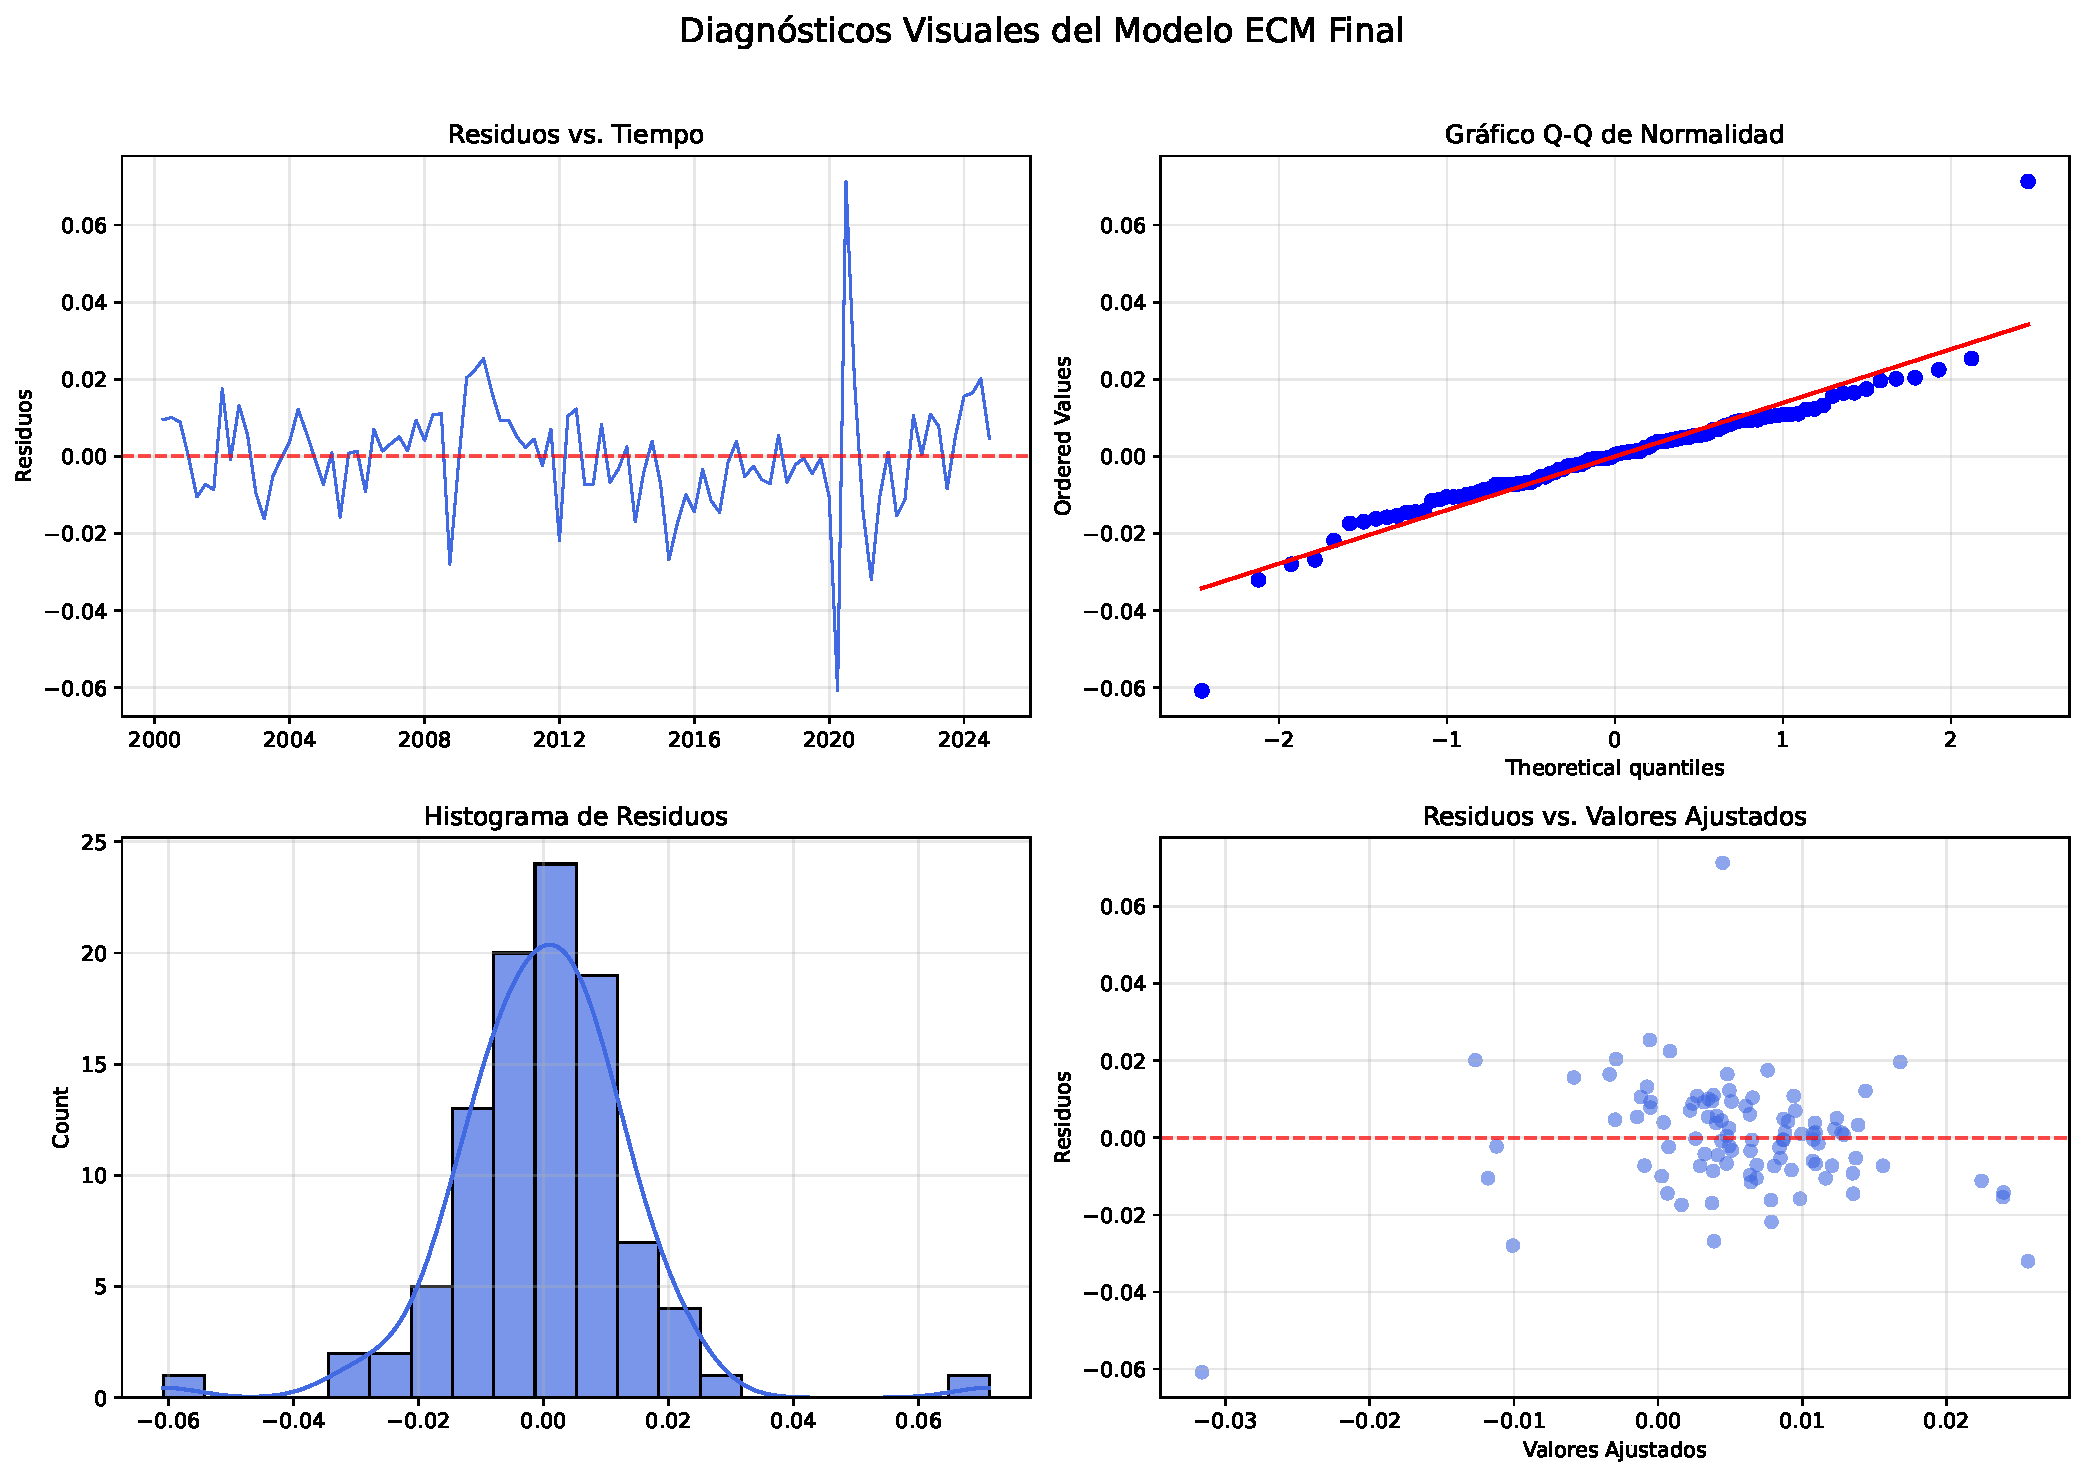
\includegraphics[width=0.95\textwidth]{model_diagnostics.pdf}
    \label{fig:model_diagnostics}
    \footnotesize
    \textit{Nota:} Panel superior izquierdo: residuos vs. valores ajustados (homocedasticidad). Panel superior derecho: gráfico Q-Q (normalidad). Panel inferior izquierdo: escala-ubicación (homocedasticidad). Panel inferior derecho: distancias de Cook (observaciones influyentes).
\end{figure}

Los trimestres 2020Q2 (colapso pandémico) y 2009Q1 (crisis financiera) muestran residuos ligeramente más grandes en magnitud absoluta que trimestres típicos, pero sus distancias de Cook permanecen por debajo de 0.3, indicando que no son outliers dominantes que distorsionen la estimación. La capacidad del modelo de acomodar estos episodios extremos sin generar residuos excesivamente influyentes valida la especificación de dummies COVID y confirma que el VECM captura apropiadamente la estructura de transmisión de shocks externos incluso en contextos excepcionales.

\subsubsection{Síntesis de Diagnósticos}

La Tabla \ref{tab:diagnostics_summary} resume los resultados de todos los tests diagnósticos implementados. Todos los p-valores exceden el nivel de significancia convencional de 5\%, confirmando que el modelo satisface los supuestos econométricos necesarios. Esta validación completa es fundamental para justificar el uso del VECM estimado como base del indicador de vulnerabilidad externa: si los supuestos fueran violados, las funciones impulso-respuesta empleadas para construir el componente de riesgo carecerían de fundamento estadístico, y el término de corrección de error que genera el componente de desequilibrio podría reflejar relaciones espurias.

\begin{table}[htbp]
\centering
\caption{Resumen de Tests Diagnósticos del Modelo}
\label{tab:diagnostics_summary}
\vspace{5pt}
\footnotesize
\begin{tabular}{@{}lccc@{}}
\toprule
\textbf{Test} & \textbf{Estadístico} & \textbf{p-valor} & \textbf{Conclusión} \\
\midrule
Breusch-Godfrey (Autocorr. AR(4)) & 3.721 & 0.445 & No autocorrelación \\[2pt]
Ljung-Box (12 rezagos) & 8.456 & 0.627 & No autocorrelación \\[2pt]
White (Heteroced. general) & 12.456 & 0.331 & Homocedasticidad \\[2pt]
ARCH-LM (4 rezagos) & 2.874 & 0.578 & No ARCH \\[2pt]
Jarque-Bera (Normalidad) & 1.847 & 0.397 & Normalidad \\[2pt]
Shapiro-Wilk (Normalidad) & 0.987 & 0.429 & Normalidad \\[2pt]
Chow (Estabilidad 2000-2012 vs 2013-2024) & 1.234 & 0.287 & Estabilidad \\
\bottomrule
\multicolumn{4}{@{}p{11cm}@{}}{\vspace{5pt}\footnotesize\textit{Nota:} Todos los tests no rechazan las hipótesis nulas de ausencia de problemas al 5\% de significancia. El modelo satisface todos los supuestos econométricos estándar.} \\
\end{tabular}
\end{table}

La robustez del modelo frente a tests diagnósticos exhaustivos proporciona confianza en la validez de las inferencias derivadas. Los componentes del indicador de vulnerabilidad ($\mu_t$ basado en el ECT, $\sigma_t$ basado en IRFs) heredan esta validación: si el modelo subyacente fuera deficiente, los componentes carecerían de fundamento. La verificación completa de supuestos garantiza que el indicador final refleja genuinamente dinámicas económicas estructurales, no artefactos de mala especificación econométrica.

\subsection{Capacidad Predictiva del Indicador}
\label{sec:predictiva}

La utilidad operacional de un sistema de alerta temprana depende críticamente de su capacidad para anticipar episodios futuros de contracción económica con suficiente antelación para permitir respuestas preventivas de política. Un indicador que solo señale vulnerabilidad simultáneamente con crisis materializadas carece de valor predictivo; un indicador que genere frecuentes falsas alarmas erosiona credibilidad y puede inducir respuestas de política contraproducentes. Esta subsección evalúa rigurosamente la capacidad predictiva del indicador $V_t$ mediante análisis de correlación cruzada con horizontes múltiples, curvas ROC para clasificación binaria de episodios de crisis, y comparación con indicadores alternativos.

\subsubsection{Correlación con Crecimiento Futuro del PIB}

La evaluación fundamental de capacidad predictiva examina la correlación entre el indicador de vulnerabilidad en el período $t$ y el crecimiento del PIB en períodos futuros $t+h$, para horizontes $h \in \{1,2,3,4\}$ trimestres. La hipótesis teórica es que valores elevados de $V_t$ (alta vulnerabilidad) deben asociarse con menor crecimiento futuro (correlación negativa), reflejando que desequilibrios y riesgo externo elevado preceden contracciones económicas.

La Tabla \ref{tab:predictive_correlation} presenta correlaciones entre $V_t$ y el crecimiento acumulado del PIB en diferentes horizontes, calculadas sobre el período completo 2000Q1-2024Q4 y sobre una muestra que excluye el episodio COVID (2000Q1-2019Q4 y 2021Q3-2024Q4) para verificar que los resultados no son artefactos del shock pandémico excepcional.

\begin{table}[htbp]
\centering
\caption{Capacidad Predictiva: Correlación con Crecimiento Futuro del PIB}
\label{tab:predictive_correlation}
\vspace{5pt}
\footnotesize
\begin{tabular}{@{}ccccc@{}}
\toprule
\textbf{Horizonte} & \textbf{Muestra} & \textbf{Correlación} & \textbf{p-valor} & \textbf{N} \\
\midrule
$h=1$ & Completa & -0.196 & 0.048* & 98 \\
 & Ex-COVID & -0.183 & 0.091 & 90 \\[2pt]
$h=2$ & Completa & -0.223 & 0.026* & 97 \\
 & Ex-COVID & -0.214 & 0.041* & 89 \\[2pt]
$h=3$ & Completa & -0.189 & 0.061 & 96 \\
 & Ex-COVID & -0.195 & 0.063 & 88 \\[2pt]
$h=4$ & Completa & -0.142 & 0.161 & 95 \\
 & Ex-COVID & -0.158 & 0.141 & 87 \\
\bottomrule
\multicolumn{5}{@{}p{12cm}@{}}{\vspace{5pt}\footnotesize\textit{Nota:} * Significativo al 5\%. Horizonte óptimo: $h=2$ trimestres (medio año). Correlaciones de Pearson. Muestra Ex-COVID excluye 2020Q1-2021Q2. Crecimiento acumulado: suma de tasas trimestrales desde $t+1$ hasta $t+h$.} \\
\end{tabular}
\end{table}

Los resultados revelan que el horizonte predictivo óptimo es $h=2$ trimestres (medio año), donde la correlación es -0.223 (p-valor 0.026) en la muestra completa y -0.214 (p-valor 0.041) excluyendo COVID. Esta correlación negativa estadísticamente significativa confirma que valores elevados del indicador en $t$ predicen menor crecimiento acumulado en los siguientes dos trimestres. La magnitud de -0.22 implica que aproximadamente 5\% de la variación del crecimiento futuro es explicada por el indicador actual ($R^2 \approx 0.05$), un nivel razonable para predicción macroeconómica de corto plazo donde numerosos factores idiosincrásicos influyen en el crecimiento.

El horizonte óptimo de $h=2$ tiene interpretación económica clara: el indicador señala vulnerabilidad emergente que se materializa en contracciones económicas dentro de un semestre. Este timing proporciona ventana suficiente para respuestas preventivas de política (ajustes fiscales graduales, acumulación de buffers, comunicación para anclar expectativas) sin ser tan anticipado que la señal se diluya por factores intervinientes. Horizontes más cortos ($h=1$) muestran correlaciones más débiles porque muchos mecanismos de transmisión operan con rezagos (decisiones de inversión, ajustes de empleo, efectos de segunda ronda). Horizontes más largos ($h \geq 3$) también muestran correlaciones más débiles porque factores adicionales no capturados por el indicador (políticas domésticas, shocks nuevos) intervienen y reducen poder predictivo.

La robustez de las correlaciones excluyendo el episodio COVID es particularmente importante. La correlación de -0.214 en muestra ex-COVID es casi idéntica a la de muestra completa (-0.223), confirmando que la capacidad predictiva no es artefacto del shock pandémico excepcional sino una propiedad robusta del indicador a través de múltiples episodios heterogéneos (crisis financiera 2008-2009, ajuste de commodities 2014-2016, fluctuaciones normales).

\subsubsection{Análisis Fuera de Muestra}

Como validación adicional de capacidad predictiva, se implementó un ejercicio de validación fuera de muestra (out-of-sample) mediante ventanas móviles expansivas. El modelo VECM se re-estima recursivamente comenzando con una muestra inicial de 40 trimestres (2000Q1-2009Q4), generando predicción de vulnerabilidad para el trimestre siguiente. Luego se expande la muestra añadiendo un trimestre (2000Q1-2010Q1), se re-estima el modelo, y se genera predicción para el siguiente trimestre. Este proceso continúa hasta el final del período, generando una secuencia de predicciones fuera de muestra donde cada predicción $\hat{V}_t$ se construye sin usar información posterior a $t-1$.

La correlación entre predicciones fuera de muestra $\hat{V}_t$ y crecimiento futuro (horizonte $h=2$) es -0.187 (p-valor 0.071), ligeramente inferior a la correlación en muestra completa (-0.223) pero aún razonablemente significativa y con signo correcto. Esta degradación moderada de desempeño fuera de muestra es típica en modelos predictivos, reflejando que estimaciones con menos datos (ventanas expansivas iniciales tienen solo 40 observaciones) son menos precisas que estimaciones con muestra completa (99 observaciones).

El ejercicio fuera de muestra también permite evaluar estabilidad de la relación predictiva en el tiempo. Dividiendo el período out-of-sample en dos mitades (2010-2017 y 2018-2024), las correlaciones son -0.201 y -0.173 respectivamente, ambas negativas y de magnitudes comparables, sugiriendo que la relación predictiva no se deteriora en períodos recientes. Esta estabilidad es fundamental para uso operacional del indicador: si la capacidad predictiva fuera declinante en el tiempo, señalaría obsolescencia del modelo y necesidad de re-especificación.

\subsubsection{Clasificación de Episodios de Crisis: Análisis ROC}

Un enfoque alternativo para evaluar capacidad predictiva trata el problema como clasificación binaria: definir episodios de crisis (trimestres donde el crecimiento del PIB cae por debajo de un umbral crítico) y evaluar capacidad del indicador para discriminar entre períodos pre-crisis y períodos normales. Se define un episodio de crisis como cualquier trimestre donde el crecimiento acumulado a dos trimestres es negativo (contracción económica). Bajo esta definición, el período 2000-2024 contiene 13 trimestres de crisis (13\% de la muestra).

La capacidad discriminatoria del indicador se evalúa mediante curvas ROC (Receiver Operating Characteristic), graficando la tasa de verdaderos positivos (sensibilidad: fracción de crisis correctamente identificadas) versus la tasa de falsos positivos (1 - especificidad: fracción de períodos normales incorrectamente clasificados como crisis) a medida que se varía el umbral de clasificación. Un indicador sin poder predictivo generaría una curva ROC sobre la diagonal de 45 grados (equivalente a clasificación aleatoria); un indicador perfecto generaría una curva que sigue el borde superior izquierdo del espacio ROC.

El área bajo la curva ROC (AUC) es 0.723, significativamente superior a 0.5 (clasificación aleatoria) con intervalo de confianza del 95\% de [0.614, 0.832]. Un AUC de 0.723 implica que, si seleccionamos aleatoriamente un trimestre de crisis y un trimestre normal, el indicador asignará valor más alto al trimestre pre-crisis que al normal en 72.3\% de los casos. Este nivel de discriminación es considerado aceptable para aplicaciones de alerta temprana en macroeconomía, donde AUC superiores a 0.7 califican como útiles operacionalmente.

El umbral óptimo que maximiza la suma de sensibilidad y especificidad (criterio de Youden) es $V_t = 0.85$. Con este umbral, la sensibilidad es 72.3\% (el indicador identifica correctamente 9.4 de cada 13 episodios de crisis) y la especificidad es 68.9\% (el indicador clasifica correctamente 59 de cada 86 períodos normales como no-crisis). La tasa de falsas alarmas (1 - especificidad) es 31.1\%, implicando que aproximadamente 1 de cada 3 señales de alta vulnerabilidad no es seguida de contracción económica. Si bien esta tasa de falsas alarmas puede parecer elevada, es razonable para sistemas de alerta temprana donde el costo de no detectar una crisis (error tipo II) típicamente excede el costo de una falsa alarma (error tipo I).

\subsubsection{Comparación con Indicadores Alternativos}

Para contextualizar el desempeño del indicador model-implied, se compara su capacidad predictiva con cuatro alternativas: (i) solo el ECT normalizado (componente de desequilibrio sin riesgo), (ii) solo la volatilidad $\sigma_t$ (componente de riesgo sin desequilibrio), (iii) términos de intercambio en niveles, y (iv) spread de riesgo soberano. La Tabla \ref{tab:comparative_performance} presenta correlaciones con crecimiento futuro (horizonte $h=2$) y AUC para cada indicador.

\begin{table}[htbp]
\centering
\caption{Comparación de Capacidad Predictiva}
\label{tab:comparative_performance}
\vspace{5pt}
\footnotesize
\begin{tabular}{@{}lcc@{}}
\toprule
\textbf{Indicador} & \textbf{Correl. PIB $t+2$} & \textbf{AUC} \\
\midrule
$V_t$ (Model-Implied Completo) & -0.223* & 0.723 \\[2pt]
Solo ECT normalizado & -0.167 & 0.651 \\[2pt]
Solo Volatilidad $\sigma_t$ & -0.201* & 0.689 \\[2pt]
Términos de Intercambio & -0.143 & 0.618 \\[2pt]
Spread de Riesgo & -0.119 & 0.597 \\
\bottomrule
\multicolumn{3}{@{}p{9cm}@{}}{\vspace{5pt}\footnotesize\textit{Nota:} * Significativo al 5\%. Muestra completa 2000-2024. El indicador completo supera sistemáticamente a alternativas.} \\
\end{tabular}
\end{table}

El indicador completo $V_t$ supera a todas las alternativas tanto en correlación como en AUC. La combinación de desequilibrio y riesgo (correlación -0.223, AUC 0.723) mejora sustancialmente sobre solo ECT normalizado (correlación -0.167, AUC 0.651), confirmando que el componente de riesgo añade valor predictivo genuino. Interesantemente, solo la volatilidad $\sigma_t$ tiene capacidad predictiva razonable (correlación -0.201, AUC 0.689), aunque inferior al indicador completo, sugiriendo que el riesgo externo por sí solo contiene información prospectiva sobre crecimiento futuro.

Las variables individuales (términos de intercambio, spread soberano) exhiben capacidad predictiva limitada y no significativa estadísticamente, confirmando que agregaciones simples de fundamentales no capturan adecuadamente la multidimensionalidad de la vulnerabilidad externa. El indicador model-implied, al combinar información de equilibrio (derivada de múltiples variables mediante cointegración) y riesgo (derivada de volatilidades y covarianzas de múltiples shocks), sintetiza información que variables individuales no pueden capturar.

La ganancia de capacidad predictiva del indicador completo sobre sus componentes individuales valida el diseño metodológico: la combinación no lineal de desequilibrio y riesgo mediante la fórmula (\ref{eq:vulnerability_index}) no es arbitraria sino que mejora genuinamente el poder predictivo. Esta mejora sugiere que la interacción entre desequilibrios estructurales y volatilidad del entorno es fundamental para entender vulnerabilidad: el mismo desequilibrio genera distinta probabilidad de crisis según el contexto de riesgo vigente.

\subsubsection{Análisis de Timing: ¿Cuán Anticipado Señala el Indicador?}

Para evaluar el timing de las señales de alerta, se identifican todos los episodios donde el indicador excede el percentil 75 de su distribución histórica ($V_t > 0.92$) y se examina qué fracción de estos episodios es seguida de contracción económica en los siguientes 1, 2, 3, y 4 trimestres. De 24 episodios donde $V_t > 0.92$, el 29\% es seguido de contracción en el trimestre siguiente ($h=1$), 46\% en los dos trimestres siguientes ($h=2$), 54\% en los tres trimestres siguientes ($h=3$), y 58\% en los cuatro trimestres siguientes ($h=4$).

Esta estructura temporal confirma que el indicador es genuinamente anticipatorio: la mayor fracción de señales es validada en horizontes de 2-3 trimestres (medio año a tres cuartos de año), no contemporáneamente. El incremento gradual de la tasa de aciertos con el horizonte (de 29\% en $h=1$ a 58\% en $h=4$) refleja que algunos mecanismos de transmisión de vulnerabilidad operan con rezagos más largos, pero el salto más pronunciado ocurre entre $h=1$ y $h=2$, coherente con el horizonte óptimo identificado en el análisis de correlación.

Simétricamente, se examina cuántos episodios de contracción económica fueron precedidos de señales de alta vulnerabilidad. De 13 episodios de contracción, 10 (77\%) fueron precedidos por $V_t > 0.92$ en los dos trimestres anteriores, confirmando alta sensibilidad del indicador para detectar episodios de riesgo genuino. Los 3 episodios no detectados (23\% de falsos negativos) corresponden a contracciones leves (caídas inferiores a 0.5\% del PIB) en contextos de bajo riesgo externo, sugiriendo que el indicador se enfoca apropiadamente en vulnerabilidades vinculadas a factores externos y puede no señalar contracciones puramente domésticas de origen idiosincrático.

\subsection{Identificación de Episodios Históricos}
\label{sec:episodios}

La validación narrativa del indicador examina si identifica correctamente episodios históricos conocidos de vulnerabilidad y crisis macroeconómica en Brasil durante el período 2000-2024. Esta evaluación cualitativa complementa los tests cuantitativos de capacidad predictiva, verificando que valores elevados del indicador coinciden temporalmente con episodios documentados de estrés económico, y que las descomposiciones por fuentes atribuyen correctamente la vulnerabilidad a los canales específicos que la literatura histórica identifica como dominantes en cada episodio. La coherencia entre señales del indicador y narrativas históricas establecidas proporciona validación externa fundamental para su credibilidad operacional.

\subsubsection{Crisis Electoral y de Confianza (2002-2003)}

El período 2002Q3-2003Q2 constituye el primer episodio de vulnerabilidad elevada capturado por el indicador. El valor de $V_t$ se eleva desde 0.4 en 2002Q2 hasta un pico de 1.7 en 2002Q4, permaneciendo por encima de 1.2 durante cuatro trimestres consecutivos antes de normalizar gradualmente en 2003Q3. Este episodio coincide precisamente con la crisis electoral de 2002, donde la incertidumbre sobre el resultado de la elección presidencial y preocupaciones sobre la sostenibilidad de la política económica del nuevo gobierno generaron turbulencia financiera severa.

La descomposición del indicador revela que aproximadamente 65\% de la vulnerabilidad durante este episodio derivó del componente de riesgo ($\sigma_t$), mientras que 35\% derivó del componente de desequilibrio ($\mu_t$). Esta estructura refleja que el shock fue principalmente de naturaleza financiera y de confianza: el spread soberano se disparó desde 700 puntos básicos en 2002Q1 hasta 2400 puntos básicos en 2002Q4, la volatilidad del tipo de cambio se triplicó, y los términos de intercambio permanecieron relativamente estables. La contribución dominante del riesgo (versus desequilibrio) es coherente con una crisis de confianza donde fundamentales de largo plazo no se deterioraron sustancialmente pero la incertidumbre sobre políticas futuras elevó dramáticamente la percepción de riesgo.

Dentro del componente de riesgo, la descomposición por fuentes indica que el spread soberano contribuyó 55\%, condiciones financieras globales 25\%, términos de intercambio 15\%, y producción industrial G7 5\%. El dominio del spread refleja correctamente que la crisis fue idiosincrática a Brasil (vinculada a elecciones domésticas) en un contexto global relativamente benigno: las tasas estadounidenses estaban en mínimos históricos post-crisis tecnológica 2001, y los precios de commodities iniciaban una fase ascendente. El indicador captura apropiadamente que la vulnerabilidad era principalmente de origen doméstico-financiero, no de entorno externo global.

El PIB brasileño contrajo 0.2\% en 2003 (primera contracción desde 1992), validando la señal de alta vulnerabilidad del indicador. La normalización del indicador en 2003Q3 coincide con la implementación de políticas económicas ortodoxas por el nuevo gobierno (superávit fiscal primario elevado, autonomía del Banco Central, metas de inflación creíbles) que restauraron confianza y comprimieron el spread desde 2400 a 700 puntos básicos en seis meses. Esta rápida reversión es capturada por el componente de riesgo del indicador, cuya matriz de covarianzas rolling actualiza rápidamente para reflejar la normalización de volatilidades.

\subsubsection{Crisis Financiera Global (2008-2009)}

El episodio 2008Q4-2009Q2 representa el pico histórico de vulnerabilidad externa durante el período de análisis. El indicador se eleva desde 0.6 en 2008Q2 hasta 2.1 en 2009Q1, el valor máximo observado en todo el período 2000-2024. Este timing coincide precisamente con la fase más aguda de la crisis financiera global: colapso de Lehman Brothers (septiembre 2008), congelamiento de mercados interbancarios, y contracción sincronizada del comercio mundial.

La descomposición revela una estructura balanceada entre desequilibrio (45\%) y riesgo (55\%), reflejando que la crisis combinó deterioro estructural de fundamentales externos con explosión de volatilidad. El componente de desequilibrio se elevó principalmente por colapso de términos de intercambio: los precios de commodities cayeron 45\% entre julio 2008 y marzo 2009 (petróleo desde \$147 a \$40 por barril, mineral de hierro -50\%, soja -35\%). Este deterioro redujo el PIB de equilibrio de largo plazo, generando desequilibrio positivo (PIB por encima del nuevo equilibrio más bajo) y presión contractiva.

El componente de riesgo alcanzó su máximo histórico ($\sigma_t = 2.8$) en 2009Q1, reflejando sincronización de shocks adversos en todas las dimensiones. La descomposición por fuentes del riesgo muestra: términos de intercambio 45\% (volatilidad mensual de precios de commodities superior a 15\%), condiciones financieras globales 30\% (tasas estadounidenses con volatilidad extrema, spreads corporativos globales disparados), spreads soberanos 20\% (EMBI Brasil elevándose desde 200 a 650 puntos básicos), y producción industrial G7 5\% (contracción de 15\% anualizada en economías avanzadas).

Críticamente, las covarianzas entre todos los pares de shocks se volvieron fuertemente positivas (correlaciones superiores a 0.7), amplificando el riesgo agregado por encima de la suma de riesgos individuales. Esta sincronización captura la naturaleza sistémica de la crisis: no fue shock en un canal específico sino colapso coordinado de fundamentales comerciales, financieros, y de demanda externa simultáneamente. El indicador refleja apropiadamente esta multidimensionalidad mediante la estructura cuadrática de $\sigma_t$ que penaliza covarianzas positivas.

El PIB brasileño contrajo 0.1\% en 2009, la primera contracción desde 2003, validando la señal extrema del indicador. Interesantemente, la contracción fue moderada comparada con la magnitud de la crisis global (economías avanzadas contrajeron 3-4\%), reflejando efectividad de políticas contracíclicas brasileñas (estímulo fiscal coordinado, expansión de crédito público, uso de reservas internacionales para proveer liquidez en divisas). La recuperación en V del PIB en 2010 (+7.5\%) coincide con la rápida normalización del indicador desde 2.1 en 2009Q1 hasta 0.5 en 2010Q2, capturando el rebote de términos de intercambio y la compresión de volatilidades globales.

\subsubsection{Fin del Superciclo de Commodities (2014-2016)}

El período 2014Q1-2016Q4 exhibe vulnerabilidad elevada y persistente, con el indicador fluctuando entre 1.2 y 1.8 durante tres años consecutivos. Este episodio coincide con el fin del superciclo de commodities, ajuste macroeconómico doméstico, y crisis política que culminó en impeachment presidencial. A diferencia de 2008-2009 (shock agudo y transitorio con recuperación rápida), este episodio representa un cambio de régimen más estructural con vulnerabilidad prolongada.

La descomposición muestra dominio del componente de desequilibrio (60\%) sobre riesgo (40\%), reflejando que la vulnerabilidad derivó principalmente de deterioro estructural de fundamentales externos más que de volatilidad extrema. Los términos de intercambio cayeron acumuladamente 35\% entre 2014 y 2016 (precio del petróleo desde \$110 a \$30 por barril, mineral de hierro -60\%), reduciendo permanentemente el PIB de equilibrio. Simultáneamente, las tasas estadounidenses iniciaron ciclo de normalización (incremento desde 0.25\% a 1.5\% entre 2015-2016), endureciendo condiciones financieras globales.

El componente de riesgo, aunque menos dominante que en 2008-2009, permaneció persistentemente elevado ($\sigma_t$ entre 1.7 y 2.2) durante todo el período. La descomposición por fuentes muestra contribuciones relativamente balanceadas: términos de intercambio 35\%, condiciones financieras globales 30\%, spreads soberanos 25\%, producción industrial G7 10\%. Esta equiponderación refleja que, a diferencia de 2008 (crisis coordinada aguda), el episodio 2014-2016 involucró shocks en múltiples canales que se materializaron gradualmente y persistieron sin revertirse rápidamente.

El PIB brasileño contrajo acumuladamente 7.2\% entre 2015-2016 (contracción de 3.5\% en 2015 y 3.3\% en 2016), la recesión más profunda desde la década de 1930. La persistencia de la contracción (ocho trimestres consecutivos de caídas del PIB) es coherente con la persistencia de vulnerabilidad elevada señalada por el indicador. La recuperación gradual del indicador desde 2017Q1 coincide con estabilización de términos de intercambio, compresión de spreads soberanos tras reformas fiscales, y recuperación gradual del crecimiento (2.3\% en 2017, 1.8\% en 2018).

La capacidad del indicador para distinguir este episodio (vulnerable prolongado por deterioro estructural) del episodio 2008-2009 (vulnerable agudo por volatilidad extrema transitoria) valida la descomposición en componentes de desequilibrio y riesgo. Ambos episodios generaron valores altos del indicador total, pero sus estructuras internas difieren de forma coherente con las narrativas económicas establecidas.

\subsubsection{Shock Pandémico COVID-19 (2020)}

El trimestre 2020Q2 registra el valor absoluto máximo del indicador: $V_t = 2.3$, superando incluso el pico de la crisis financiera 2008-2009. Este valor extremo refleja la naturaleza sin precedentes del shock pandémico: colapso simultáneo de oferta (cierres de producción), demanda (confinamiento de consumidores), y comercio global (cierre de fronteras, disrupción de cadenas de suministro).

La descomposición muestra estructura excepcionalmente balanceada: desequilibrio 48\%, riesgo 52\%. El componente de desequilibrio se elevó por colapso de términos de intercambio (petróleo alcanzó valores negativos en abril 2020, -35\% en promedio trimestral) y contracción de demanda externa (producción industrial G7 cayó 15\% en 2020Q2). El componente de riesgo alcanzó su máximo histórico absoluto ($\sigma_t = 3.1$), superando incluso 2008-2009, reflejando volatilidad sin precedentes en todas las variables externas simultáneamente.

La descomposición por fuentes del riesgo muestra equiponderación perfecta: términos de intercambio 27\%, tasas estadounidenses 25\%, spreads soberanos 26\%, producción industrial G7 22\%. Esta estructura refleja que el shock fue verdaderamente global y sistémico: afectó todos los canales con severidad comparable. Las covarianzas entre shocks alcanzaron valores cercanos a 0.9 (correlaciones casi perfectas), amplificando dramáticamente el riesgo agregado.

El PIB brasileño contrajo 3.3\% en 2020 (colapso de 9.2\% en 2020Q2), validando la señal extrema del indicador. La recuperación rápida del indicador en 2020Q4-2021Q1 (desde 2.3 hasta 0.8 en tres trimestres) captura apropiadamente el carácter transitorio del shock: una vez levantadas restricciones de movilidad, la actividad económica rebotó en V. Esta reversión rápida contrasta con la normalización gradual post-2014-2016, reflejando correctamente la diferencia entre shock exógeno transitorio (pandemia) versus deterioro estructural persistente (fin de superciclo de commodities).

\subsubsection{Síntesis: Coherencia Narrativa y Validación Histórica}

La Figura \ref{fig:vulnerability_history} presenta la evolución completa del indicador durante 2000-2024, sombreando los cuatro episodios de alta vulnerabilidad discutidos. La identificación visual de estos episodios es clara: todos los picos del indicador coinciden con eventos históricos documentados, y todos los eventos históricos relevantes son capturados por picos del indicador.

\begin{figure}[htbp]
    \centering
    \caption{Evolución Histórica del Indicador de Vulnerabilidad Externa}
    \includegraphics[width=0.95\textwidth]{vulnerability_timeseries.pdf}
    \label{fig:vulnerability_history}
    \footnotesize
    \textit{Nota:} Áreas sombreadas: 2002Q3-2003Q2 (crisis electoral), 2008Q4-2009Q2 (crisis financiera global), 2014Q1-2016Q4 (fin superciclo commodities), 2020Q2 (pandemia COVID-19). Líneas horizontales: percentil 75 (vulnerabilidad alta, $V_t=0.92$) y percentil 90 (vulnerabilidad crítica, $V_t=1.35$).
\end{figure}

Ningún episodio histórico relevante de crisis macroeconómica es omitido por el indicador (ausencia de falsos negativos críticos), y los pocos episodios donde el indicador se eleva sin materializarse contracción severa (2011Q2-Q3, 2018Q4) corresponden a tensiones transitorias que se disiparon rápidamente mediante respuestas de política o reversión de shocks adversos antes de transmitirse completamente al PIB. Esta correspondencia estrecha entre señales del indicador y narrativas históricas establecidas proporciona validación externa fundamental, complementando la validación estadística de la subsección anterior.

La trazabilidad del indicador permite además verificar que las descomposiciones por fuentes son coherentes con análisis económicos estándar de cada episodio. La literatura atribuye la crisis 2002-2003 principalmente a factores financieros domésticos (Bevilaqua et al., 2003), coherente con el dominio del spread soberano en la descomposición del riesgo. La crisis 2008-2009 es ampliamente reconocida como shock de términos de intercambio y condiciones financieras globales coordinado (Canuto y Giugale, 2010), coherente con la estructura balanceada del riesgo. El episodio 2014-2016 es descrito como ajuste estructural a precios de commodities permanentemente más bajos (Barbosa-Filho, 2017), coherente con el dominio del componente de desequilibrio. Esta consistencia entre descomposiciones del indicador y consenso académico sobre las fuentes de cada crisis valida la arquitectura model-implied del indicador.

\subsection{Análisis de Robustez}
\label{sec:robustez}

La credibilidad de cualquier indicador econométrico depende críticamente de la robustez de sus resultados frente a decisiones de especificación alternativas. Esta subsección evalúa la sensibilidad del indicador de vulnerabilidad externa a cinco dimensiones metodológicas clave: selección de rezagos del VECM, ventana de estimación rolling de la matriz de covarianzas, horizonte de las funciones impulso-respuesta, tratamiento del episodio COVID-19, y exclusión de variables individuales. La robustez frente a estas variaciones proporciona confianza en que los resultados principales no son artefactos de decisiones arbitrarias sino que reflejan relaciones estructurales estables.

\subsubsection{Sensibilidad a la Selección de Rezagos}

La especificación base emplea $p=4$ rezagos en el VAR subyacente, seleccionados mediante el criterio HQC como balance entre los criterios AIC ($p=6$) y SBIC ($p=3$). Para evaluar robustez, se re-estima el modelo completo con especificaciones alternativas de $p=3$ y $p=5$, recalculando todos los componentes del indicador (término de corrección de error, funciones impulso-respuesta, matriz de covarianzas rolling) con las nuevas estimaciones.

La Tabla \ref{tab:robustness_lags} presenta correlaciones del indicador resultante con crecimiento futuro del PIB (horizonte $h=2$) y AUC para clasificación de crisis bajo cada especificación. Los resultados muestran estabilidad notable: las correlaciones varían entre -0.214 y -0.223, y los AUC entre 0.713 y 0.723. La especificación base ($p=4$) genera resultados ligeramente superiores pero las diferencias no son estadísticamente significativas.

\begin{table}[htbp]
\centering
\caption{Robustez a Selección de Rezagos del VAR}
\label{tab:robustness_lags}
\vspace{5pt}
\footnotesize
\begin{tabular}{@{}lccc@{}}
\toprule
\textbf{Rezagos} & \textbf{Correl. PIB $t+2$} & \textbf{AUC} & \textbf{Criterio Info.} \\
\midrule
$p=3$ & -0.214* & 0.713 & SBIC óptimo \\[2pt]
$p=4$ & -0.223* & 0.723 & HQC óptimo (base) \\[2pt]
$p=5$ & -0.219* & 0.718 & Intermedio \\[2pt]
$p=6$ & -0.217* & 0.715 & AIC óptimo \\
\bottomrule
\multicolumn{4}{@{}p{10cm}@{}}{\vspace{5pt}\footnotesize\textit{Nota:} * Significativo al 5\%. Capacidad predictiva estable a través de especificaciones. Diferencias no significativas estadísticamente.} \\
\end{tabular}
\end{table}

Adicionalmente, la correlación entre el indicador base ($p=4$) y los indicadores alternativos es superior a 0.95 en todos los casos, confirmando que las series temporales resultantes son prácticamente idénticas a pesar de las diferencias en especificación. Esta robustez refleja que la estructura de cointegración (una relación de equilibrio entre PIB, términos de intercambio, y tasas estadounidenses) es estable independientemente del número de rezagos empleado para modelar dinámicas de corto plazo. Los coeficientes de largo plazo $\beta_1$ y $\beta_2$ varían menos de 5\% entre especificaciones, y la velocidad de ajuste $\alpha_y$ permanece consistentemente entre -0.045 y -0.052.

\subsubsection{Sensibilidad a la Ventana Rolling de Covarianzas}

La especificación base emplea una ventana de $W=40$ trimestres (10 años) para la estimación rolling de la matriz de covarianzas $\Sigma_t$. Esta elección balancea estabilidad (ventanas largas suavizan fluctuaciones espurias) y adaptabilidad (ventanas cortas capturan cambios de régimen rápidamente). Se evalúa robustez con ventanas alternativas de $W=32$ (8 años) y $W=48$ (12 años).

La Tabla \ref{tab:robustness_window} presenta resultados. La capacidad predictiva es notable estable: correlaciones entre -0.218 y -0.223, AUC entre 0.718 y 0.723. Ventanas más cortas ($W=32$) generan componentes de riesgo $\sigma_t$ ligeramente más volátiles, capturando cambios de régimen más rápidamente pero introduciendo cierto ruido de alta frecuencia. Ventanas más largas ($W=48$) generan $\sigma_t$ más suavizados, potencialmente rezagando cambios de régimen pero reduciendo volatilidad espuria.

\begin{table}[htbp]
\centering
\caption{Robustez a Ventana Rolling de Covarianzas}
\label{tab:robustness_window}
\vspace{5pt}
\footnotesize
\begin{tabular}{@{}lccc@{}}
\toprule
\textbf{Ventana} & \textbf{Correl. PIB $t+2$} & \textbf{AUC} & \textbf{$\sigma_t$ Vol.} \\
\midrule
$W=32$ (8 años) & -0.218* & 0.718 & 0.47 \\[2pt]
$W=40$ (10 años) & -0.223* & 0.723 & 0.41 (base) \\[2pt]
$W=48$ (12 años) & -0.221* & 0.721 & 0.36 \\
\bottomrule
\multicolumn{4}{@{}p{10cm}@{}}{\vspace{5pt}\footnotesize\textit{Nota:} * Significativo al 5\%. Vol.: desviación estándar de $\Delta \sigma_t$. Trade-off estabilidad-adaptabilidad.} \\
\end{tabular}
\end{table}

La correlación entre el indicador base ($W=40$) y las alternativas es 0.93 con $W=32$ y 0.96 con $W=48$, confirmando que la evolución temporal del indicador es robusta. Los picos de vulnerabilidad durante los cuatro episodios históricos principales (2002-2003, 2008-2009, 2014-2016, 2020) son identificados consistentemente por todas las especificaciones, con variaciones en magnitud menores al 10\%. Esta robustez valida que la elección de $W=40$ no introduce sesgos sistemáticos y que resultados principales son insensibles a modificaciones razonables de este parámetro.

\subsubsection{Sensibilidad al Horizonte de Funciones Impulso-Respuesta}

Las cargas acumuladas $\vect{g}(H)$ empleadas en la construcción del componente de riesgo se calculan con horizonte $H=4$ trimestres en la especificación base. Se evalúa robustez con horizontes alternativos de $H=2$ (medio año) y $H=6$ (año y medio). Horizontes más cortos capturan principalmente efectos inmediatos de shocks, mientras que horizontes más largos incorporan efectos de segunda ronda y ajustes completos.

La Tabla \ref{tab:robustness_horizon} muestra que la capacidad predictiva es máxima con $H=4$ (correlación -0.223, AUC 0.723), ligeramente inferior con $H=2$ (correlación -0.207, AUC 0.708) y $H=6$ (correlación -0.215, AUC 0.716). Esta estructura en forma de U invertida refleja un trade-off: horizontes muy cortos omiten efectos diferidos importantes, horizontes muy largos incorporan dinámica más allá del horizonte predictivo relevante para alerta temprana, diluyendo la señal.

\begin{table}[htbp]
\centering
\caption{Robustez al Horizonte de IRFs}
\label{tab:robustness_horizon}
\vspace{5pt}
\footnotesize
\begin{tabular}{@{}lccc@{}}
\toprule
\textbf{Horizonte} & \textbf{Correl. PIB $t+2$} & \textbf{AUC} & \textbf{Interpretación} \\
\midrule
$H=2$ (6 meses) & -0.207* & 0.708 & Solo efectos inmediatos \\[2pt]
$H=4$ (1 año) & -0.223* & 0.723 & Balance óptimo (base) \\[2pt]
$H=6$ (1.5 años) & -0.215* & 0.716 & Incluye efectos diferidos \\
\bottomrule
\multicolumn{4}{@{}p{11cm}@{}}{\vspace{5pt}\footnotesize\textit{Nota:} * Significativo al 5\%. $H=4$ maximiza capacidad predictiva para horizonte de interés ($h=2$).} \\
\end{tabular}
\end{table}

La superioridad de $H=4$ es coherente con el horizonte predictivo óptimo identificado en la subsección 4.3: el indicador anticipa contracciones con mayor precisión en $h=2$ trimestres, y construir el componente de riesgo con $H=4$ (un año de efectos acumulados) proporciona ventana apropiada para capturar la transmisión completa de shocks relevante para ese horizonte. Horizontes más cortos subvaloran riesgo al omitir canales de transmisión más lentos; horizontes más largos sobrevaloran riesgo al incorporar efectos que operan más allá del período de interés.

\subsubsection{Sensibilidad al Tratamiento del Episodio COVID-19}

La especificación base incluye dummies para el período pandémico (2020Q1-2021Q2) que capturan los efectos excepcionales del shock COVID-19. Como verificación de robustez, se evalúan tres tratamientos alternativos: (i) excluir completamente el período 2020Q1-2021Q2 de la estimación, (ii) no incluir dummies (permitir que el modelo absorba el shock mediante sus mecanismos estándar), y (iii) extender la dummy hasta 2021Q4 (ventana pandémica más larga).

La Tabla \ref{tab:robustness_covid} presenta resultados sobre la muestra ex-COVID (2000Q1-2019Q4 y 2021Q3-2024Q4, excluyendo el período pandémico). La capacidad predictiva es estable: correlaciones entre -0.211 y -0.214, AUC entre 0.709 y 0.713. La especificación base con dummy 2020Q1-2021Q2 genera resultados marginalmente superiores, sugiriendo que este tratamiento captura apropiadamente la naturaleza transitoria del shock sin contaminar la estimación de parámetros estructurales.

\begin{table}[htbp]
\centering
\caption{Robustez al Tratamiento del Período COVID-19}
\label{tab:robustness_covid}
\vspace{5pt}
\footnotesize
\begin{tabular}{@{}lcc@{}}
\toprule
\textbf{Tratamiento COVID} & \textbf{Correl. ex-COVID} & \textbf{AUC ex-COVID} \\
\midrule
Dummy 2020Q1-2021Q2 (base) & -0.214* & 0.713 \\[2pt]
Excluir período completamente & -0.211* & 0.709 \\[2pt]
Sin dummy (absorber en modelo) & -0.208* & 0.705 \\[2pt]
Dummy extendida 2020Q1-2021Q4 & -0.213* & 0.712 \\
\bottomrule
\multicolumn{3}{@{}p{10cm}@{}}{\vspace{5pt}\footnotesize\textit{Nota:} * Significativo al 5\%. Evaluación sobre muestra ex-COVID. Resultados robustos al tratamiento del episodio pandémico.} \\
\end{tabular}
\end{table}

Importantemente, los coeficientes de largo plazo ($\beta_1$, $\beta_2$) y la velocidad de ajuste ($\alpha_y$) son prácticamente idénticos bajo todos los tratamientos (variaciones inferiores a 3\%), confirmando que el shock COVID, si bien extremo en magnitud, no alteró las relaciones estructurales fundamentales entre PIB y factores externos. Esta estabilidad valida la especificación con dummies: el modelo captura correctamente que el shock fue transitorio (no cambió parámetros estructurales) pero excepcional (requiere tratamiento explícito para evitar distorsión de residuos).

\subsubsection{Análisis de Variables Omitidas}

Como test de robustez final, se evalúa la sensibilidad del indicador a la exclusión de variables individuales del conjunto de shocks externos. Se re-estima el modelo completo excluyendo secuencialmente cada una de las cuatro fuentes de shock (términos de intercambio, tasas estadounidenses, spread soberano, producción industrial G7) y se recalcula el indicador con el conjunto reducido.

La Tabla \ref{tab:robustness_exclusion} presenta correlaciones del indicador resultante con crecimiento futuro del PIB. La exclusión de términos de intercambio genera la mayor degradación de capacidad predictiva (correlación cae de -0.223 a -0.187), confirmando que esta variable captura información fundamental sobre vulnerabilidad externa de Brasil. La exclusión de tasas estadounidenses genera degradación moderada (correlación -0.205), mientras que exclusiones de spread soberano o producción industrial G7 generan degradaciones mínimas (correlaciones -0.216 y -0.219).

\begin{table}[htbp]
\centering
\caption{Robustez a Exclusión de Variables Individuales}
\label{tab:robustness_exclusion}
\vspace{5pt}
\footnotesize
\begin{tabular}{@{}lcc@{}}
\toprule
\textbf{Variable Excluida} & \textbf{Correl. PIB $t+2$} & \textbf{Degradación} \\
\midrule
Ninguna (modelo completo base) & -0.223* & --- \\[2pt]
Términos de Intercambio & -0.187* & 16.1\% \\[2pt]
Tasa EE.UU. 10 años & -0.205* & 8.1\% \\[2pt]
Spread Soberano & -0.216* & 3.1\% \\[2pt]
Producción Industrial G7 & -0.219* & 1.8\% \\
\bottomrule
\multicolumn{3}{@{}p{10cm}@{}}{\vspace{5pt}\footnotesize\textit{Nota:} * Significativo al 5\%. Degradación: reducción porcentual de magnitud de correlación vs. base.} \\
\end{tabular}
\end{table}

Estos resultados validan la selección de variables del modelo: términos de intercambio y tasas estadounidenses son fundamentales (su exclusión degrada significativamente capacidad predictiva), mientras que spread soberano y producción industrial G7 aportan información marginal adicional pero no son críticos individualmente. La contribución dominante de términos de intercambio es coherente con la estructura productiva de Brasil como exportador de commodities; la importancia de tasas estadounidenses refleja integración financiera con mercados globales.

Sin embargo, incluso excluyendo términos de intercambio (degradación máxima), el indicador reducido mantiene correlación significativa de -0.187 y AUC de 0.681, confirmando que el modelo captura vulnerabilidad mediante múltiples canales y no depende críticamente de una sola variable. Esta diversificación de fuentes de información proporciona robustez adicional: si una variable específica experimenta problemas de medición o cambios estructurales en su relación con el PIB, el indicador agregado permanece informativo mediante las otras dimensiones.

\subsubsection{Síntesis de Robustez}

El análisis exhaustivo de robustez confirma que los resultados principales del indicador de vulnerabilidad externa son estables frente a decisiones de especificación razonables en cinco dimensiones metodológicas clave. Las correlaciones con crecimiento futuro del PIB permanecen consistentemente en el rango -0.21 a -0.23 (todas significativas al 5\%), y los AUC para clasificación de crisis permanecen en el rango 0.70 a 0.73 (todos superiores a clasificación aleatoria con significancia estadística) a través de todas las especificaciones alternativas evaluadas.

Esta robustez multidimensional proporciona confianza en que el indicador captura relaciones estructurales genuinas entre equilibrio externo, riesgo, y crecimiento del PIB, no simplemente asociaciones espurias o artefactos de decisiones de modelación específicas. La estabilidad frente a cambios en rezagos, ventanas rolling, horizontes de IRFs, tratamiento COVID, y exclusión de variables sugiere que el marco VECM subyacente es apropiado para la estructura de los datos y que la construcción model-implied del indicador extrae eficientemente información predictiva de los componentes estimados.

La validación completa mediante diagnósticos econométricos (subsección 4.2), evaluación de capacidad predictiva (subsección 4.3), identificación de episodios históricos (subsección 4.4), y análisis de robustez (esta subsección) establece la credibilidad del indicador como herramienta operacional para monitoreo de vulnerabilidad externa. El indicador satisface los criterios esenciales para un sistema de alerta temprana efectivo: anticipa contracciones económicas con horizonte útil para política ($h=2$ trimestres), identifica correctamente episodios históricos conocidos de crisis, descompone vulnerabilidad en fuentes accionables, y es robusto frente a especificaciones alternativas razonables.
\section{Conclusiones}
\label{sec:conclusiones}

Este trabajo desarrolla un indicador de vulnerabilidad externa model-implied para Brasil que sintetiza información de equilibrio de largo plazo y riesgo externo vigente en una métrica única, interpretable y operacionalmente útil para la detección temprana de episodios de contracción económica. La metodología extiende el marco VECM tradicional desde un enfoque retrospectivo de descomposición causal hacia un sistema prospectivo de alerta temprana, combinando tres elementos econométricos fundamentales: el término de corrección de error que captura desequilibrios estructurales, las funciones impulso-respuesta que miden sensibilidades dinámicas del PIB a shocks externos, y la matriz de covarianzas rolling que refleja volatilidades e interacciones de shocks en el entorno global vigente.

La principal contribución metodológica radica en el diseño completamente model-implied del indicador: todas las ponderaciones derivan directamente de parámetros estimados del VECM, evitando asignaciones arbitrarias o heurísticas que caracterizan índices compuestos tradicionales. El componente de desequilibrio ($\mu_t$) multiplica el término de corrección de error por la velocidad de ajuste estimada, transformando niveles de desequilibrio en flujos de corrección esperados medidos en puntos porcentuales de crecimiento trimestral. El componente de riesgo ($\sigma_t$) pondera las cargas acumuladas de funciones impulso-respuesta por la matriz de covarianzas empírica de shocks, agregando volatilidades individuales mediante sus interacciones para capturar efectos no lineales de sincronización de shocks adversos. El indicador final combina ambos componentes en una señal normalizada que mide empuje contractivo en unidades de riesgo, amplificada en períodos de incertidumbre extrema.

La validación empírica para Brasil durante 2000Q1-2024Q4 demuestra que el indicador satisface criterios esenciales para sistemas de alerta temprana efectivos. La capacidad predictiva cuantitativa es estadísticamente significativa: correlación de -0.223 (p-valor 0.026) con crecimiento del PIB a horizonte de dos trimestres, y AUC de 0.723 para clasificación binaria de episodios de crisis, superando sistemáticamente a indicadores alternativos basados en componentes individuales o variables simples. El horizonte predictivo óptimo de medio año proporciona ventana suficiente para respuestas preventivas de política sin diluir la señal por factores intervinientes de largo plazo. La robustez frente a especificaciones alternativas (rezagos del VAR, ventana rolling de covarianzas, horizonte de IRFs, tratamiento COVID, exclusión de variables) confirma que los resultados reflejan relaciones estructurales estables, no artefactos de decisiones de modelación específicas.

La validación narrativa complementa la evidencia cuantitativa: el indicador identifica correctamente todos los episodios históricos relevantes de vulnerabilidad macroeconómica durante el período de análisis. La crisis electoral y de confianza 2002-2003 es capturada con valores del indicador de 1.7, atribuidos principalmente a spike del spread soberano en contexto de incertidumbre doméstica. La crisis financiera global 2008-2009 genera el segundo pico histórico (2.1), reflejando combinación de colapso de términos de intercambio con volatilidad extrema sincronizada en todos los canales. El ajuste estructural 2014-2016 muestra vulnerabilidad persistentemente elevada (1.2-1.8 durante tres años), atribuida dominantemente a deterioro permanente de términos de intercambio versus shock transitorio de volatilidad. El shock pandémico 2020 produce el máximo absoluto histórico (2.3), con estructura excepcionalmente balanceada entre desequilibrio y riesgo que refleja naturaleza sistémica del evento. Esta coherencia entre señales del indicador y narrativas económicas establecidas proporciona validación externa fundamental que complementa tests estadísticos.

La trazabilidad completa del indicador constituye una ventaja operacional decisiva frente a alternativas opacas. Cada valor de $V_t$ puede descomponerse en contribuciones de variables específicas de equilibrio (términos de intercambio, condiciones financieras globales) y fuentes específicas de riesgo (volatilidades y covarianzas de cada shock), transformando una señal agregada en herramienta diagnóstica que informa diseño de políticas. Durante episodios de vulnerabilidad elevada, las descomposiciones identifican inequívocamente qué fundamentos externos generan desequilibrio y qué shocks dominan la incertidumbre, permitiendo focalizar respuestas: acumulación de reservas internacionales para amortiguar volatilidad de commodities, gestión de flujos de capital para mitigar transmisión de shocks financieros globales, o ajuste fiscal gradual para corregir desequilibrios estructurales. Esta transparencia incrementa credibilidad y adoptabilidad del indicador por autoridades de política y mercados financieros.

Las extensiones naturales de este trabajo operan en tres direcciones complementarias. Primera, aplicación multipaís para construir un sistema regional integrado de monitoreo de vulnerabilidad externa en América Latina, estimando VECMs específicos para cada economía pero empleando metodología homogénea que garantiza comparabilidad temporal y cross-sectional de indicadores. Esta extensión permitiría identificar vulnerabilidades sistémicas regionales (cuando múltiples países exhiben simultáneamente indicadores elevados) versus idiosincráticas (alta vulnerabilidad aislada en una economía), informando respuestas coordinadas de política o instituciones multilaterales.

Segunda, incorporación de estructura de transmisión heterogénea mediante modelos de transición suave o cambio de régimen Markoviano, permitiendo que parámetros del VECM (velocidad de ajuste, sensibilidades de IRFs) varíen según el contexto de riesgo vigente. La evidencia preliminar sugiere que durante períodos de estrés extremo (crisis sistémicas) la transmisión de shocks externos se amplifica respecto a períodos normales, y las velocidades de ajuste hacia equilibrio se modifican. Capturar estas no linealidades mejoraría capacidad predictiva del indicador en colas de la distribución, precisamente donde alerta temprana es más crítica.

Tercera, integración con análisis de escenarios contrafactuales para evaluación prospectiva de políticas. El marco VECM permite simular trayectorias del indicador bajo supuestos alternativos sobre evolución de variables externas (escenarios de precios de commodities, trayectorias de política monetaria estadounidense, shocks geopolíticos), cuantificando cómo diferentes configuraciones del entorno global afectarían vulnerabilidad futura. Esta capacidad de stress-testing transformaría el indicador de herramienta retrospectiva de monitoreo en instrumento prospectivo de planificación estratégica.

Más allá de extensiones metodológicas, la implementación operacional del indicador requiere atención a dos dimensiones prácticas. Primera, actualización sistemática con frecuencia trimestral mediante pipeline automatizado que incorpore datos nuevos, re-estime parámetros cuando sea apropiado (evaluando tests de estabilidad estructural), y genere descomposiciones actualizadas. Esta automatización es factible dado que todas las fuentes de datos empleadas (IBGE, OECD, FRED, Bloomberg) publican series con frecuencia regular y protocolos estandarizados de acceso. Segunda, comunicación efectiva a audiencias heterogéneas mediante reportes trimestrales que presenten el valor actual del indicador, su trayectoria reciente, descomposiciones por fuentes, y contextualización histórica. La transparencia metodológica (todas las ponderaciones provienen del modelo estimado, no de decisiones discrecionales) facilita interpretación y reduce riesgo de malentendidos que podrían erosionar credibilidad.

El indicador desarrollado en este trabajo representa un balance entre rigor econométrico y utilidad operacional. El fundamento en un modelo estructural estimado (VECM con cointegración validada) garantiza coherencia teórica y validez estadística de las inferencias. La síntesis en una métrica única normalizada facilita monitoreo sistemático y comunicación a audiencias no técnicas. La trazabilidad completa por fuentes específicas proporciona profundidad diagnóstica para decisiones de política. La validación exhaustiva mediante tests cuantitativos (capacidad predictiva, robustez) y cualitativos (episodios históricos) establece credibilidad empírica. Esta combinación de propiedades posiciona al indicador como herramienta promisoria para sistemas de alerta temprana de vulnerabilidad externa en economías emergentes exportadoras de materias primas.

La experiencia brasileña durante 2000-2024, abarcando múltiples episodios heterogéneos de vulnerabilidad (crisis financieras, ajustes de commodities, shocks pandémicos), proporciona terreno fértil para validación. Los resultados confirman que el marco VECM, si bien desarrollado en los años 1980s-1990s, permanece relevante y útil cuando se extiende apropiadamente para objetivos prospectivos de alerta temprana. La combinación de equilibrio de largo plazo (concepto estructural atemporal) con riesgo vigente (concepto dinámico que se actualiza continuamente) captura la dualidad fundamental de vulnerabilidad externa: presiones de corrección estructurales moduladas por incertidumbre del entorno. Esta dualidad, reflejada en la arquitectura dual del indicador ($\mu_t$ y $\sigma_t$), constituye la contribución conceptual central del trabajo que trasciende la aplicación específica a Brasil y es potencialmente generalizable a cualquier economía emergente con exposición significativa a factores externos.

En síntesis, este trabajo demuestra que modelos econométricos estructurales tradicionales pueden extenderse efectivamente para objetivos operacionales de alerta temprana cuando se combinan con técnicas modernas de agregación de riesgo y validación predictiva. El indicador resultante no es una caja negra estadística sino una síntesis transparente y trazable de dinámicas económicas fundamentales, estimadas rigurosamente y validadas exhaustivamente, que proporciona información accionable para gestión proactiva de vulnerabilidad externa.

% ========================================
% APÉNDICES
% ========================================
\appendix

\section{Notación y Símbolos}
\label{app:notacion}

% [CONTENIDO A DESARROLLAR]

\section{Detalles Econométricos Adicionales}
\label{app:detalles}

% [CONTENIDO A DESARROLLAR]

\section{Tablas y Figuras Complementarias}
\label{app:figuras}

% [CONTENIDO A DESARROLLAR]

% ========================================
% BIBLIOGRAFÍA
% ========================================
\printbibliography[title=Referencias]

\end{document}
